%! Tex program = pdflatex
\documentclass[UTF8]{ctexart}
\CTEXsetup[format={\Large\bfseries}]{section}
\usepackage{amsmath}
\usepackage{ctex}
\usepackage{array}
\usepackage{ulem}
\usepackage{graphicx}
\usepackage{geometry}
\usepackage{multirow}
\usepackage{subfigure}
\usepackage{float}
\usepackage{multicol}
\usepackage{multirow}
\usepackage{indentfirst}
\usepackage{stfloats}
\usepackage{makecell}
\geometry{papersize={21cm,29.7cm}}
\geometry{left=2.54cm,right=2.54cm,top=3.18cm,bottom=3.18cm}
\usepackage{fancyhdr}
\pagestyle{fancy}
\lhead{\today}
\chead{}
\rhead{2020011075}
\lfoot{清华大学}
\cfoot{\thepage}
\rfoot{物理实验B(1)}
\renewcommand{\headrulewidth}{0.4pt}
\renewcommand{\headwidth}{\textwidth}
\renewcommand{\footrulewidth}{0pt}
\usepackage{bm}
\begin{document}
\begin{titlepage}
    \begin{center}
		\quad \\
		\quad \\
        \quad \\
        \quad \\
        \quad \\
        \quad \\
		\kaishu \fontsize{30}{15} 示波器原理和使用、声速测量

	\end{center}
	\vskip 10cm

    \begin{center}
        \begin{large}
        \begin{tabular}{cc}
        院\qquad 系:& ~~~~~~~~自动化系~~~~~~~~      \\
        \cline{2-2}\\
        班\qquad 级:& 自02班   \\
        \cline{2-2}\\
        学生姓名:& 彭程    \\
        \cline{2-2}\\
        学\qquad 号:&2020011075   \\
        \cline{2-2}\\
        组\qquad 号:& 单一晚M    \\
        \cline{2-2}\\
        座~~位~~号:& \# 13    \\
        \cline{2-2}
        \end{tabular}
        \end{large}
        \end{center}

\end{titlepage}
\newpage
\tableofcontents
\newpage
\section{实验名称}
示波器的原理和使用、声速测量
\section{实验目的}
\begin{enumerate}
\item 了解示波器的基本结构及其工作原理,学习并掌握示波器的基本使用方法
\item 学习电信号有关参数的基本概念及其测量
\item 了解声波在空气中传播速度与气体状态参量的关系
\item 了解超声波产生和接收的原理,学习用相位法来测量空气中的声速
\end{enumerate}
\section{实验原理}
    \subsection{示波器的原理和使用} 
    传统的示波器为阴极射线示波器, 包括示波管(阴极射线管,CRT)、
    竖直放大器(Y 轴放大)、水平放大器(X 轴放大)、扫描发生器、触发
    同步和直流电源等基本组成部分)。

    
    \begin{figure}[h]
        \centering
        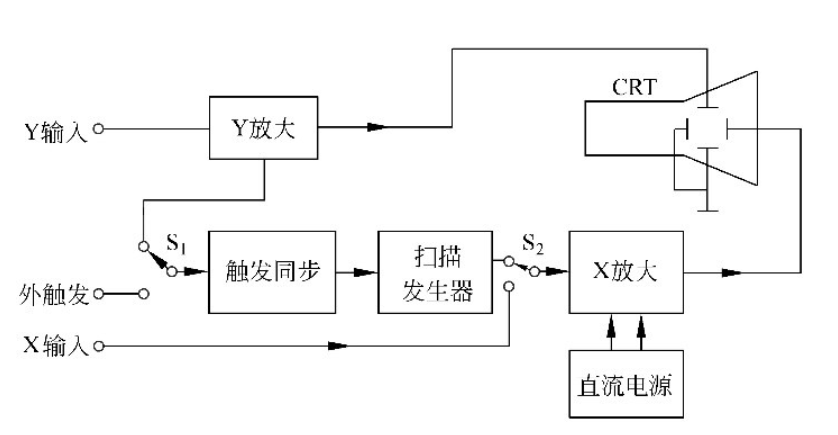
\includegraphics[scale=0.4]{示波器.png}
        \caption{示波器结构}
        \label{fig:label}
    \end{figure}


    \noindent (1) 示波管(CRT)的基本结构
    \begin{enumerate}
    \item 电子枪:由灯丝、阴极、控制栅极、第一阳极和第二阳极五部分组成。

    \item 偏转系统:由两对互相垂直的偏转板组成,一对竖直偏转板,一对水平偏转板。

    \item 荧光屏:屏上涂有荧光粉,电子打上去能够发出荧光,形成光斑。
    \end{enumerate}

    \begin{figure}[h]
        \centering
        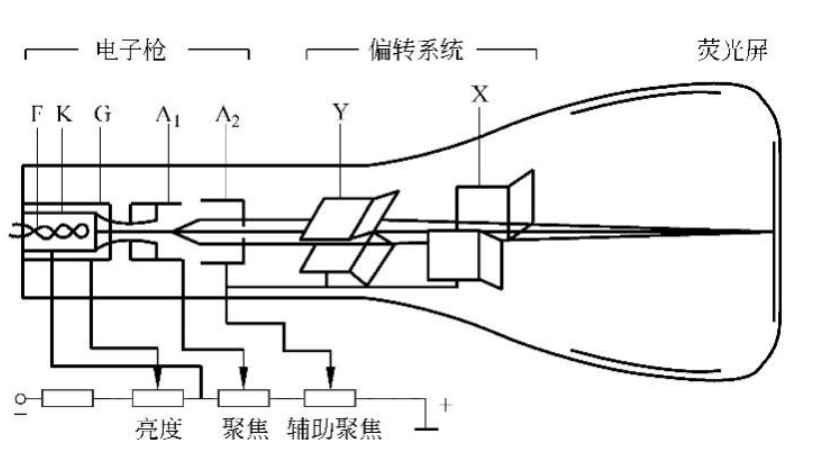
\includegraphics[scale=0.4]{示波管.png}
        \caption{示波管结构}
        \label{fig:label}
    \end{figure}

    \noindent (2) 示波器显示波形原理

    在竖直偏转板上加一交变的正弦电压,则电子束光斑将随电压的变化在竖直方向来回运动,
    同时在水平偏转板上加一扫描电压,使电子束光斑沿水平方向拉开,这样可以显示电压波形。

    \noindent (3) 同步触发

    如果正弦波和锯齿波电压的周期稍有不同,屏上显示的波形将会移动。
    可以通过调节“SCALE”(时间分度)调节旋钮,用来调节锯齿波电压的周期 $T_x$,
    使之与被测信号的周期$ T_y$ 成整数倍关系,从而在示波器屏幕上得到所需数目的完整波形。
    
    \noindent (4) 利萨如图形

    如果在示波器的 X 和 Y 输入端同时输入频率相同或成简单整数比的两个正弦波信号,则屏幕上的光斑
    将呈现特殊形状的轨迹,这种轨迹图称为利萨如图形。若已知其中一个信号的频率,
    数出图上的切点数 $n_x$ 和 $n_y$,便可算出另一待测信号的频率。

    \noindent (5) 数字示波器

    数字示波器主要工作原理为:被测信号输入→AD转换器转换为数字信号→采样记录存储→程序处理→波形复现到液晶屏幕。


    \subsection{声速测量}

    \noindent (1) 空气中的声速

    在理想气体中,声波的传播速度为
    $$
    v=\sqrt{\frac{\gamma R T}{\mu}}
    $$

    式中  $\gamma=c_{p} / c_{V}$  称为比热容比, 即气体定压比热容与定容比热容的比值,  $\mu$  为气体的摩尔质量, 
    $T $ 为绝对温 度,  $R=8.31441 \mathrm{~J} / \mathrm{mol} \cdot \mathrm{K}$  为普适气体常数。
    
    在正常情况下,干燥空气的平均摩尔质量$\mu_{a}=28.964 \times 10^{-3} \mathrm{~kg} / \mathrm{mol} $ 。
    在标准状态下,干燥空气中的声速 $v_0=331.5m/s$。在室温 $t^\circ C$下,干燥空气中的声速为:
    $$
    v=v_{0} \sqrt{1+\frac{t}{T_{0}}}
    $$  
    由于空气并不干燥,经过修正后得到在温度为 $t^\circ C$、相对湿度为 $r$ 的空气中,声速为:
    $$
    v=331.5 \sqrt{\left(1+\frac{t}{T_{0}}\right)\left(1+0.31 \frac{r p_{s}}{p}\right)}(\mathrm{m} / \mathrm{s})
    $$

    \noindent (2) 相位法测量声速
    
根据 $v=f\lambda$,测出声波的频率f和波长$\lambda$,即可测出声速。
在发射器的声波场中,找到某位置使接收器的电信号与发射器的电信号同相,
找到下一个同相点所移动的距离即为声波的波长。
可利用利萨如图形在两电信号同相时椭圆退化成右斜
直线来判断(斜直线情况判断相位差最为敏锐)。
    

\section{实验仪器}

\noindent TBS1102B-EDU数字示波器

\noindent AFG1062函数信号发生器

\noindent 自制多波形信号发生器

\noindent 数显式声速测量仪(包含声波发生器、超声波接收器、数显游标卡尺)

\noindent 干湿温度计

\noindent 已知参数的电容、电感、变压器

\noindent 导线若干、九孔面包板

\section{实验任务或步骤}

\subsection{示波器的原理和使用}
\noindent(1)用示波器分别测自制信号发生器输出的正弦波、三角波、方波、尖脉冲波数据。

\noindent(2)调整数信号发生器的1、2两路正弦信号频率比为1:1和2:1,改变初始相位,记录图像。

\noindent(3)将自制信号源和函数信号发生器正弦波信号输入到示波器输入端,观察利萨如图形。
\subsection{声速测量}
\noindent(1)连接电路,细调频率,使接收器输出信号最大。

\noindent(2)用相位法测波长。

\noindent(3)计算声速理论值,与实验测得的声速值比较。
\subsection{电路设计与测量}

\noindent(1)从电容器的充放电波形到三角波

\noindent(2)尖脉冲产生原理探究

\noindent(3)相位变化的观测

\noindent(4)共振电路测电感、电容

\section{数据处理}
\subsection{示波器的原理和使用}

\subsubsection{波形观测}
\begin{center}
    \begin{tabular}{|c|c|c|c|}
     
        \hline  &峰峰值$U_{p-p}/V$&周期$T/ \mu s$&频率$f/kHz$\\
        \hline  正弦波&5.68&709.0&1.410\\
        \hline  三角波&7.76&709.0&1.406\\
        \hline  方波&8.88&708.8&1.411\\
        \hline  尖脉冲波&16.8&710.0&1.408\\
        \hline
    
    \end{tabular}
\end{center}

绘制屏幕波形如图3:
 
\begin{figure}[h]
    \centering
    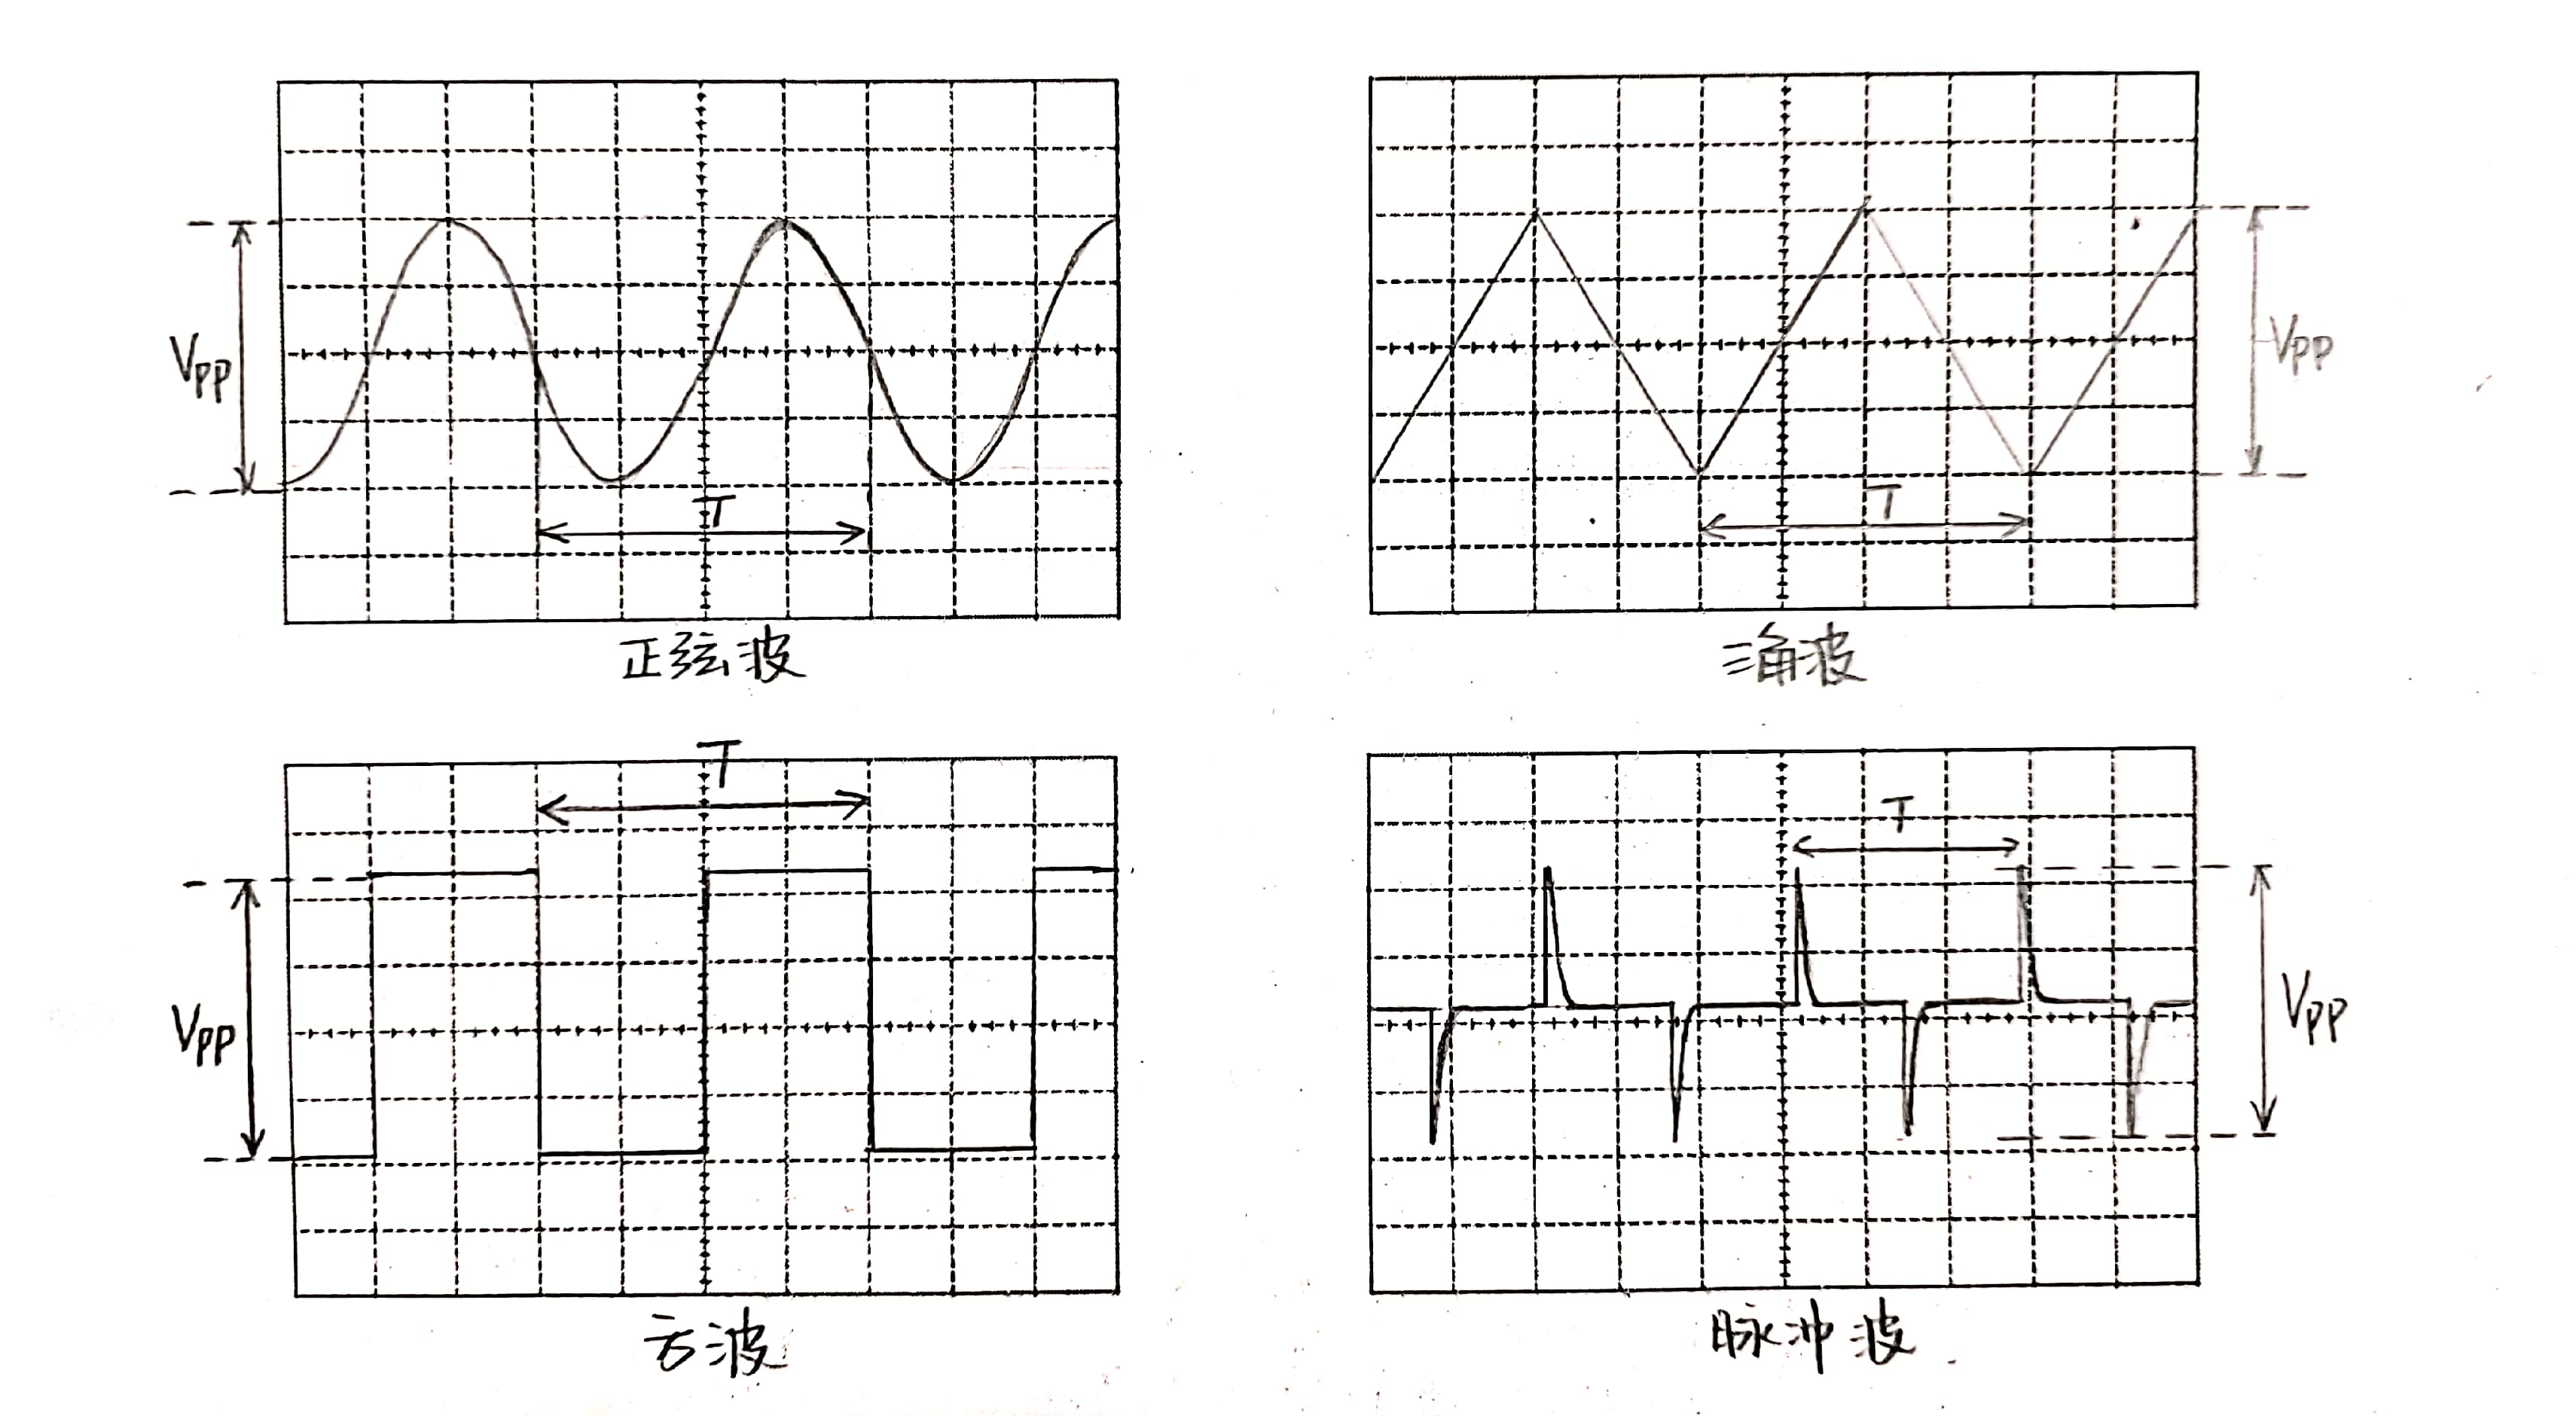
\includegraphics[scale=0.15]{手绘波形.jpg}
    \caption{手绘波形}
    \label{fig:label}
\end{figure}


其中正弦波的幅度有效值为幅值的$\frac{ \sqrt{2}}{2}$倍,即为$\frac{5.68}{\sqrt{2}}=2.01V$。

所以有:

正弦波的幅度有效值:2.01V
 
方波的幅度值:8.88V

三角波的周期:708.8$\mu s$

尖脉冲的频率:1.408 kHz




\subsubsection{观察利萨如图形}

\noindent (1)观察函数信号发生器的两路正弦信号

$f_x=f_y=5kHz$,$f_x:f_y=1:1$时:

\begin{figure}[h]
    \centering
    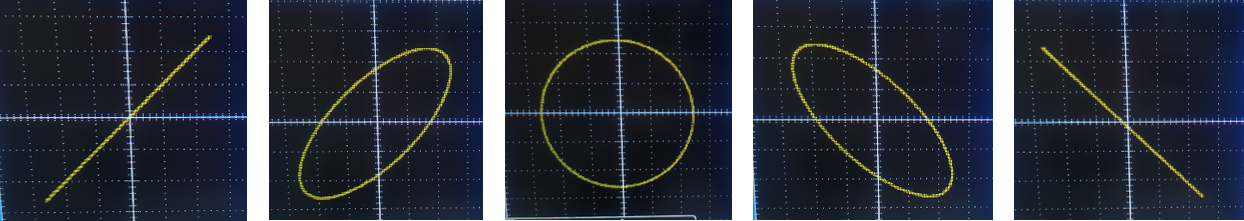
\includegraphics[scale=0.8]{1:1的图像.png}
    \caption{从左至右相位差依次为:$0,\frac{\pi}{4},\frac{\pi}{2},\frac{3\pi}{4},\pi$}
    \label{fig:label}
\end{figure}

$f_x=5kHz,f_y=2.5kHz$,$f_x:f_y=2:1$时:
\begin{figure}[h]
    \centering
    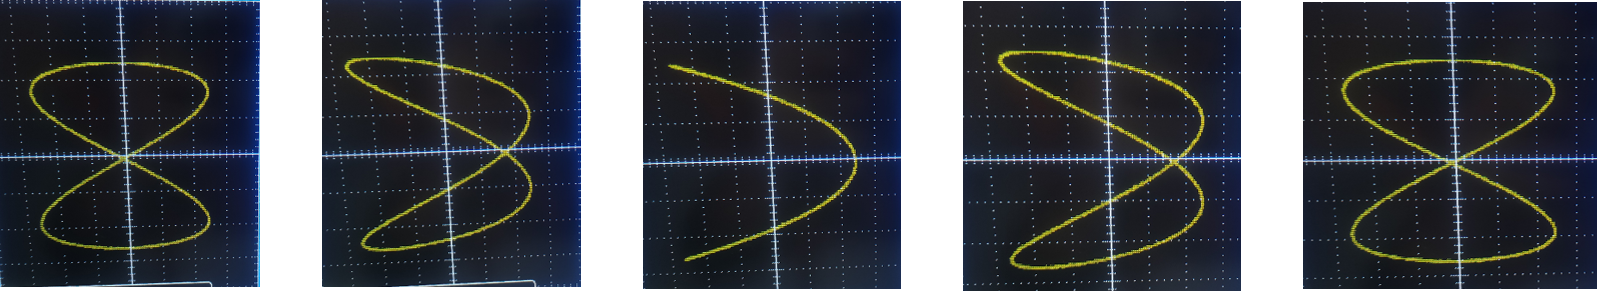
\includegraphics[scale=0.6]{2:1.png}
    \caption{$\Phi_y =0$,从左至右$\Phi_x$依次为:$0,\frac{\pi}{4},\frac{\pi}{2},\frac{3\pi}{4},\pi$.}
    \label{fig:label}
\end{figure}

\begin{figure}[h]
    \centering
    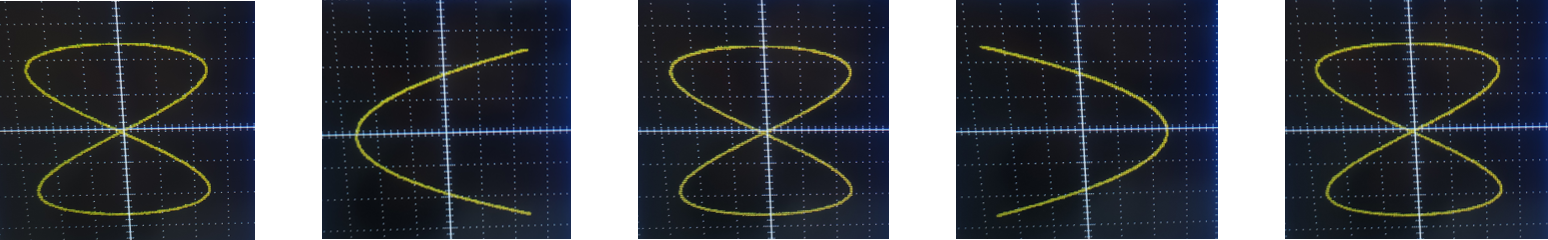
\includegraphics[scale=0.62]{2:1第二种.png}
    \caption{$\Phi_x =0$,从左至右$\Phi_y$依次为:$0,\frac{\pi}{4},\frac{\pi}{2},\frac{3\pi}{4},\pi$.}
    \label{fig:label}
\end{figure}

我们发现,x相位超前于y和y相位超前于x在$f_x:f_y=2:1$时对利萨如图形的影响有所不同,
这是因为他们周期不同带来的差异。
\\
\\

\noindent (2)观察自制信号发生器的正弦信号

调出频率比 $f_x : f_y = 1 : 1$ 的利萨如图形并使图形尽量稳定不变。

此时读函数信号发生器得频率为 $f_x = 1.935kHz$,因此测得自制正弦波的频率为 $f_y = f_x = 1.935kHz$。

所以:自制正弦波形频率为 $1.935 kHz$

\subsection{声速测量}

\noindent (1)测量条件
\begin{center}
    \begin{tabular}{|c|c|c|}
        \hline  时间&温度$/^\circ C$&相对湿度/\%\\
        \hline  实验前&21.1&48.1\\
        \hline  实验后&21.1&47.9\\
        \hline
    \end{tabular}
\end{center}

由此可算得:

$$
\bar{t}=21.1^{\circ} \mathrm{C}, \quad \bar{r}=48.0 \%
$$

根据线性内插法计算得:

$$
p_{s}=[0.0249+(0.0264-0.0249) \times(21.1-21)] \times 10^{5}=0.02505 \times 10^{5} \mathrm{~Pa}
$$

故声速的理论值:

\begin{align}
    v&=331.5 \sqrt{\left(1+\frac{t}{T_{0}}\right)\left(1+0.31 \frac{r p_{s}}{p}\right)}(\mathrm{m} / \mathrm{s}) \nonumber \\
    &=331.5\times \sqrt{\left(1+\frac{21.1}{273.15}\right)\left(1+0.31\times \frac{0.48 \times 0.02505 \times 10^{5}}{1.013 \times 10^{5}}\right)}(\mathrm{m} / \mathrm{s}) \nonumber\\
    &= 344.698\mathrm{~m} / \mathrm{s} \nonumber
\end{align}




\noindent (2)细调频率,使得接收器输出信号最大
$$
f=40.800kHz
$$

\noindent (3)用相位法测量波长
 
\noindent 测量数据如下:
\begin{center}
    \begin{tabular}{|c|c|c|c|}
        \hline  序号&$x_i/mm $&$x_{i+10}/mm $&$L_i=x_{i+10}-x_i$\\
        \hline  1&15.37&101.32&85.95\\
        \hline  2&24.01&108.96&84.95\\
        \hline  3&32.70&116.95&84.25\\
        \hline  4&41.35&124.84&83.49\\
        \hline  5&49.75&133.35&83.60\\
        \hline  6&58.32&141.76&83.44\\
        \hline  7&66.77&150.46&83.69\\
        \hline  8&75.23&159.25&84.02\\
        \hline  9&83.90&168.09&84.19\\
        \hline  10&92.62&176.92&84.30\\
        
        \hline
    \end{tabular}
\end{center}

\textbf{利用逐差法求解,有:}
$$
10 \bar{\lambda}=\frac{\sum\left(x_{i+10}-x_{i}\right)}{10}=84.188 \mathrm{~mm}
$$
$$
\bar{\lambda}=8.4188mm
$$
$$
v=f\lambda=343.487m/s
$$
根据公式:
$$
\Delta_{10 \lambda}=\sqrt{\left(\frac{t}{\sqrt{n}} S_{10 \lambda}\right)^{2}+(\sqrt{2} \Delta)^{2}}
$$
计算$10\lambda$的标准差为:
$$
S_{10 \lambda}=\sqrt{\frac{\sum\left(10 \lambda_{i}-10 \bar{\lambda}\right)^{2}}{n-1}}=0.772468 \mathrm{~mm}
$$
查表知当置信概率 $ P=0.95$  时
$$
t_{p}(v)=2.26
$$
本实验数显游标卡尺不确定度  $\Delta  = 0.03 m m$  由于  $n  = 10$ , 将上述数据代入公式得
    
\begin{align}
    &\Delta_{10 \lambda}  = 0.553691 \mathrm{~mm}\nonumber \\
    &\Delta_{\lambda}  =\frac{1}{10} \Delta_{10 \lambda}= 0.0553691\mathrm{~mm}\nonumber
\end{align}

\noindent 频率的不确定度为10Hz,代入公式计算如下:
\begin{align}
    \frac{\Delta_{v}}{v} & = \sqrt{\left(\frac{\partial \ln v}{\partial f}\right)^{2} \cdot\left(\Delta_{f}\right)^{2}+\left(\frac{\partial \ln v}{\partial \lambda}\right)^{2} \cdot\left(\Delta_{\lambda}\right)^{2}} \nonumber\\
     & = \sqrt{\left(\frac{\Delta_{f}}{f}\right)^{2}+\left(\frac{\Delta \lambda}{\lambda}\right)^{2}}\nonumber\\
     & =0.00658141\nonumber
\end{align}

$$
\Delta_v=v\cdot\frac{\Delta_{v}}{v} =0.00658141\times343.487=2.26062m/s
$$

\noindent 综上所述:
\begin{align}
    &\lambda=\bar{\lambda} \pm \Delta \lambda=8.418\pm 0.055 mm\nonumber\\
    &v=343.5\pm 2.3 m/s\nonumber
\end{align}

\noindent \textbf{利用最小二乘法求解,有:}
\begin{figure}[h]
    \centering
    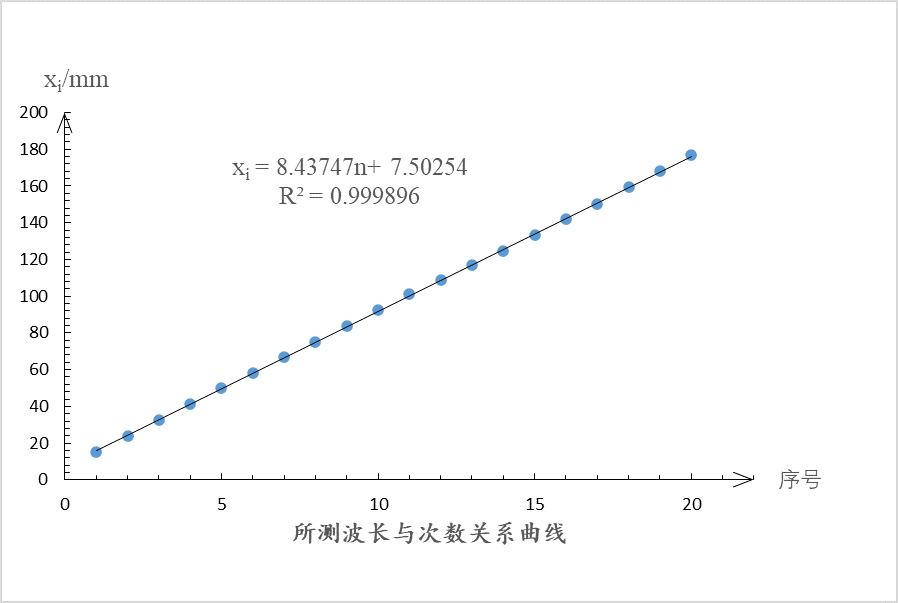
\includegraphics[scale=0.75]{波长拟合曲线.png}
    \caption{所测波长与次数的关系曲线}
    \label{fig:label}
\end{figure}

利用最小二乘法计算,得到直线斜率$k=8.43747$,即$\lambda=8.43747mm$。

相关系数$R^2=0.999896$,表示线性相关性较强。

则有:$v=f\lambda=344.2m/s $

\subsection{电路设计与测量}
\subsubsection{从电容器的充放电波形到三角波}

初始条件:$f=1kHz,R=10k\Omega,C=10.435nF$

f=1kHz,增大R,观察波形变化(水平和垂直定标均为1V/DIV):
\begin{figure}[htbp]
    \centering
    \subfigure[$R=10k\Omega$]{
        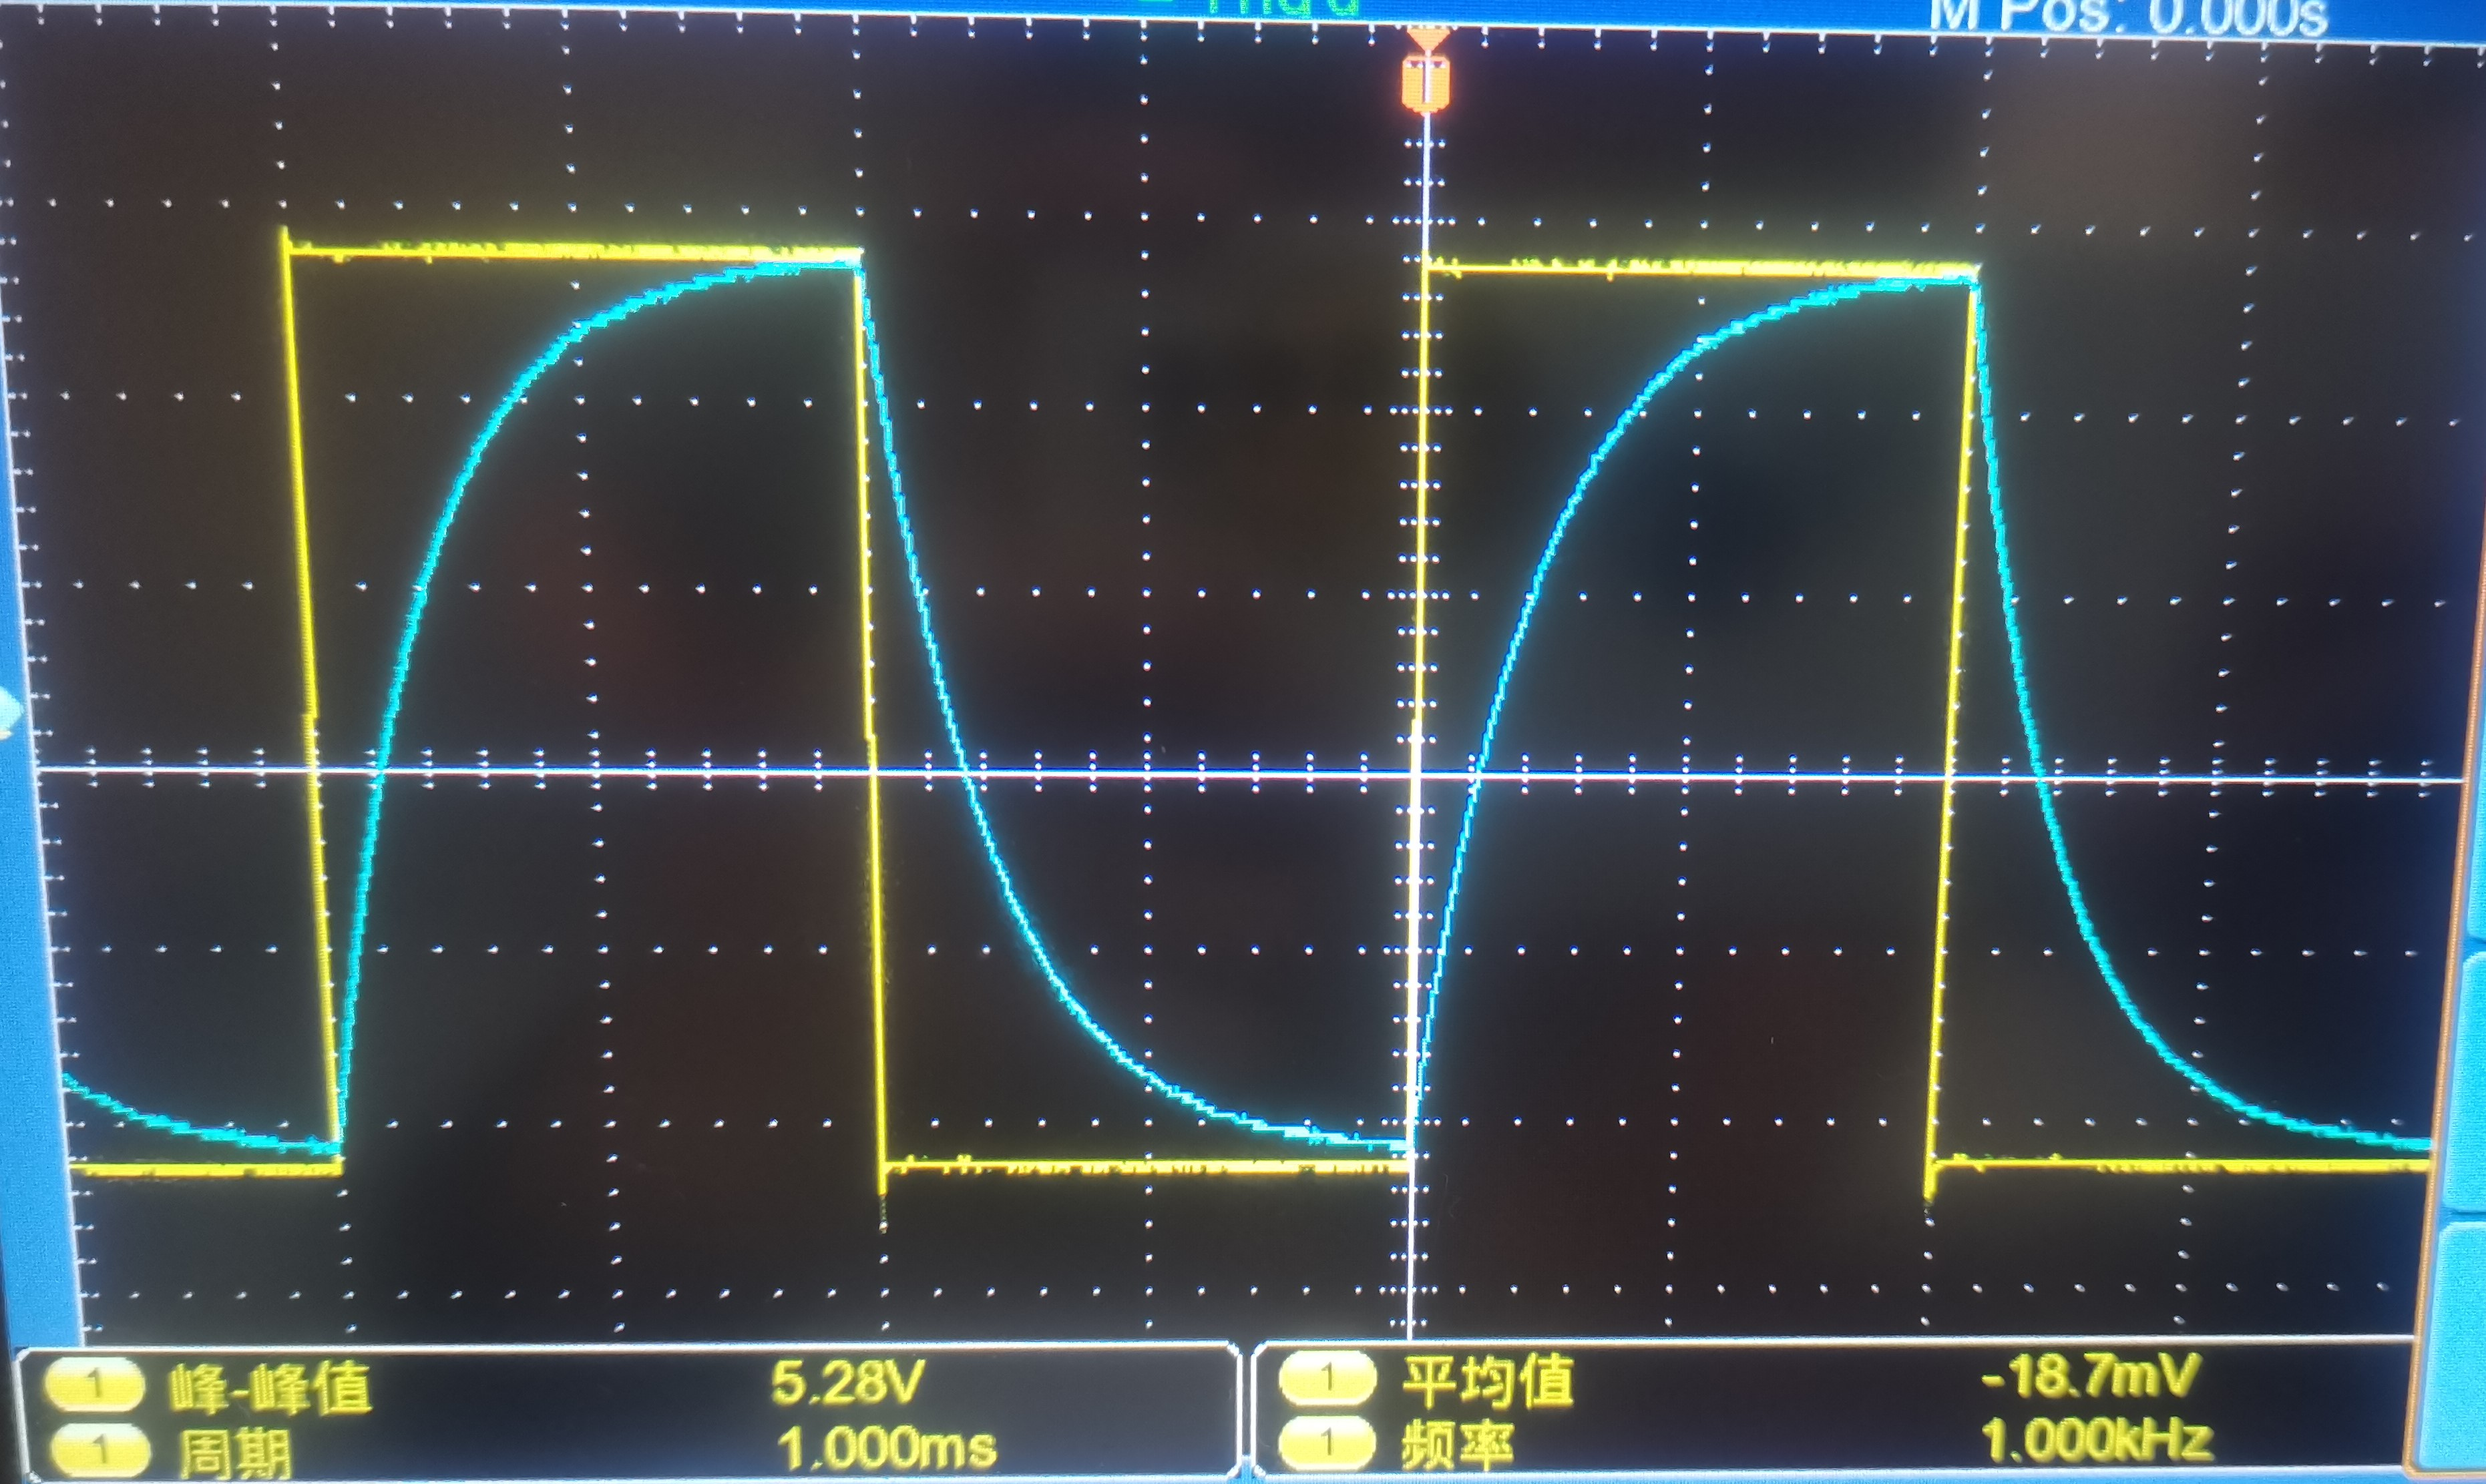
\includegraphics[width=2in]{10k.jpg}
    }
    \subfigure[$R=20k\Omega$]{
	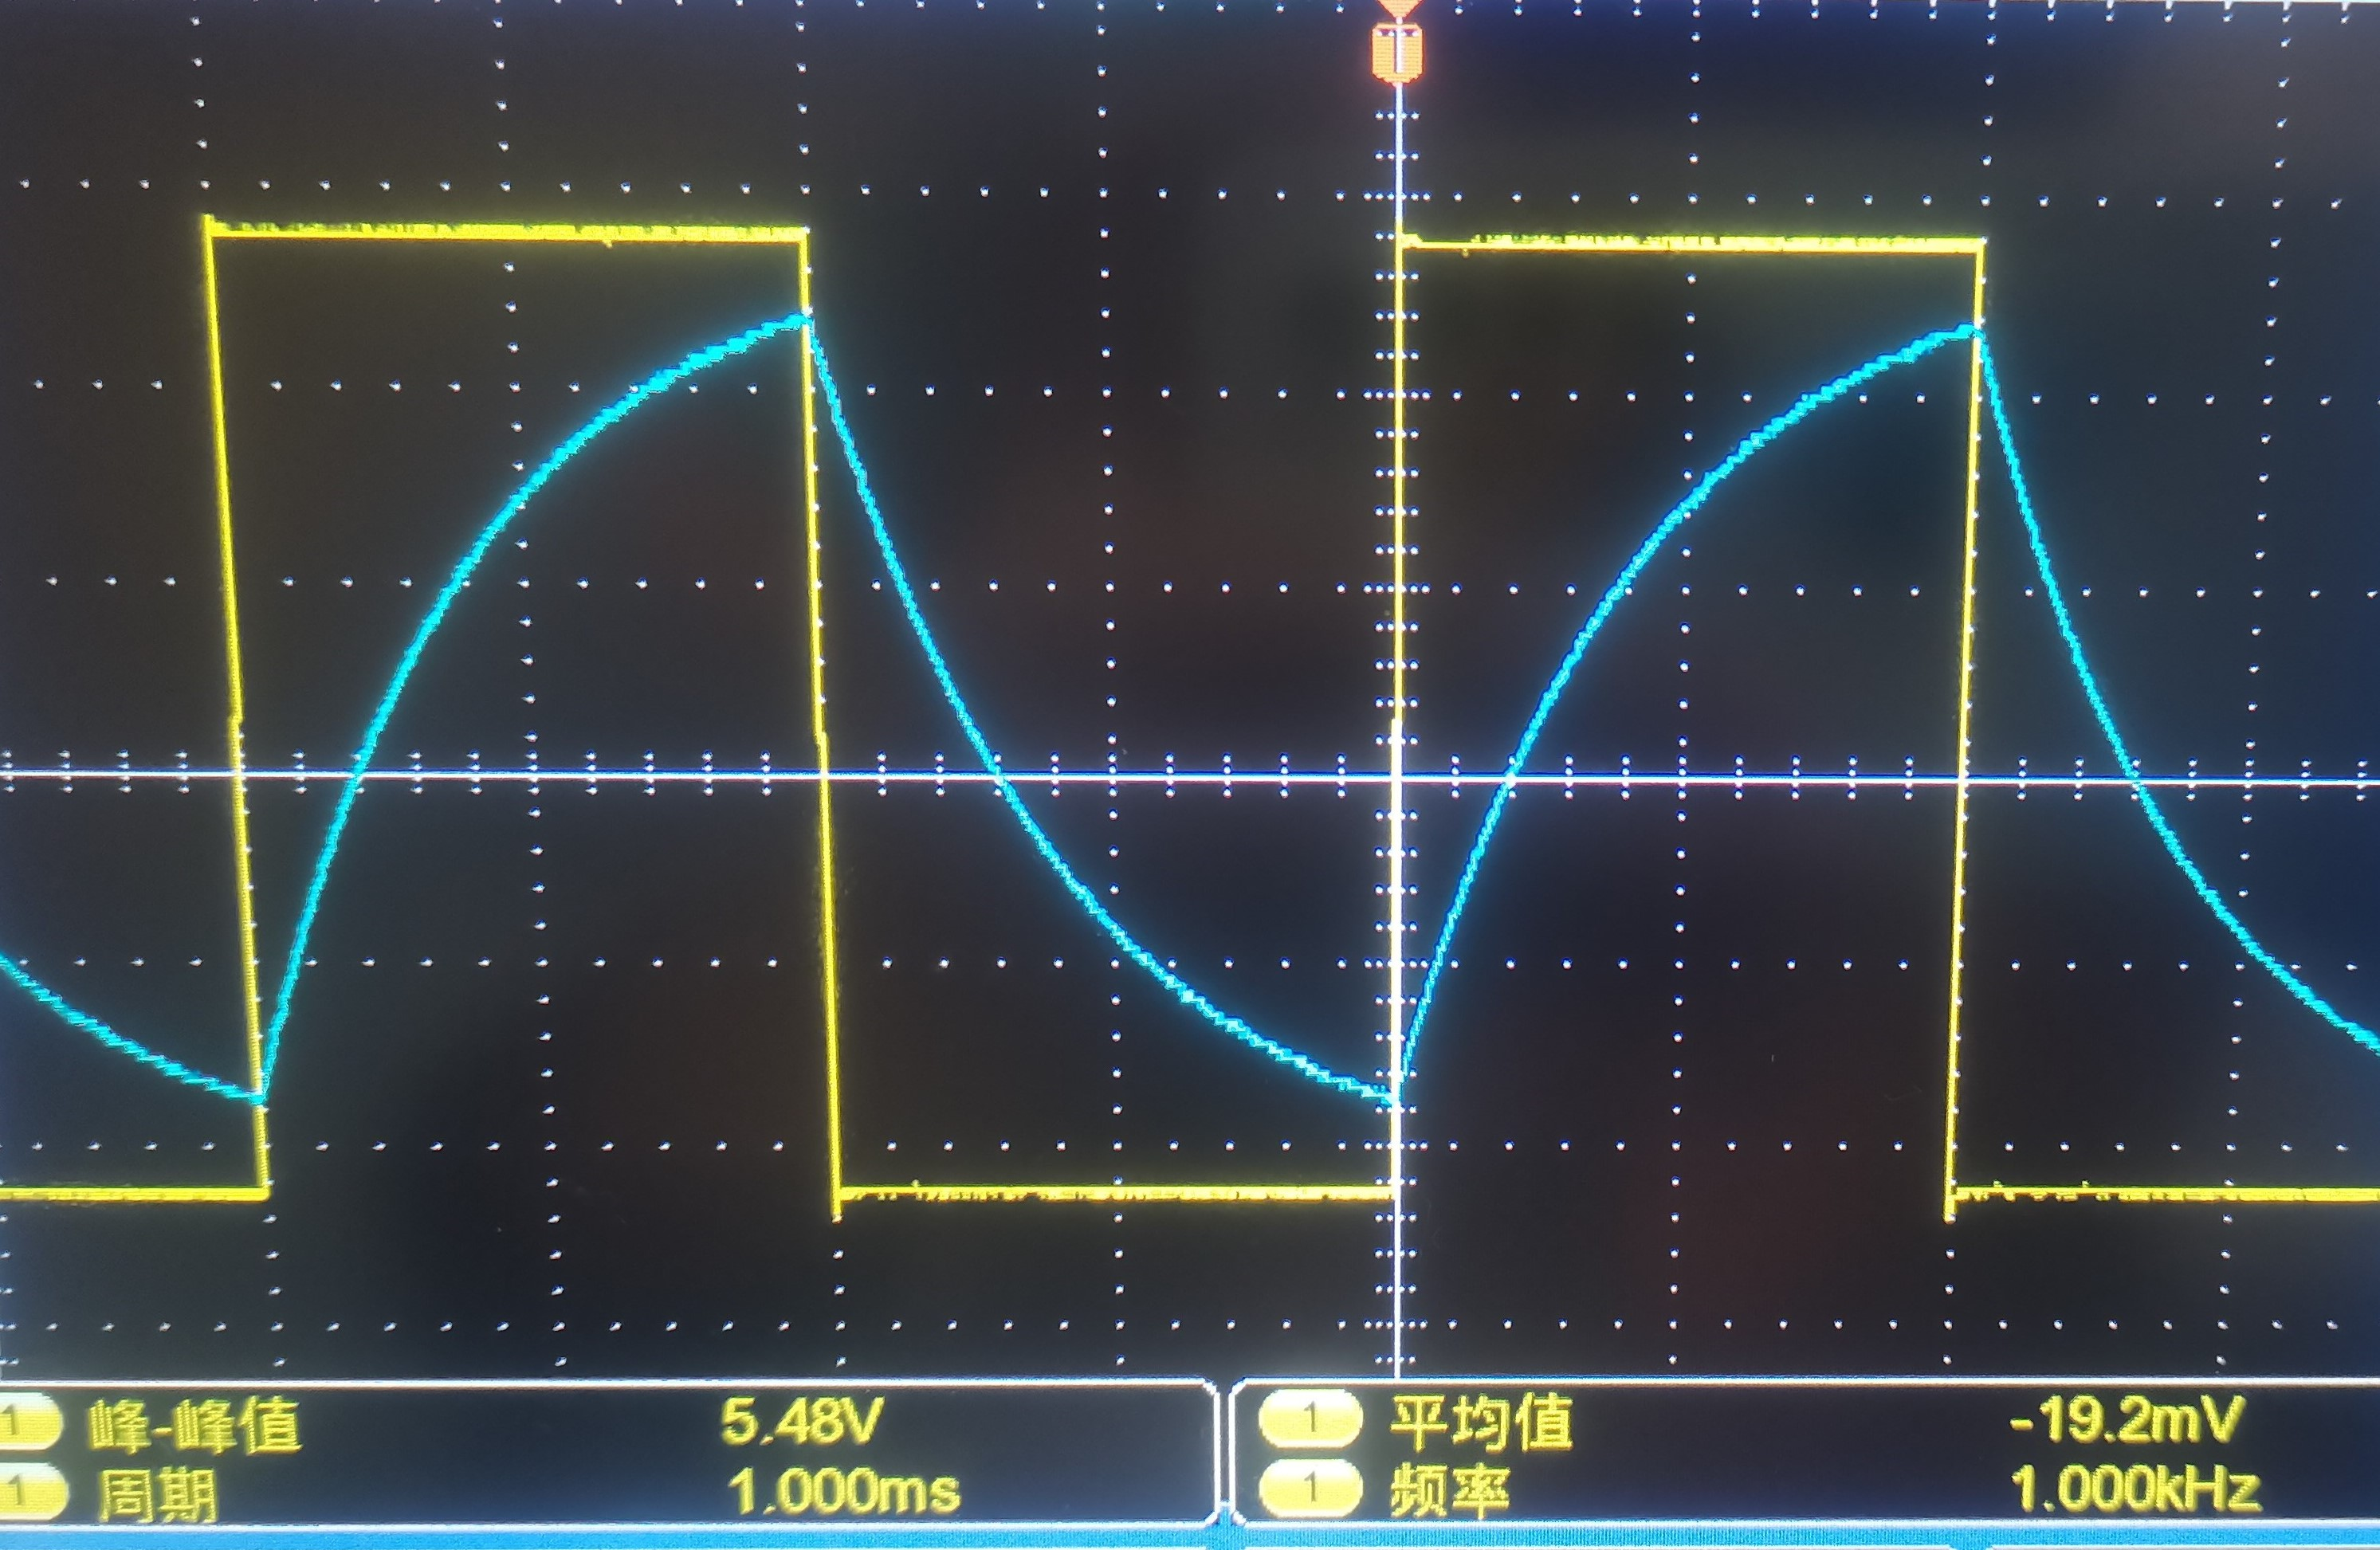
\includegraphics[width=1.9in]{20k.jpg}
    }
    \quad   
    \subfigure[$R=50k\Omega$]{
    	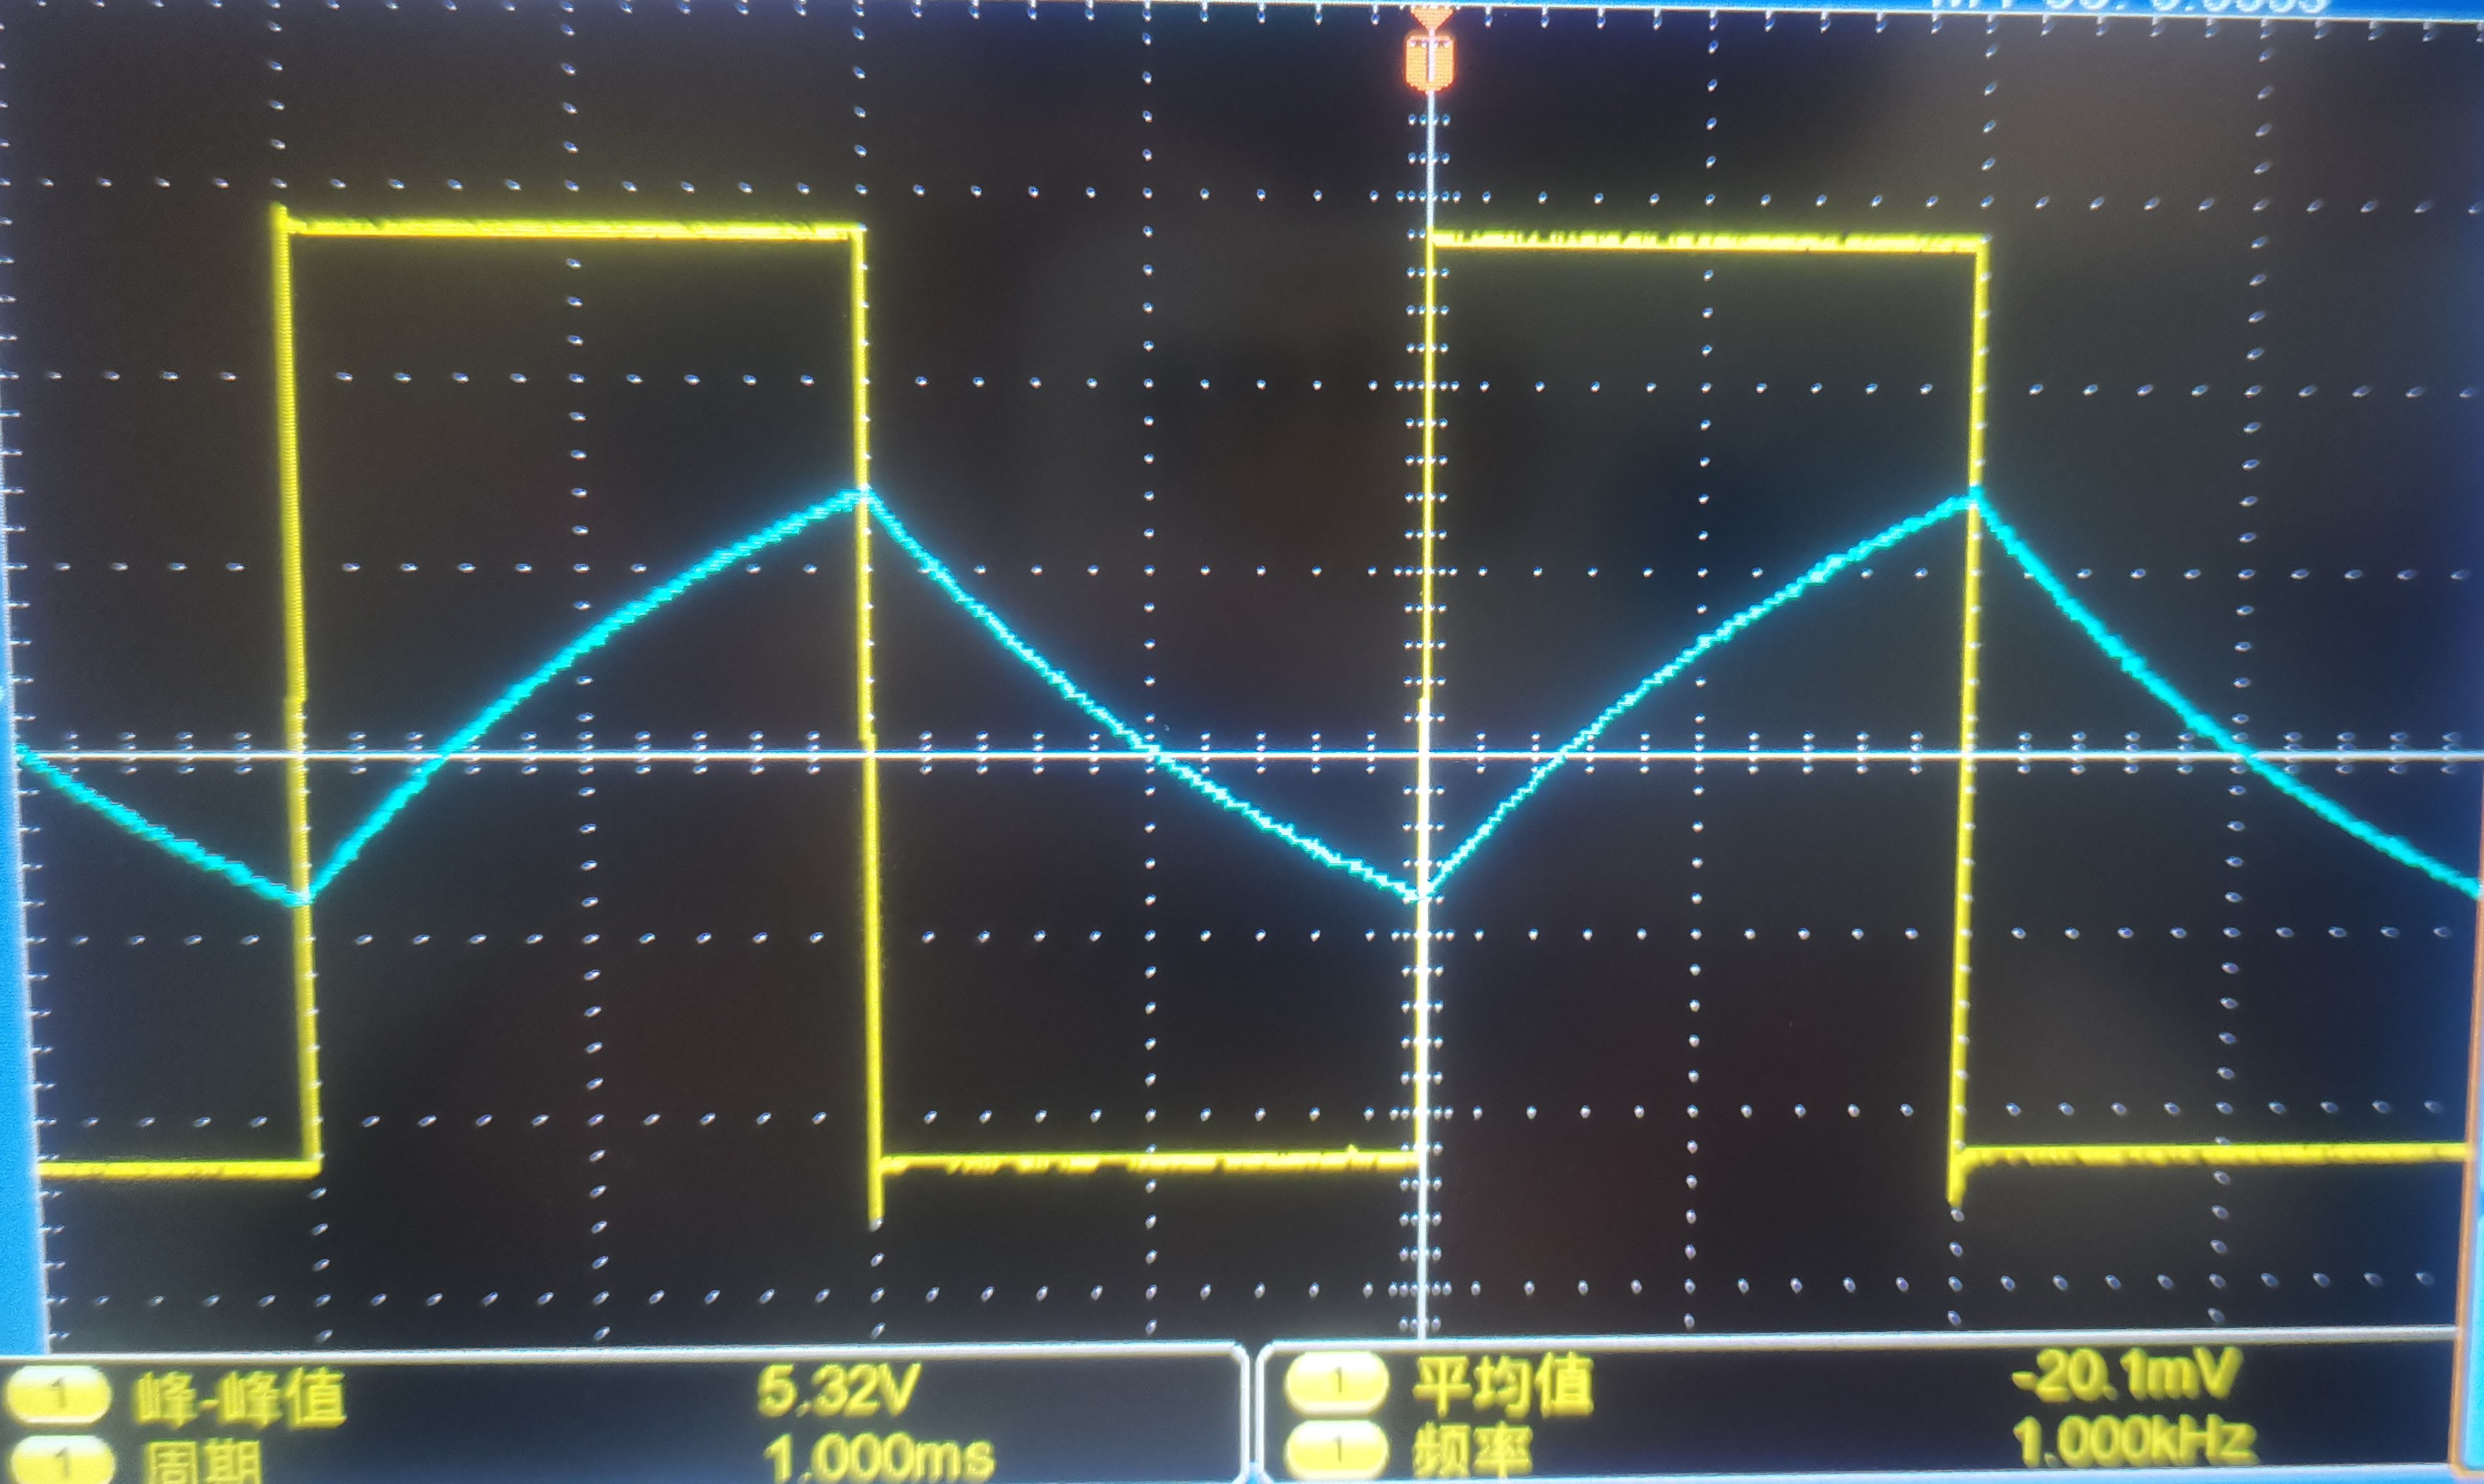
\includegraphics[width=1.9in]{50k.jpg}
    }
    \subfigure[$R=90k\Omega$]{
	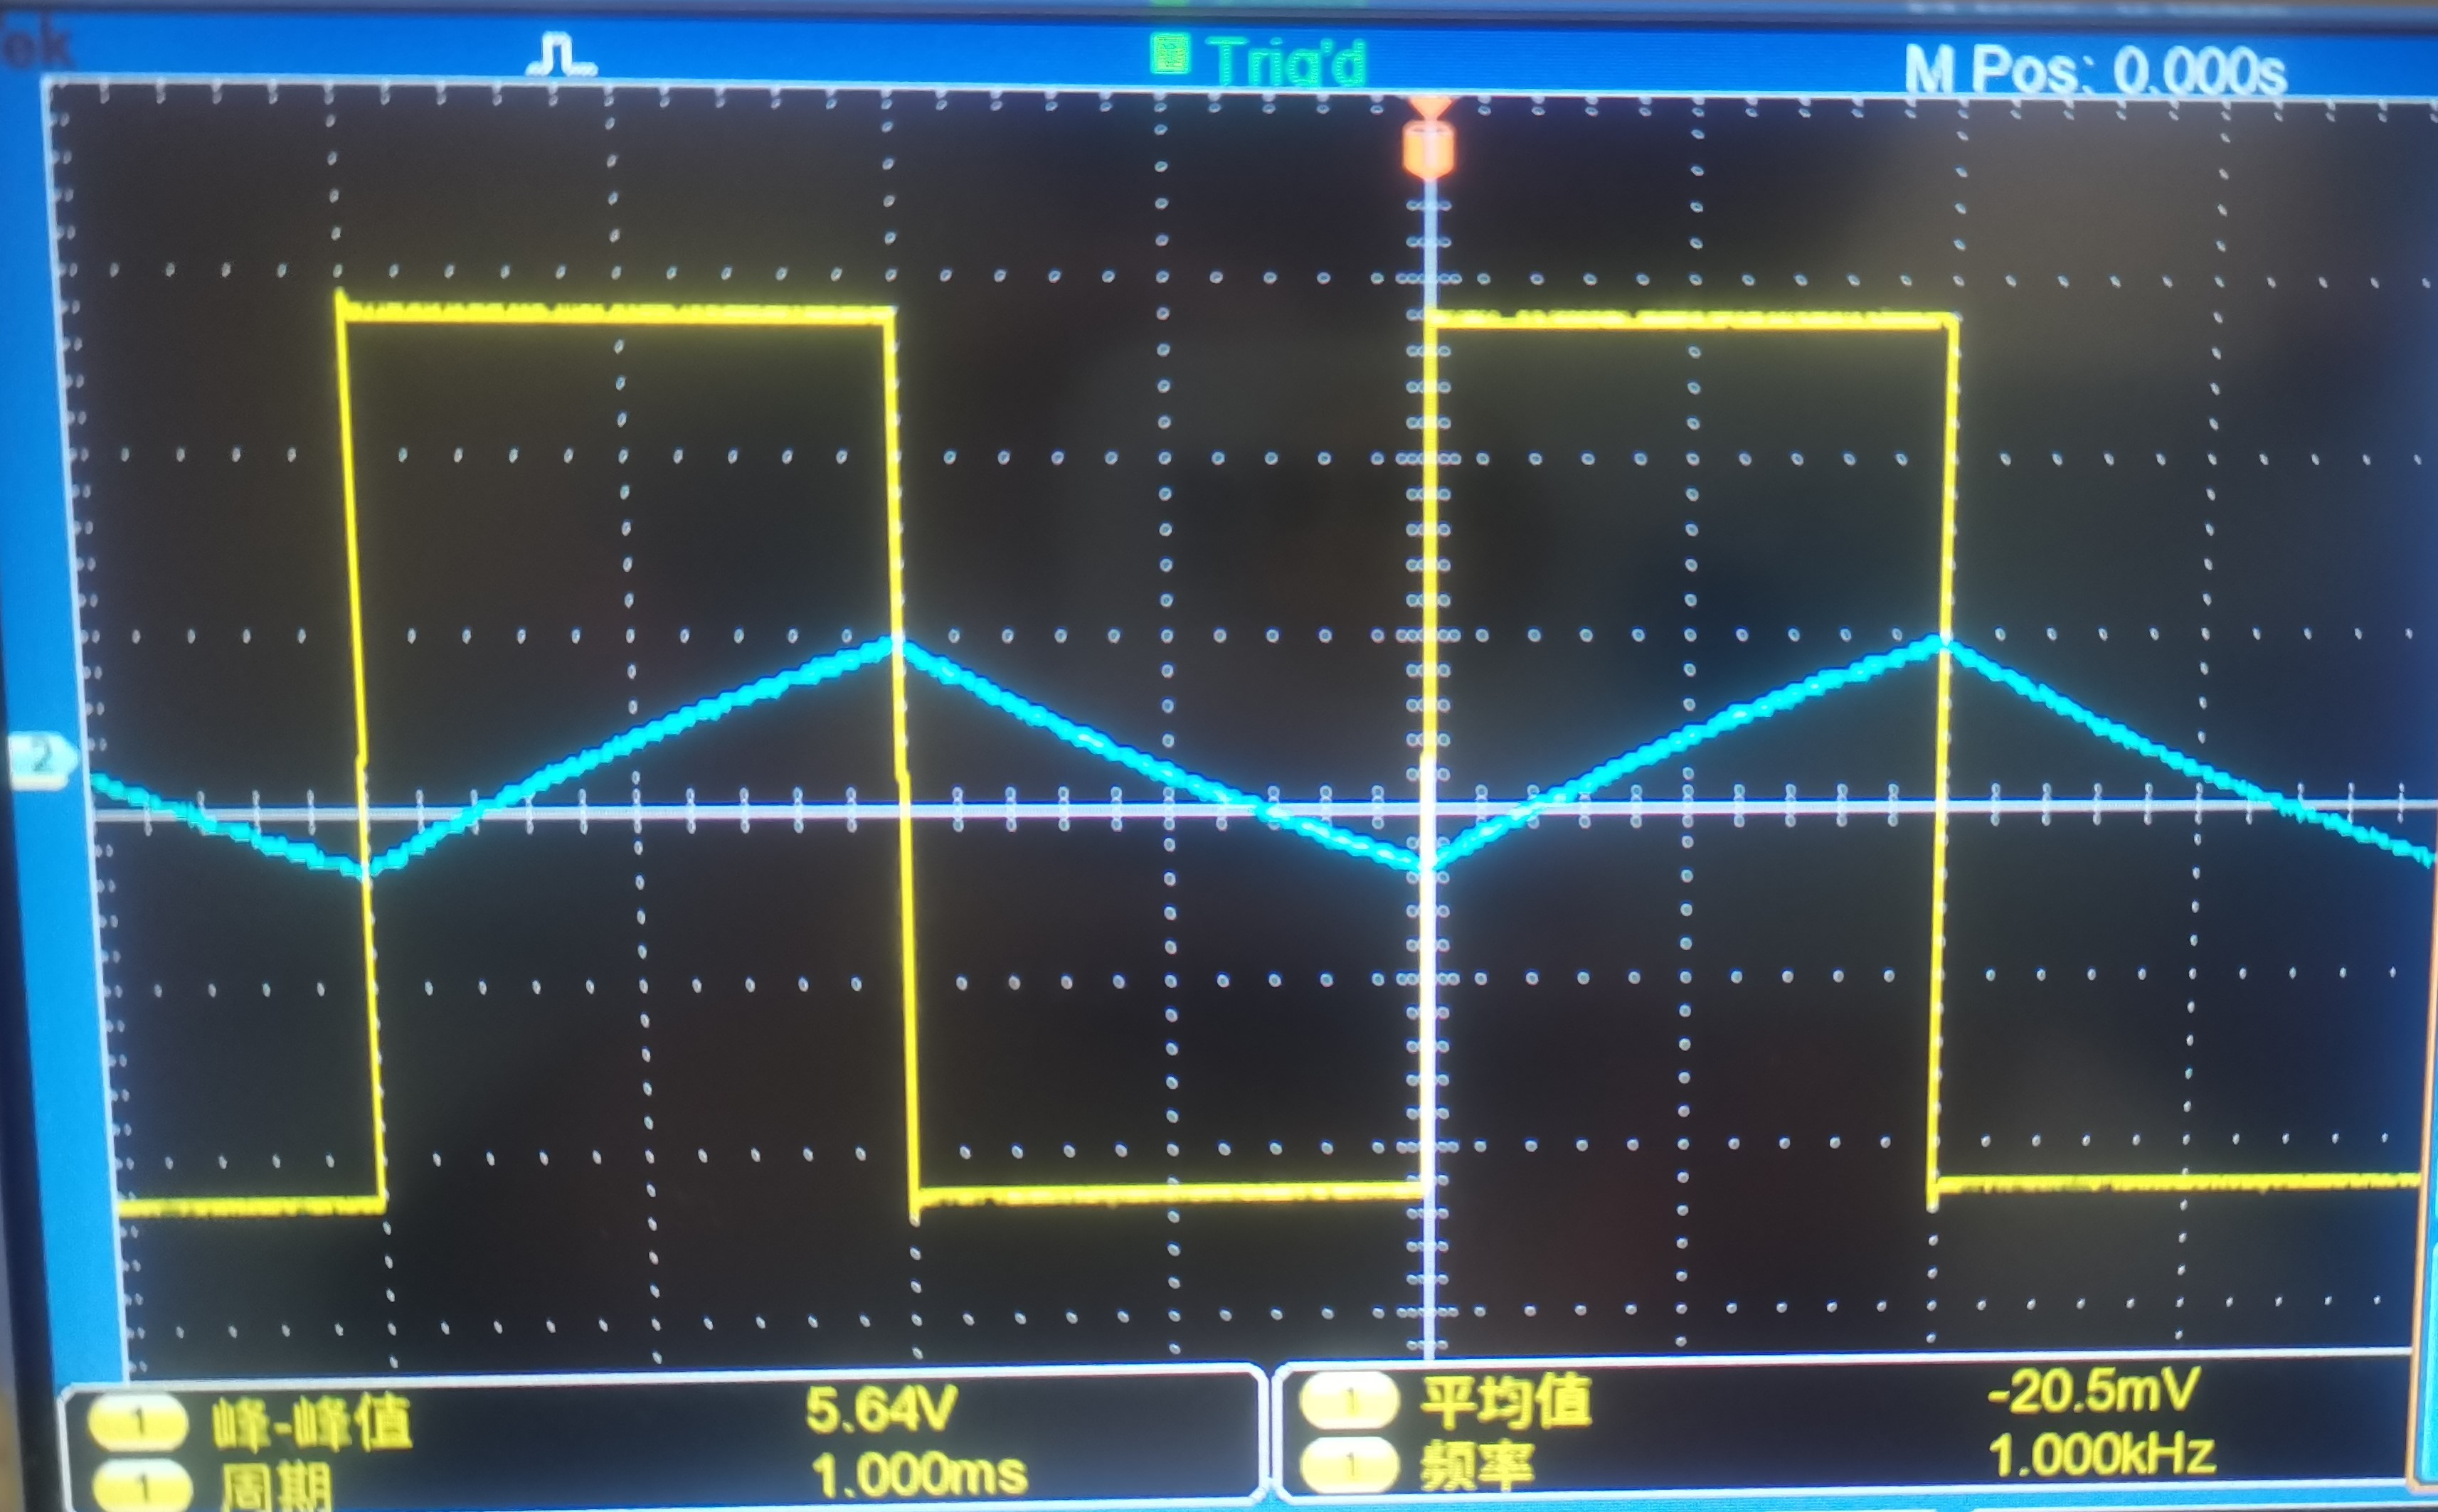
\includegraphics[width=1.9in]{90k.jpg}
    }
    \caption{$f=1kHz$ , 逐渐增大R}
    \label{fig.1}
\end{figure}

R=10k$\Omega$,增大f,观察波形变化(垂直定标为1V/DIV,水平定标根据频率有所调整):

\begin{figure}[htbp]
    \centering
    \subfigure[$f=1kHz$]{
        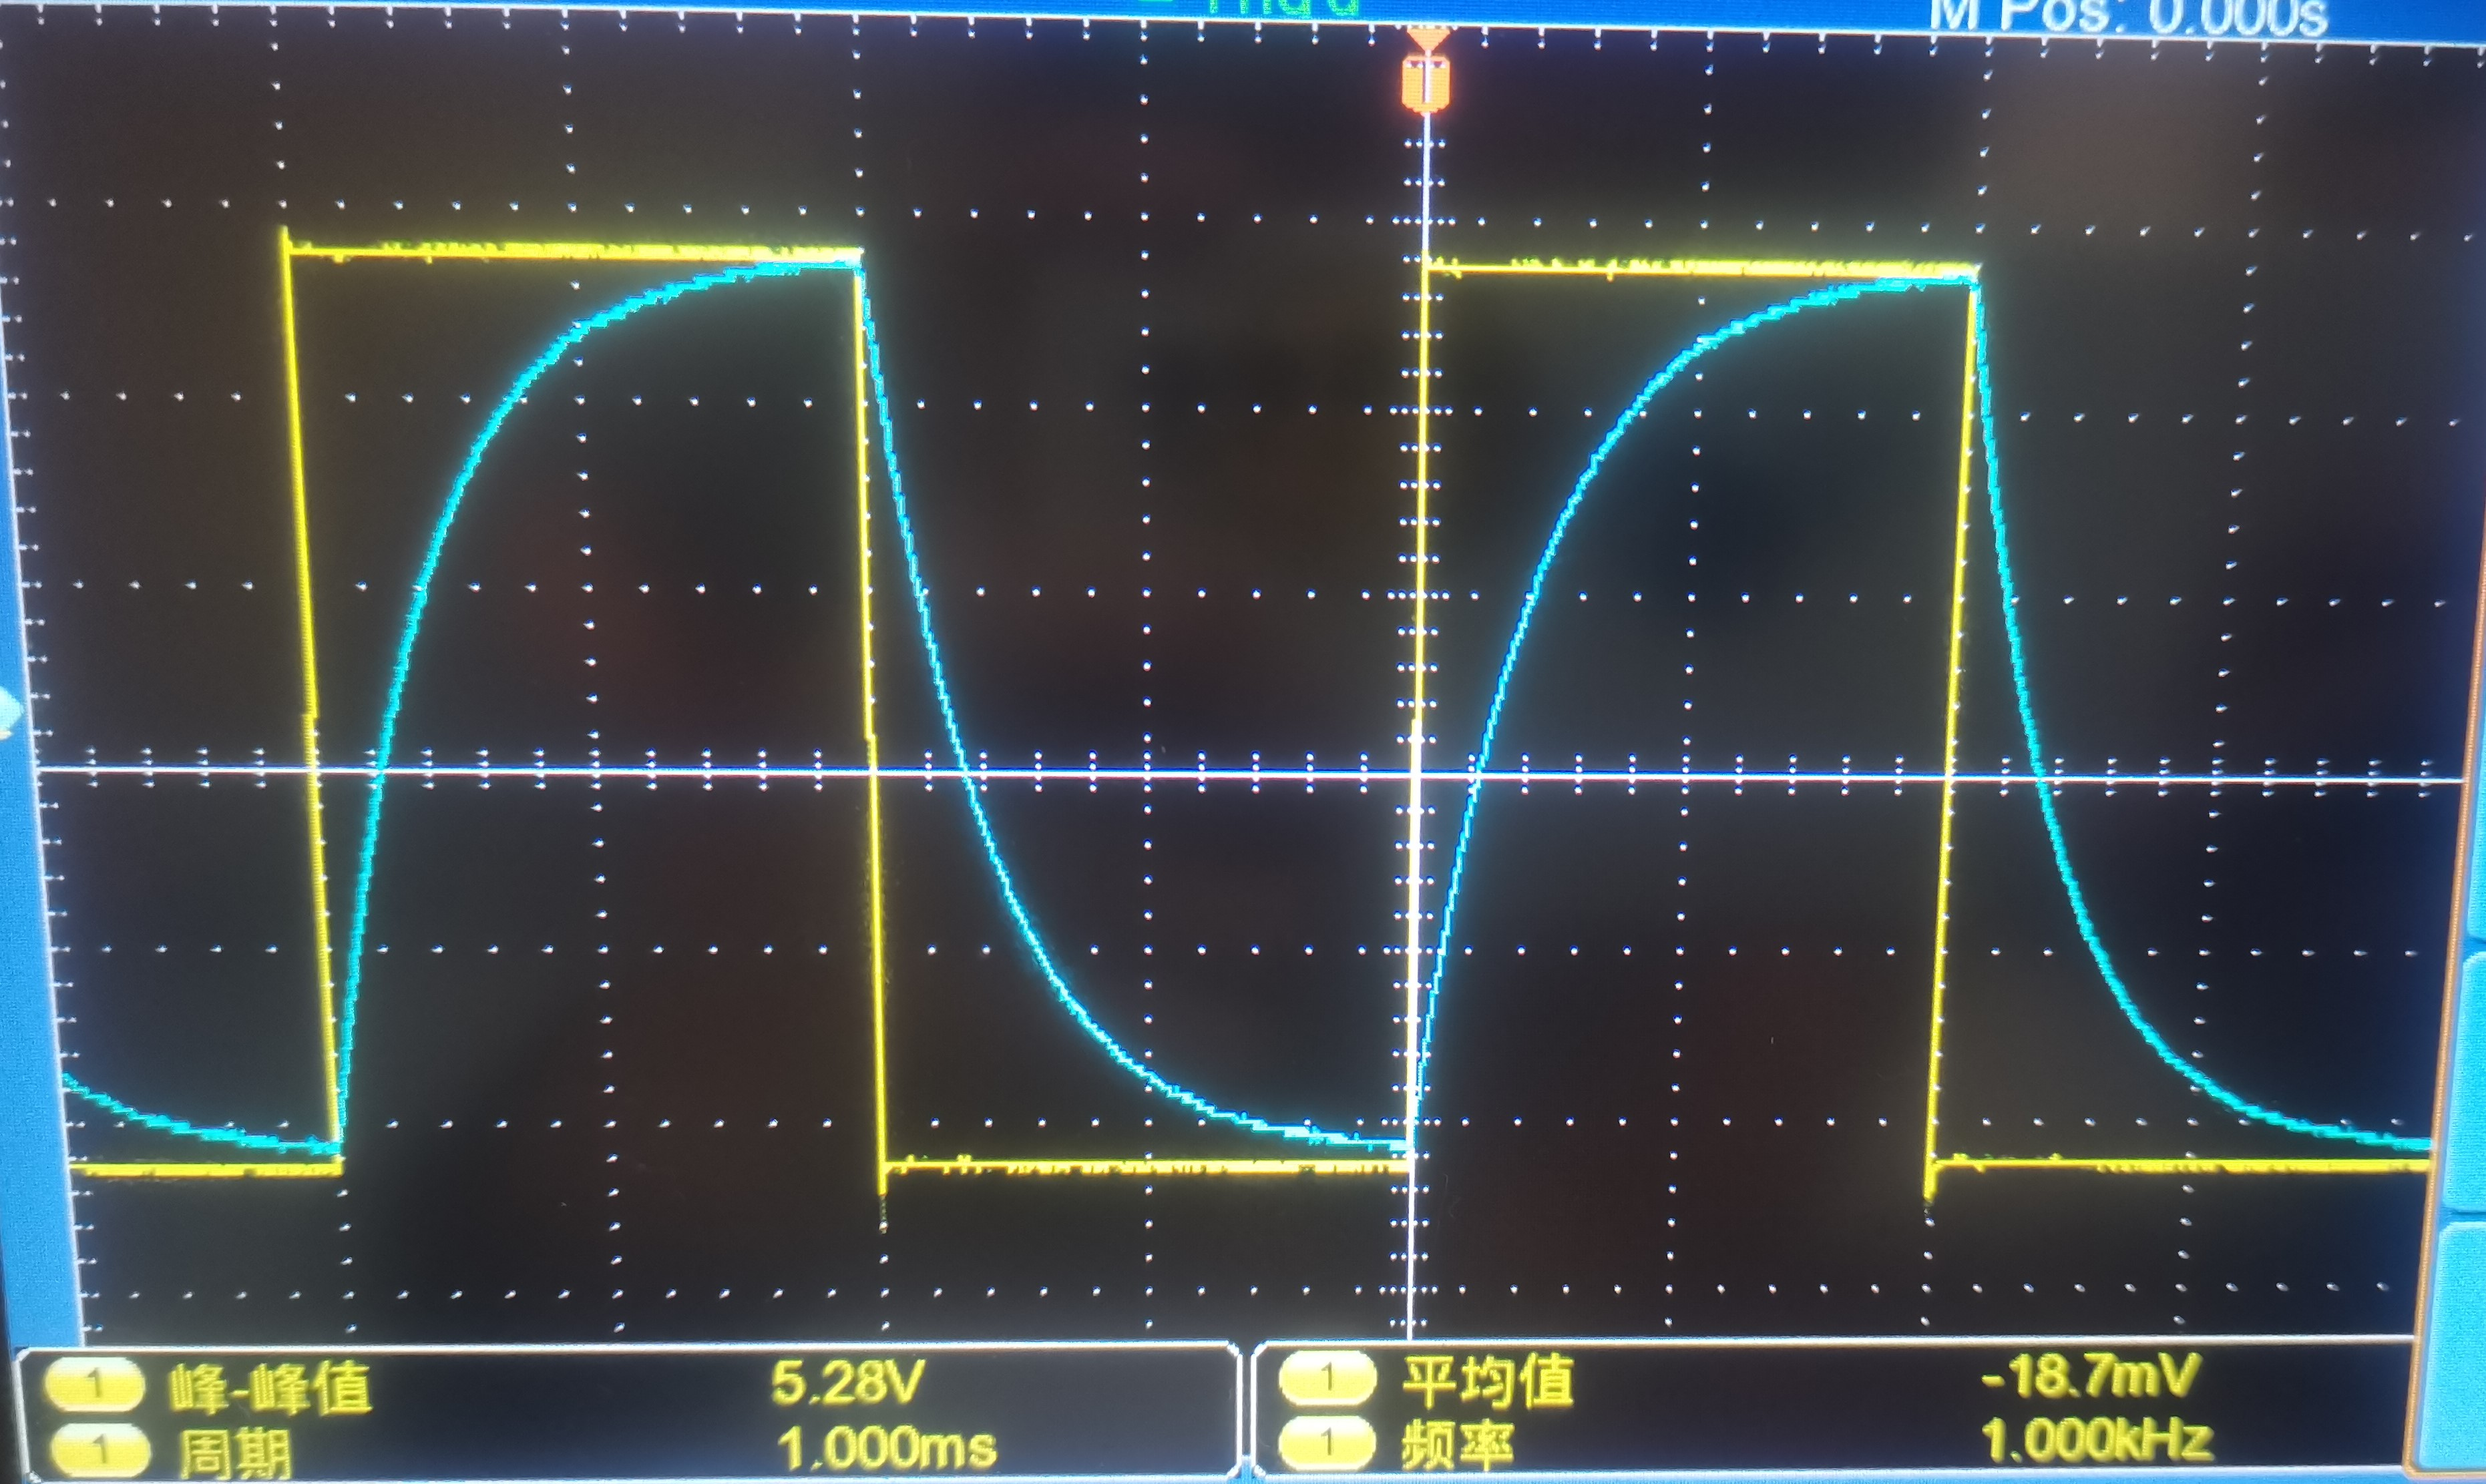
\includegraphics[width=2in]{10k.jpg}
    }
    \subfigure[$f=2kHz$]{
	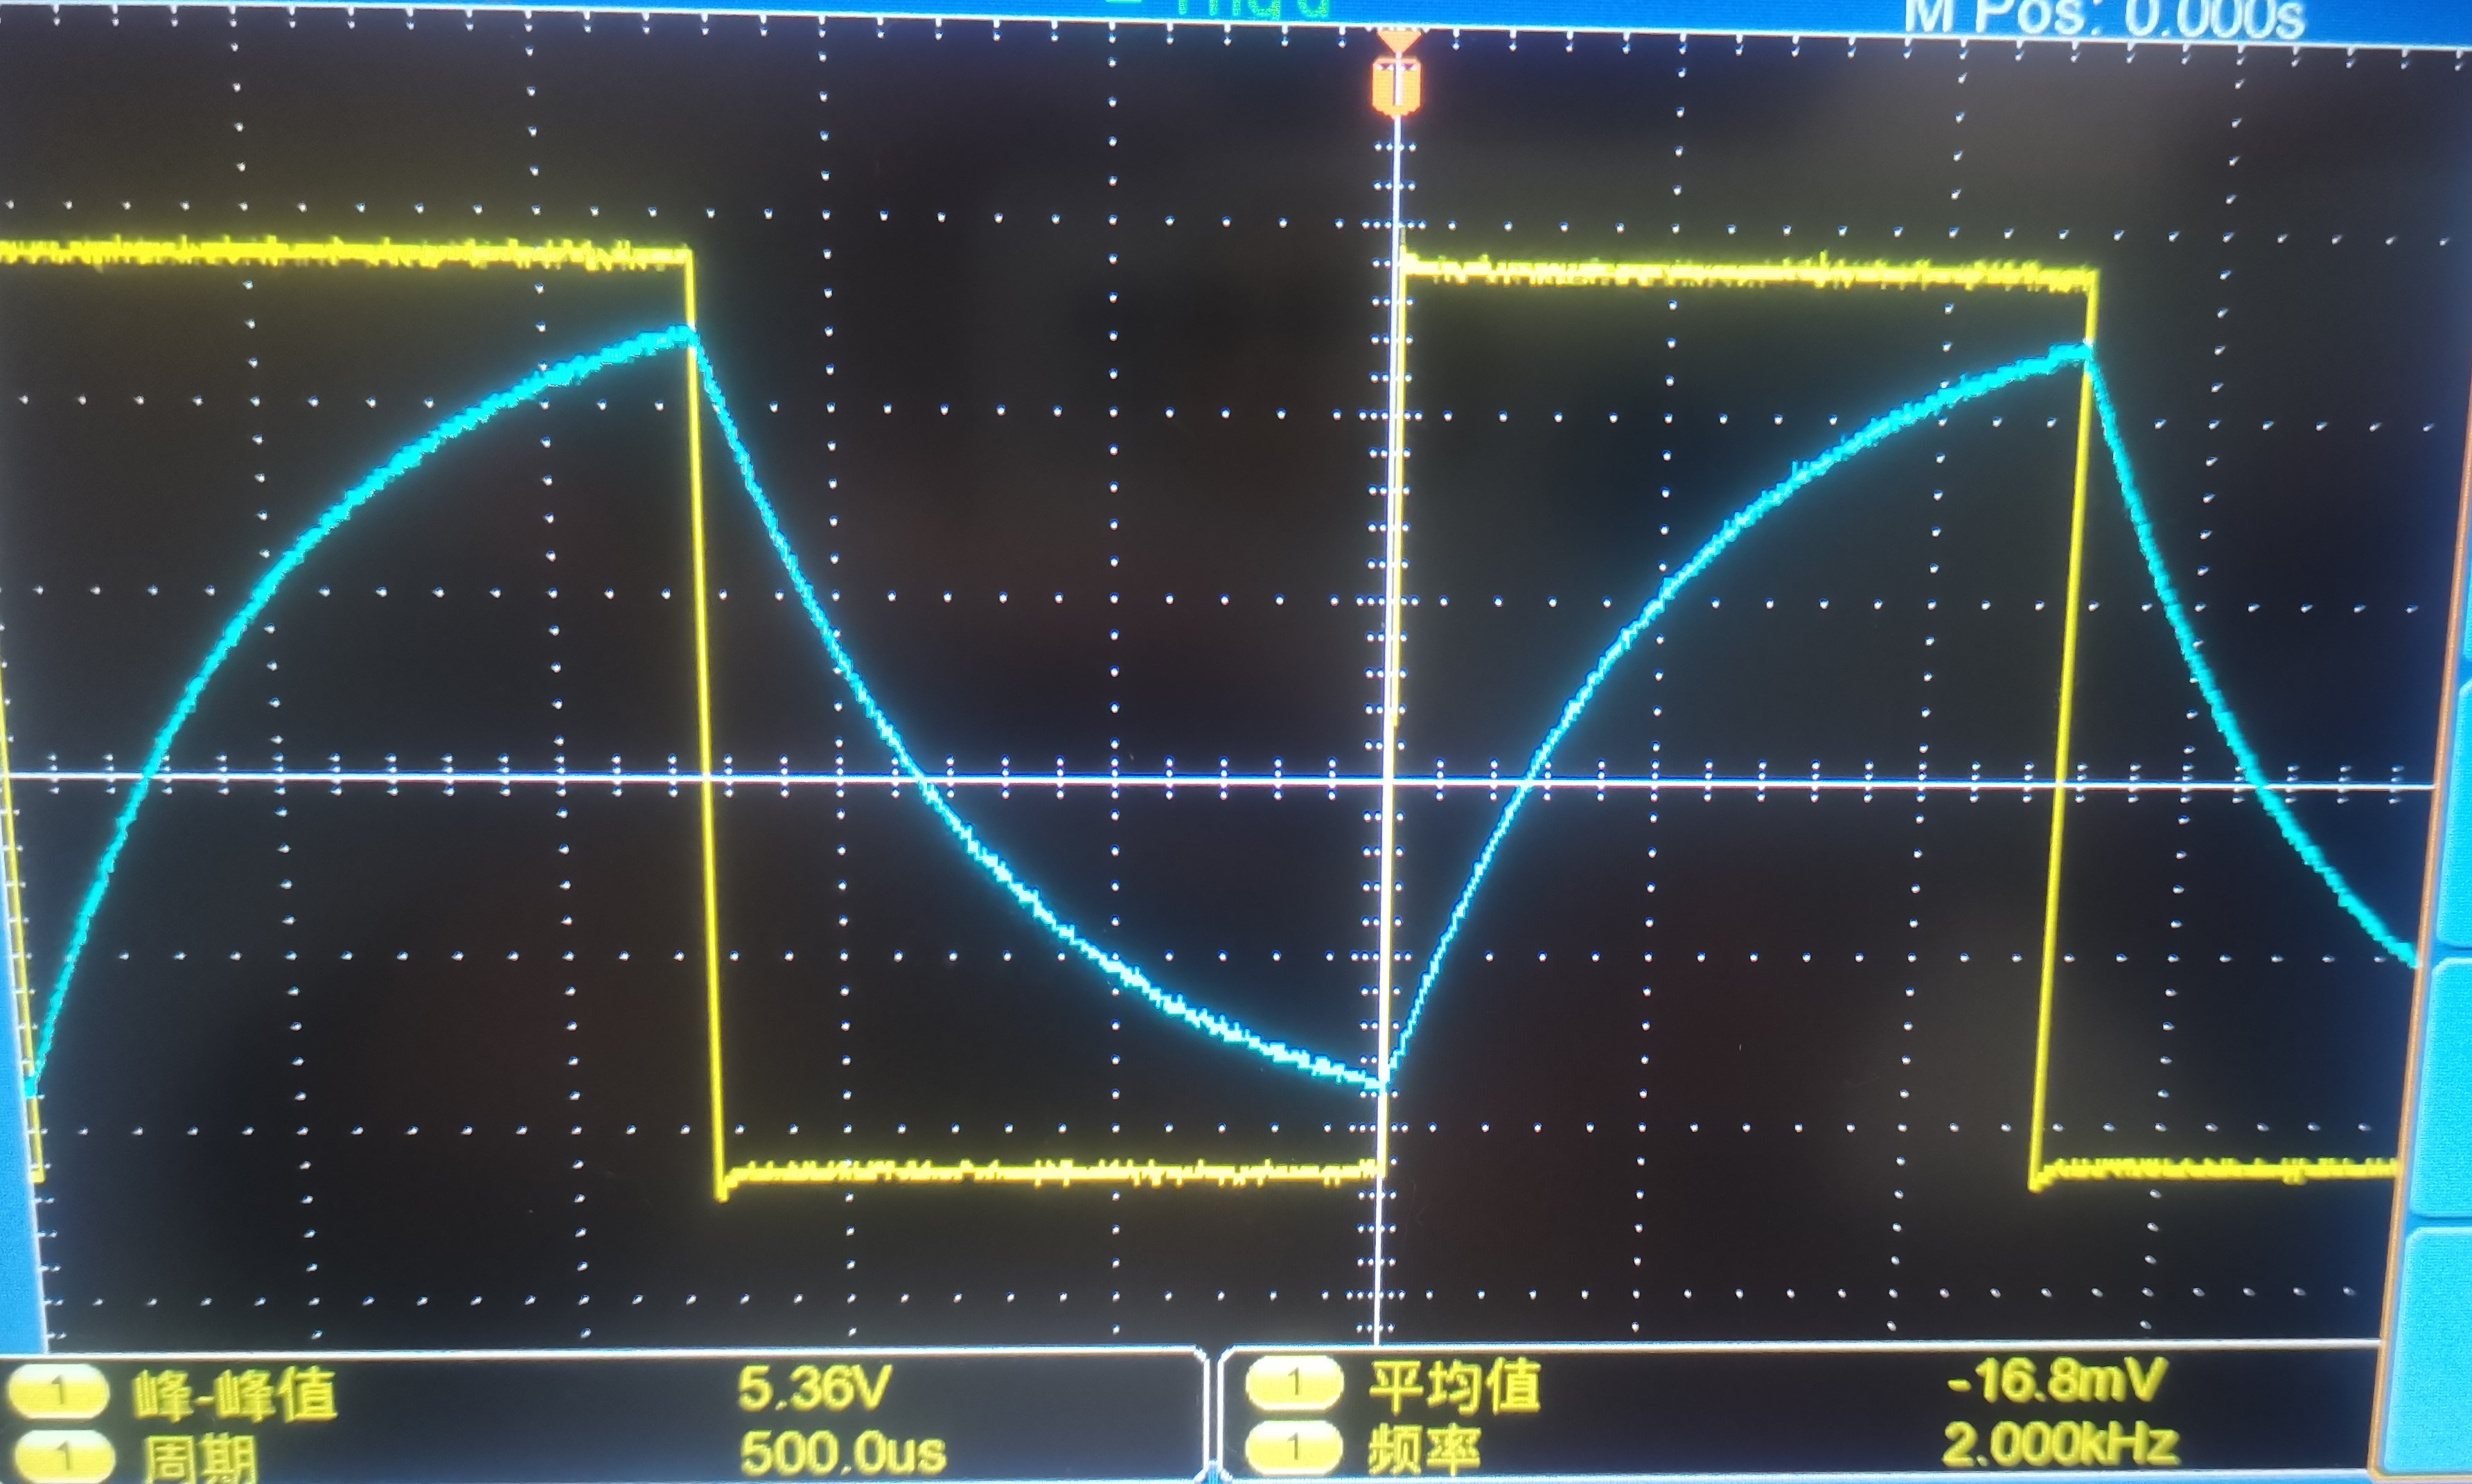
\includegraphics[width=1.9in]{2khz.jpg}
    }
    \quad   
    \subfigure[$f=4kHz$]{
    	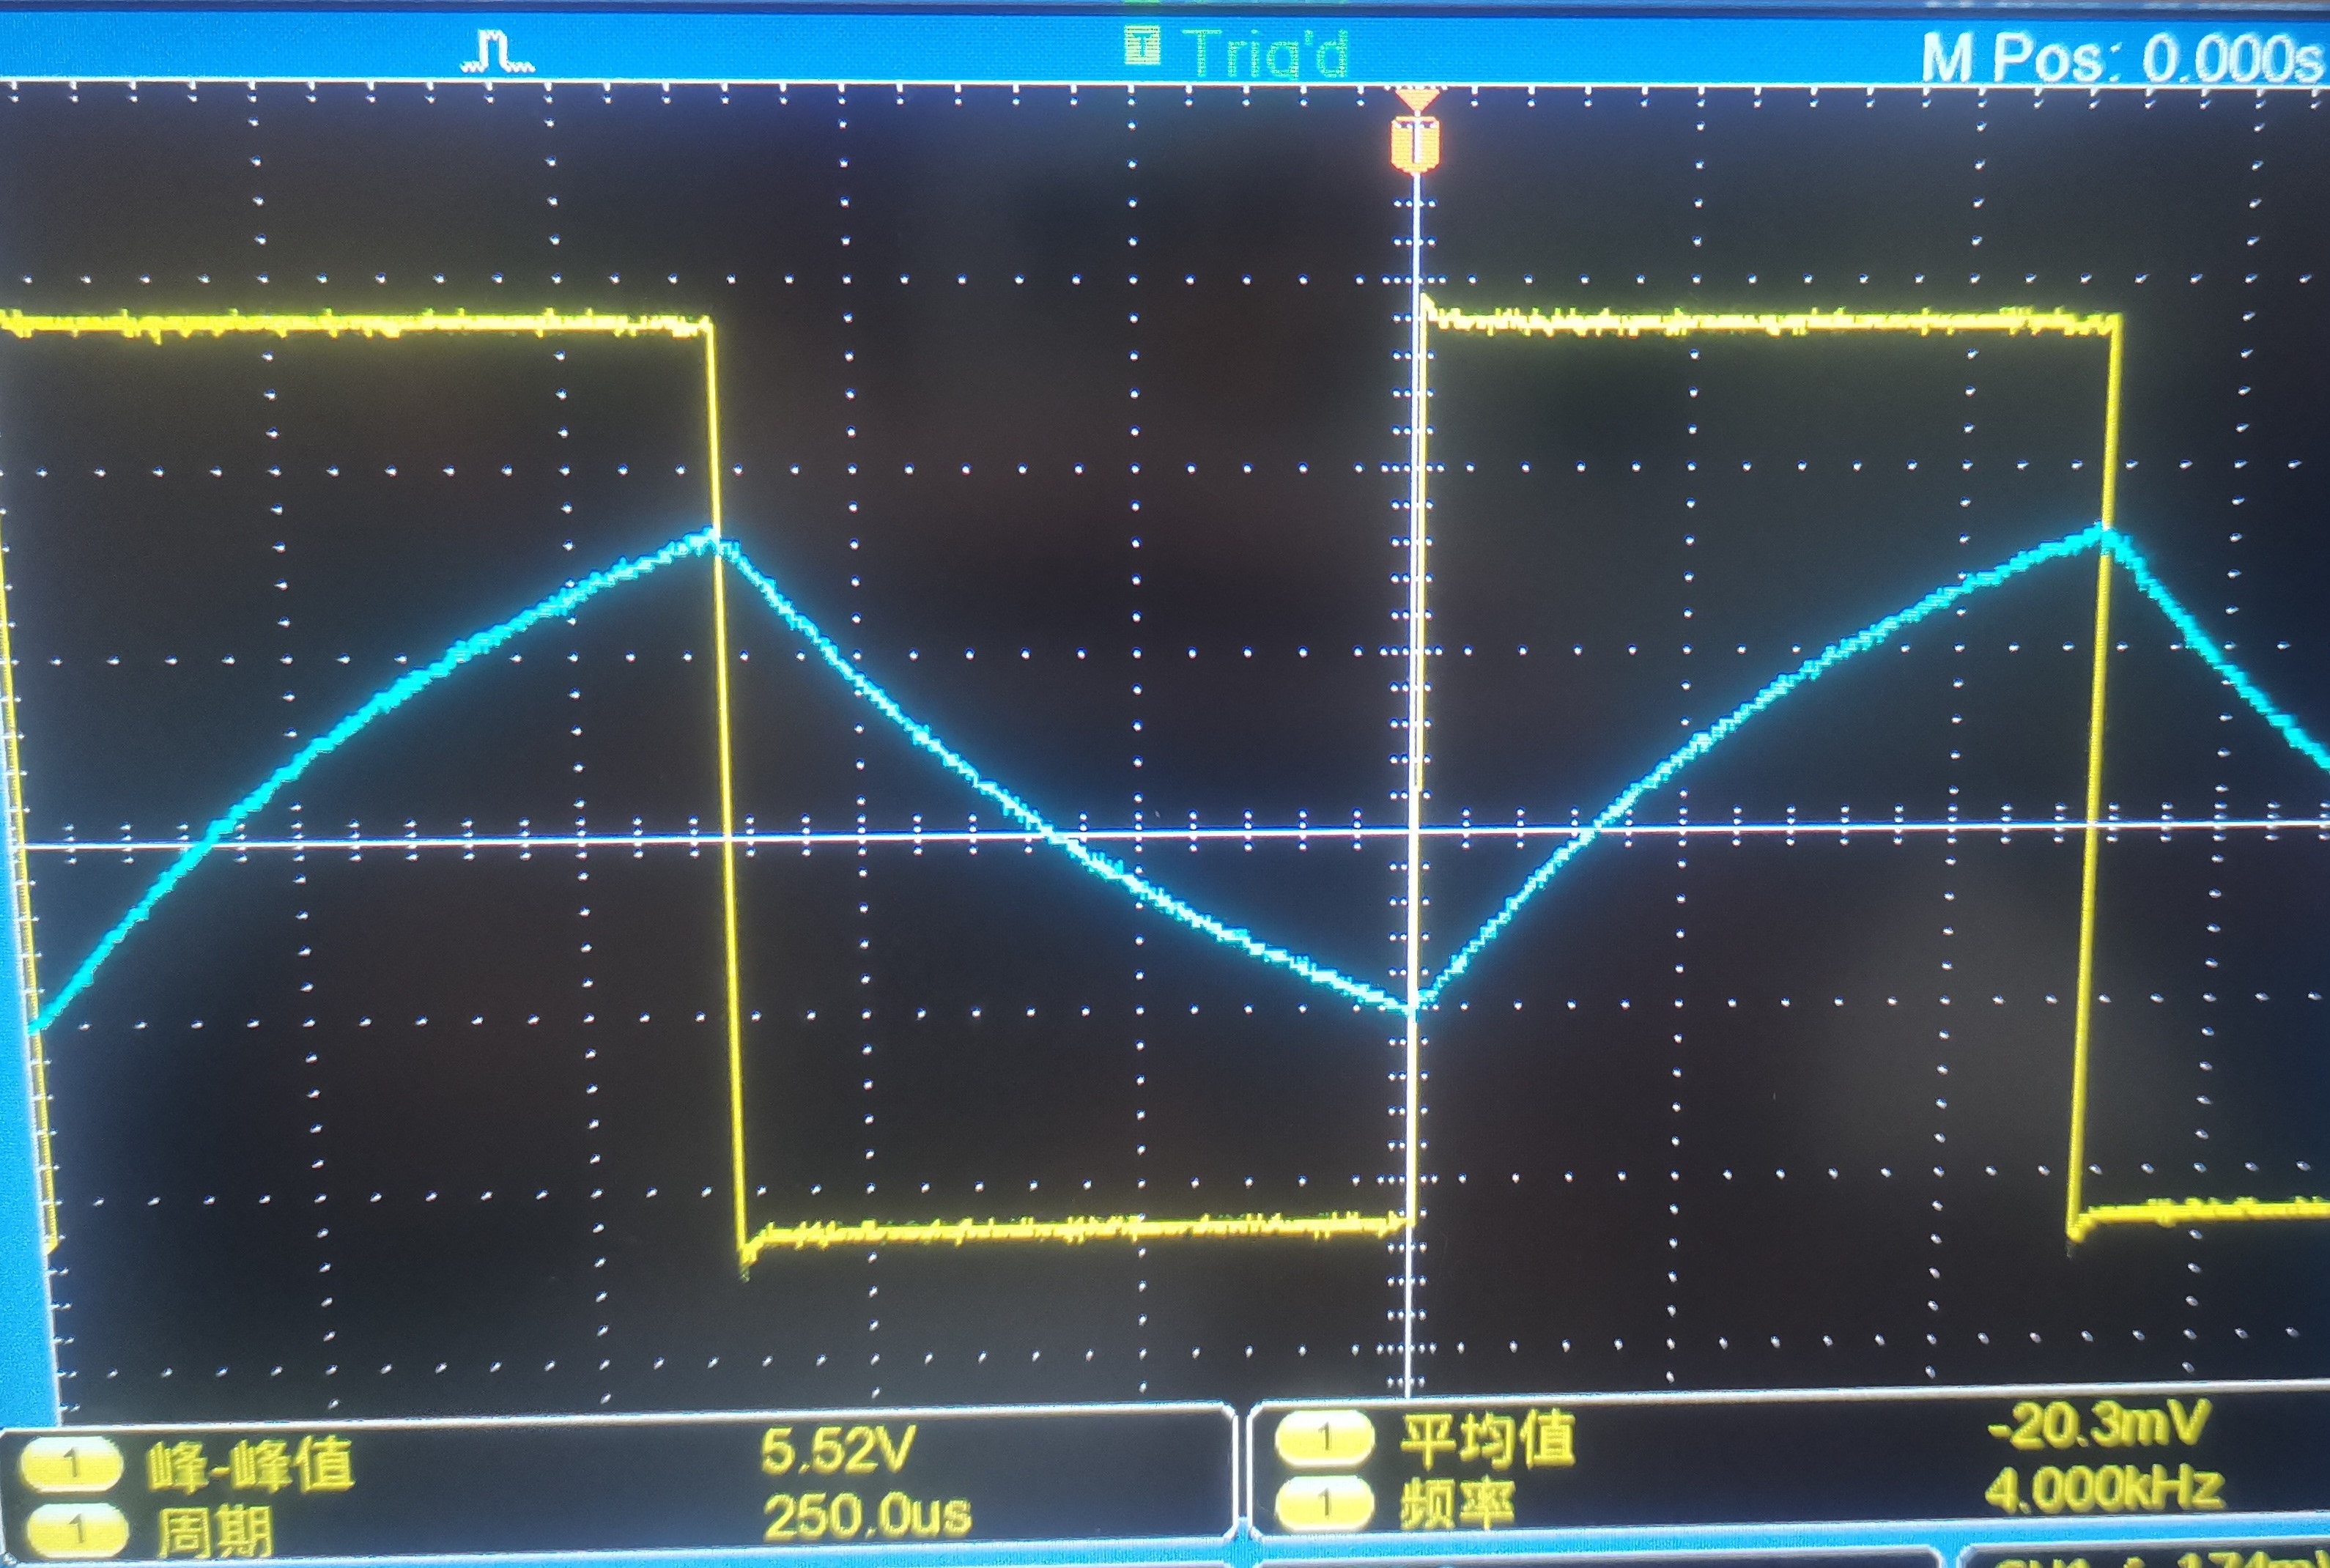
\includegraphics[width=1.9in]{4khz.jpg}
    }
    \subfigure[$f=8kHz$]{
	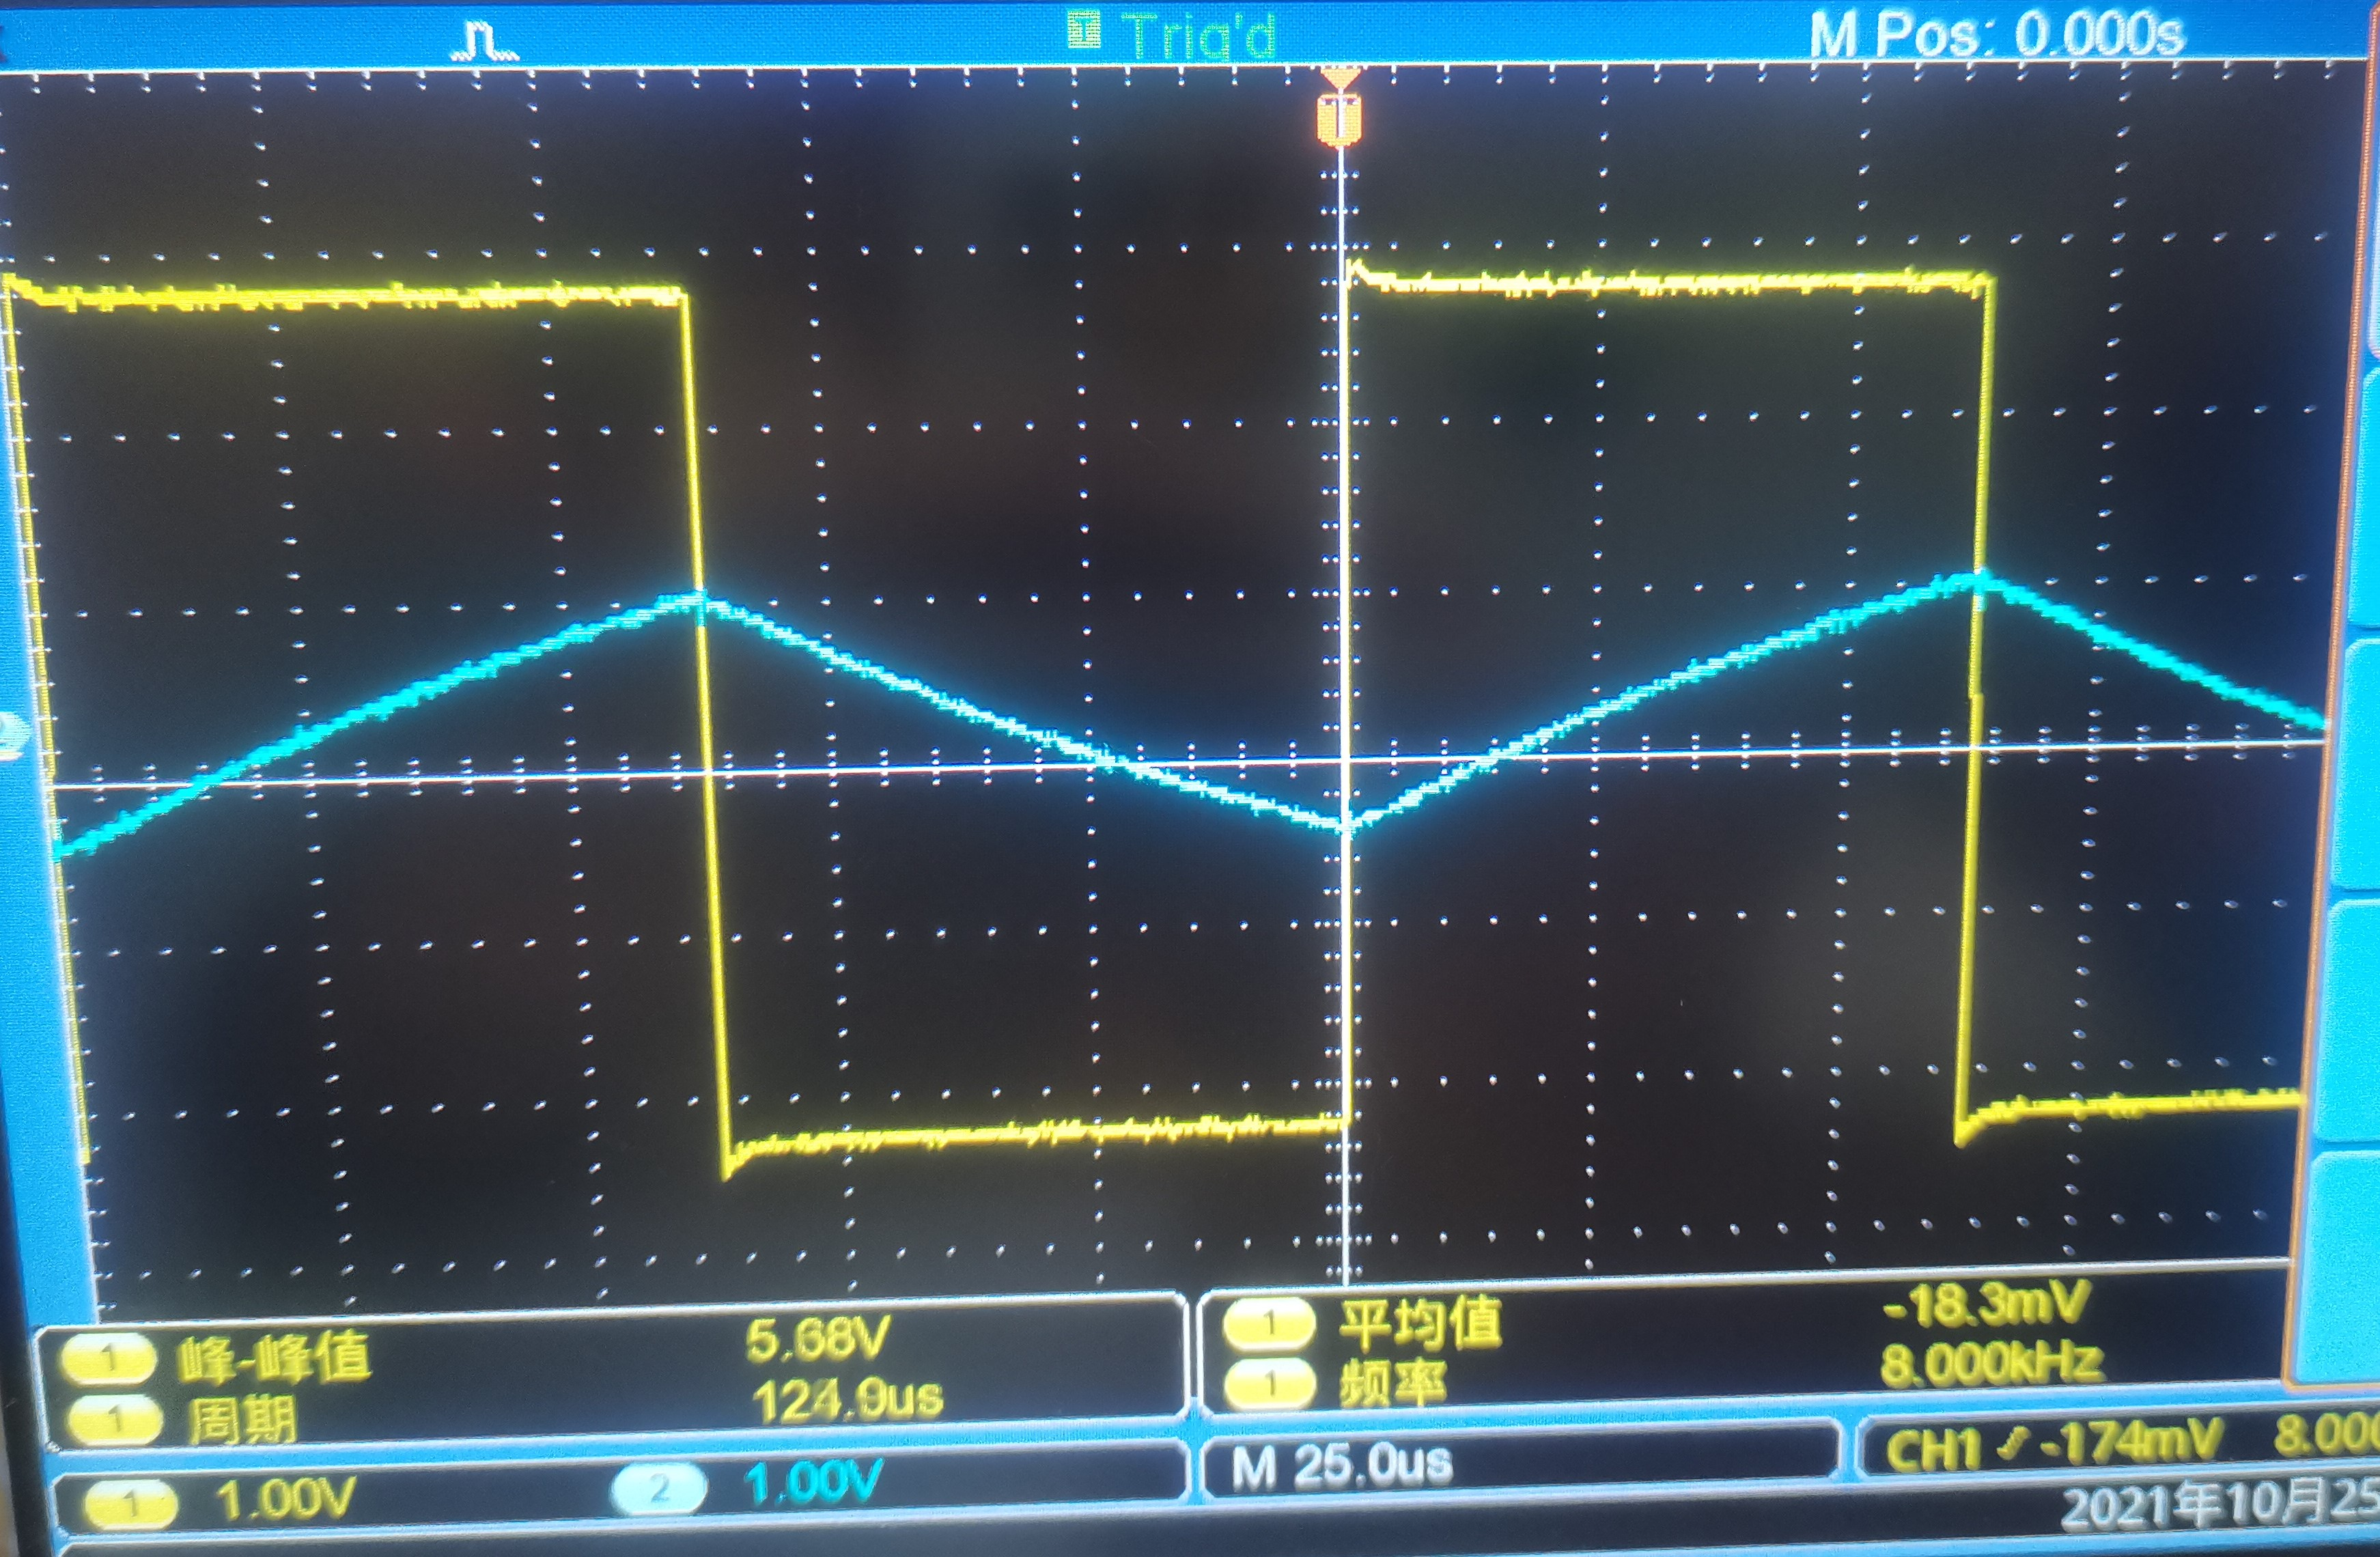
\includegraphics[width=1.9in]{8khz.jpg}
    }
    \caption{$R=10k \Omega$ , 逐渐增大f}
    \label{fig.1}
\end{figure}

根据公式 $ u_{c}=E\left(1-e^{\frac{-t}{R C}}\right) $ 可知, 当增大  R  或增大  f  (减小T), $ u_{c} $ 的幅值均会减小。

观察可知当电阻R增大或频率f增大时, 产生的波形更接近于三角波, 但电路的输出幅度会减小,与理论符合。
这是由于电容通过电阻充放电, 在相对于时间常数  $\tau=R C  $很小的时间段内($3-5\tau$ 远大于周期), 波形变化接近线性。
因此,通过增大 RC 电路的  $\tau$  或通过增大频率  f  减小充放电时间  t  均可以使波形变化更接近线性, 从而产生近似的三角波。
\subsubsection{尖脉冲产生原理研究}

初始条件:$f=1kHz,R=200\Omega,C=10.435nF$

\begin{figure}[htbp]
    \centering
    \subfigure[$f=1kHz$]{
        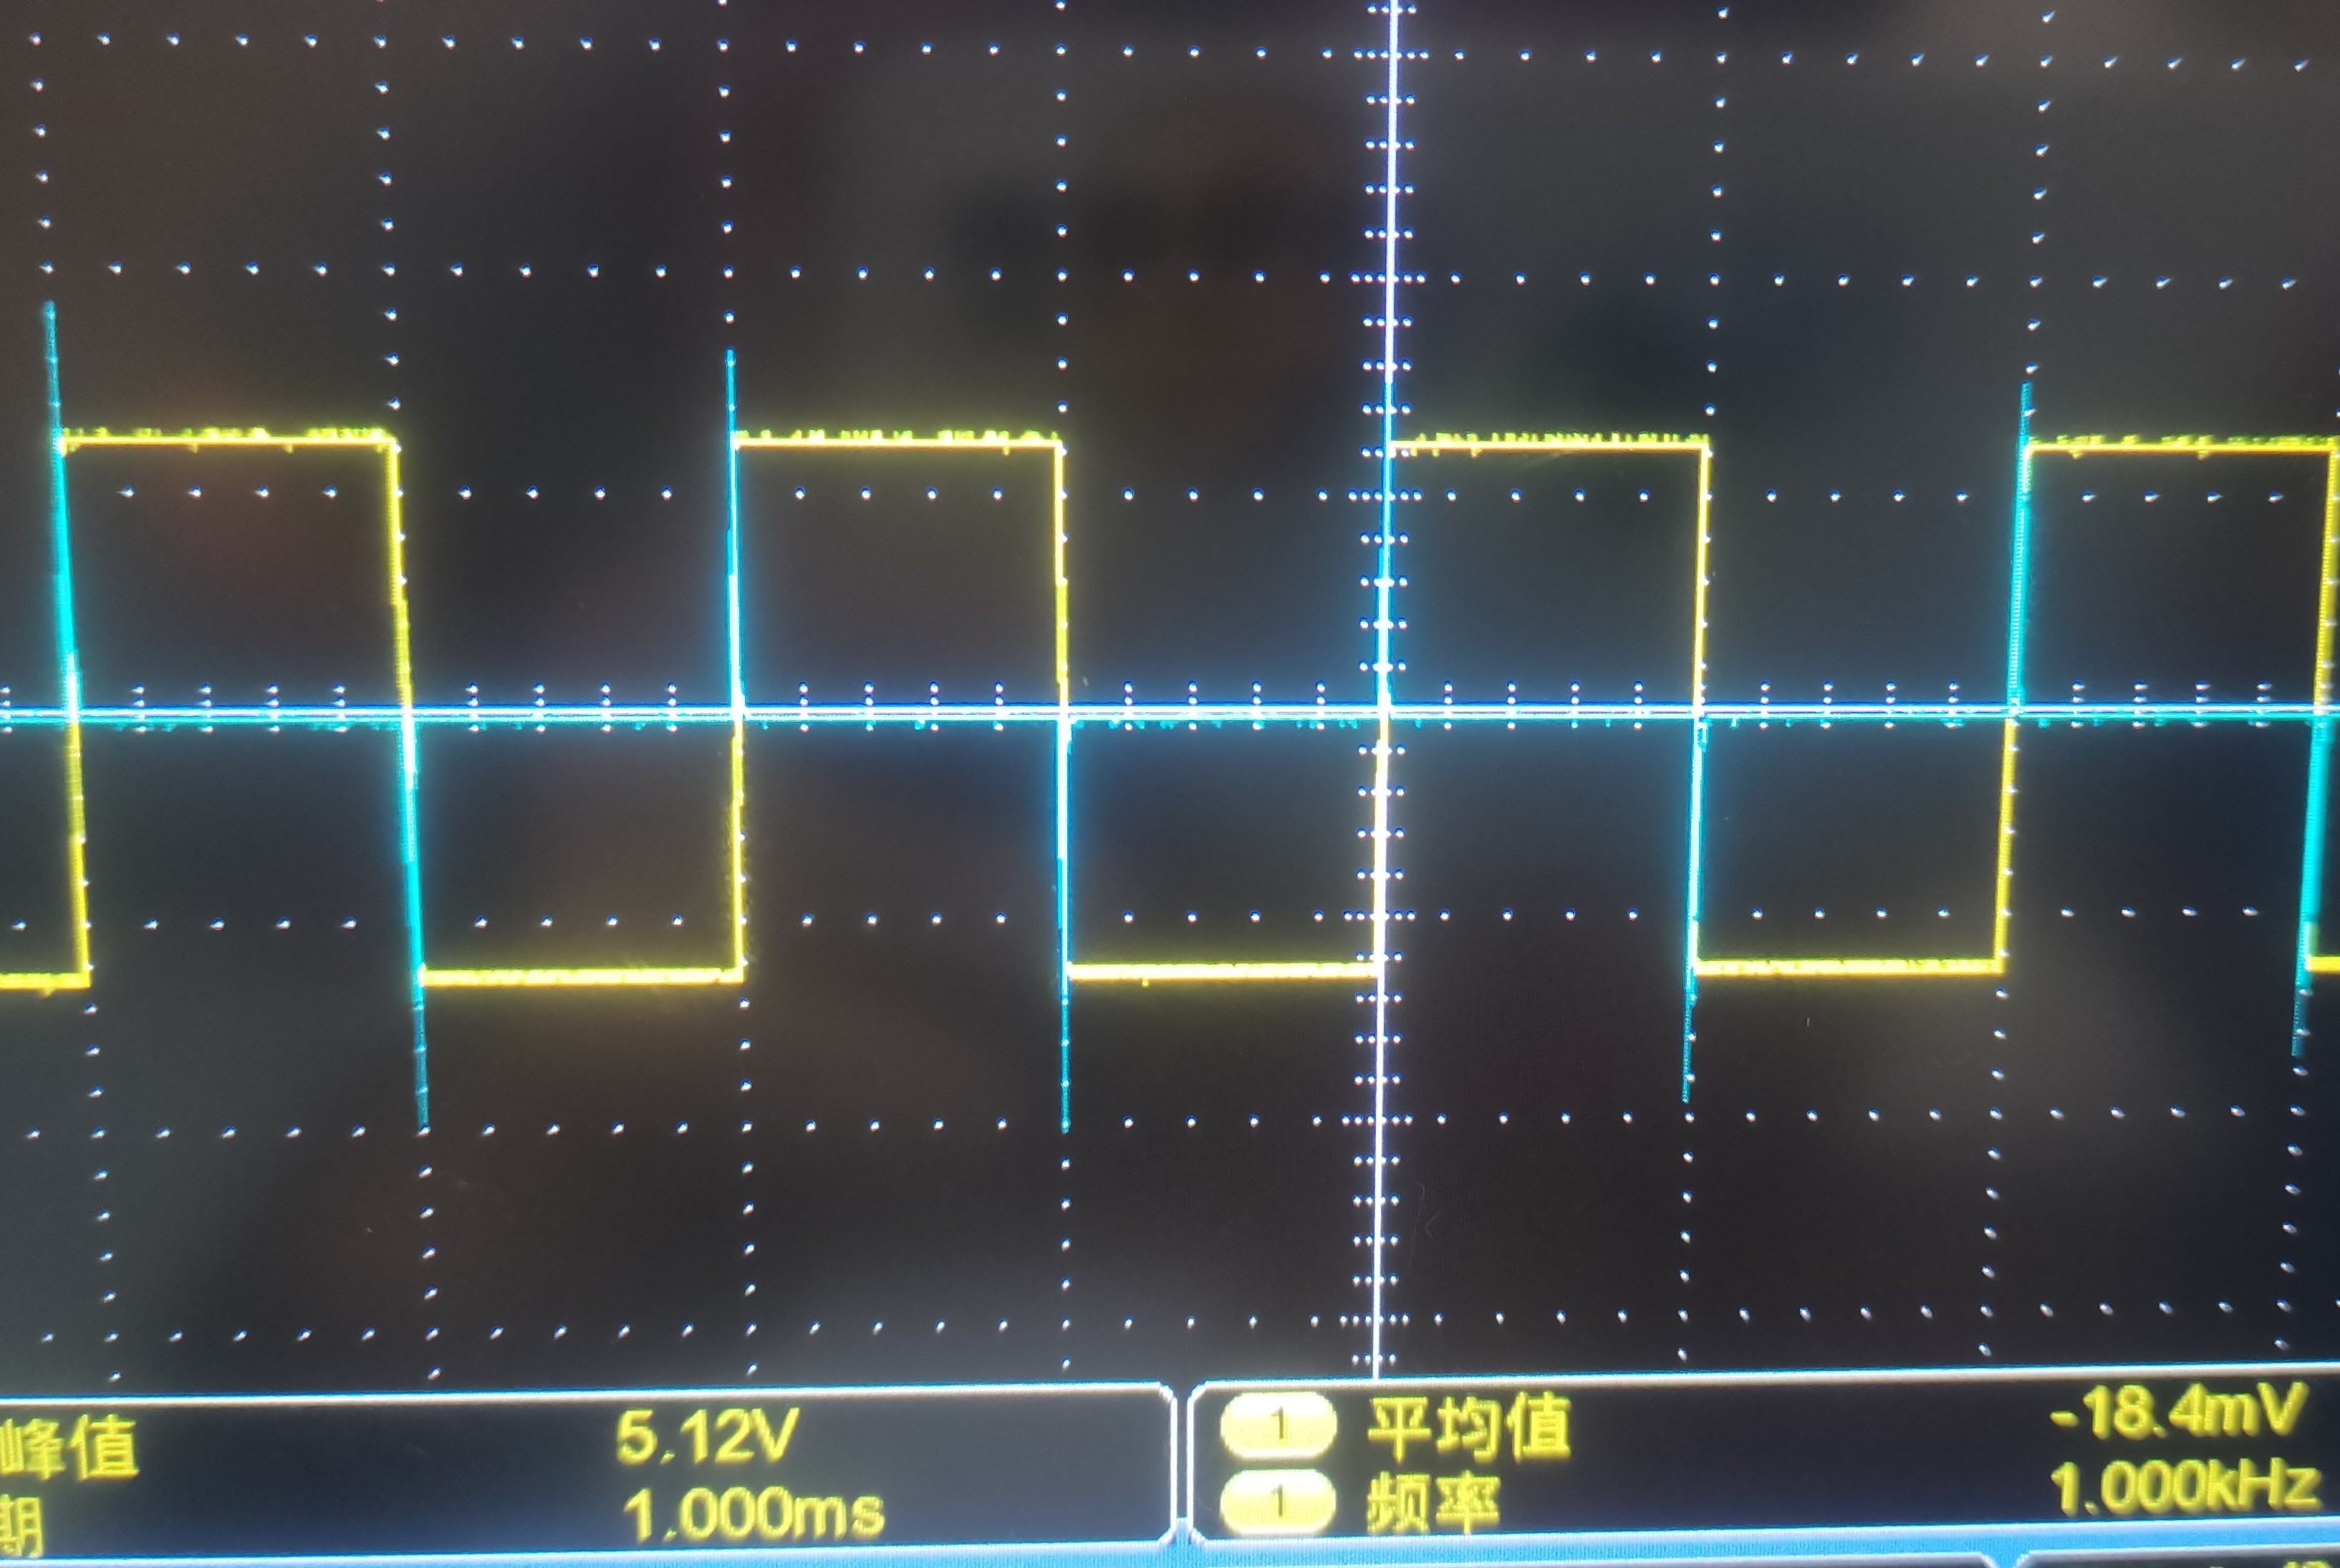
\includegraphics[width=1.8in]{200O.jpg}
    }
    \subfigure[$f=2kHz$]{
	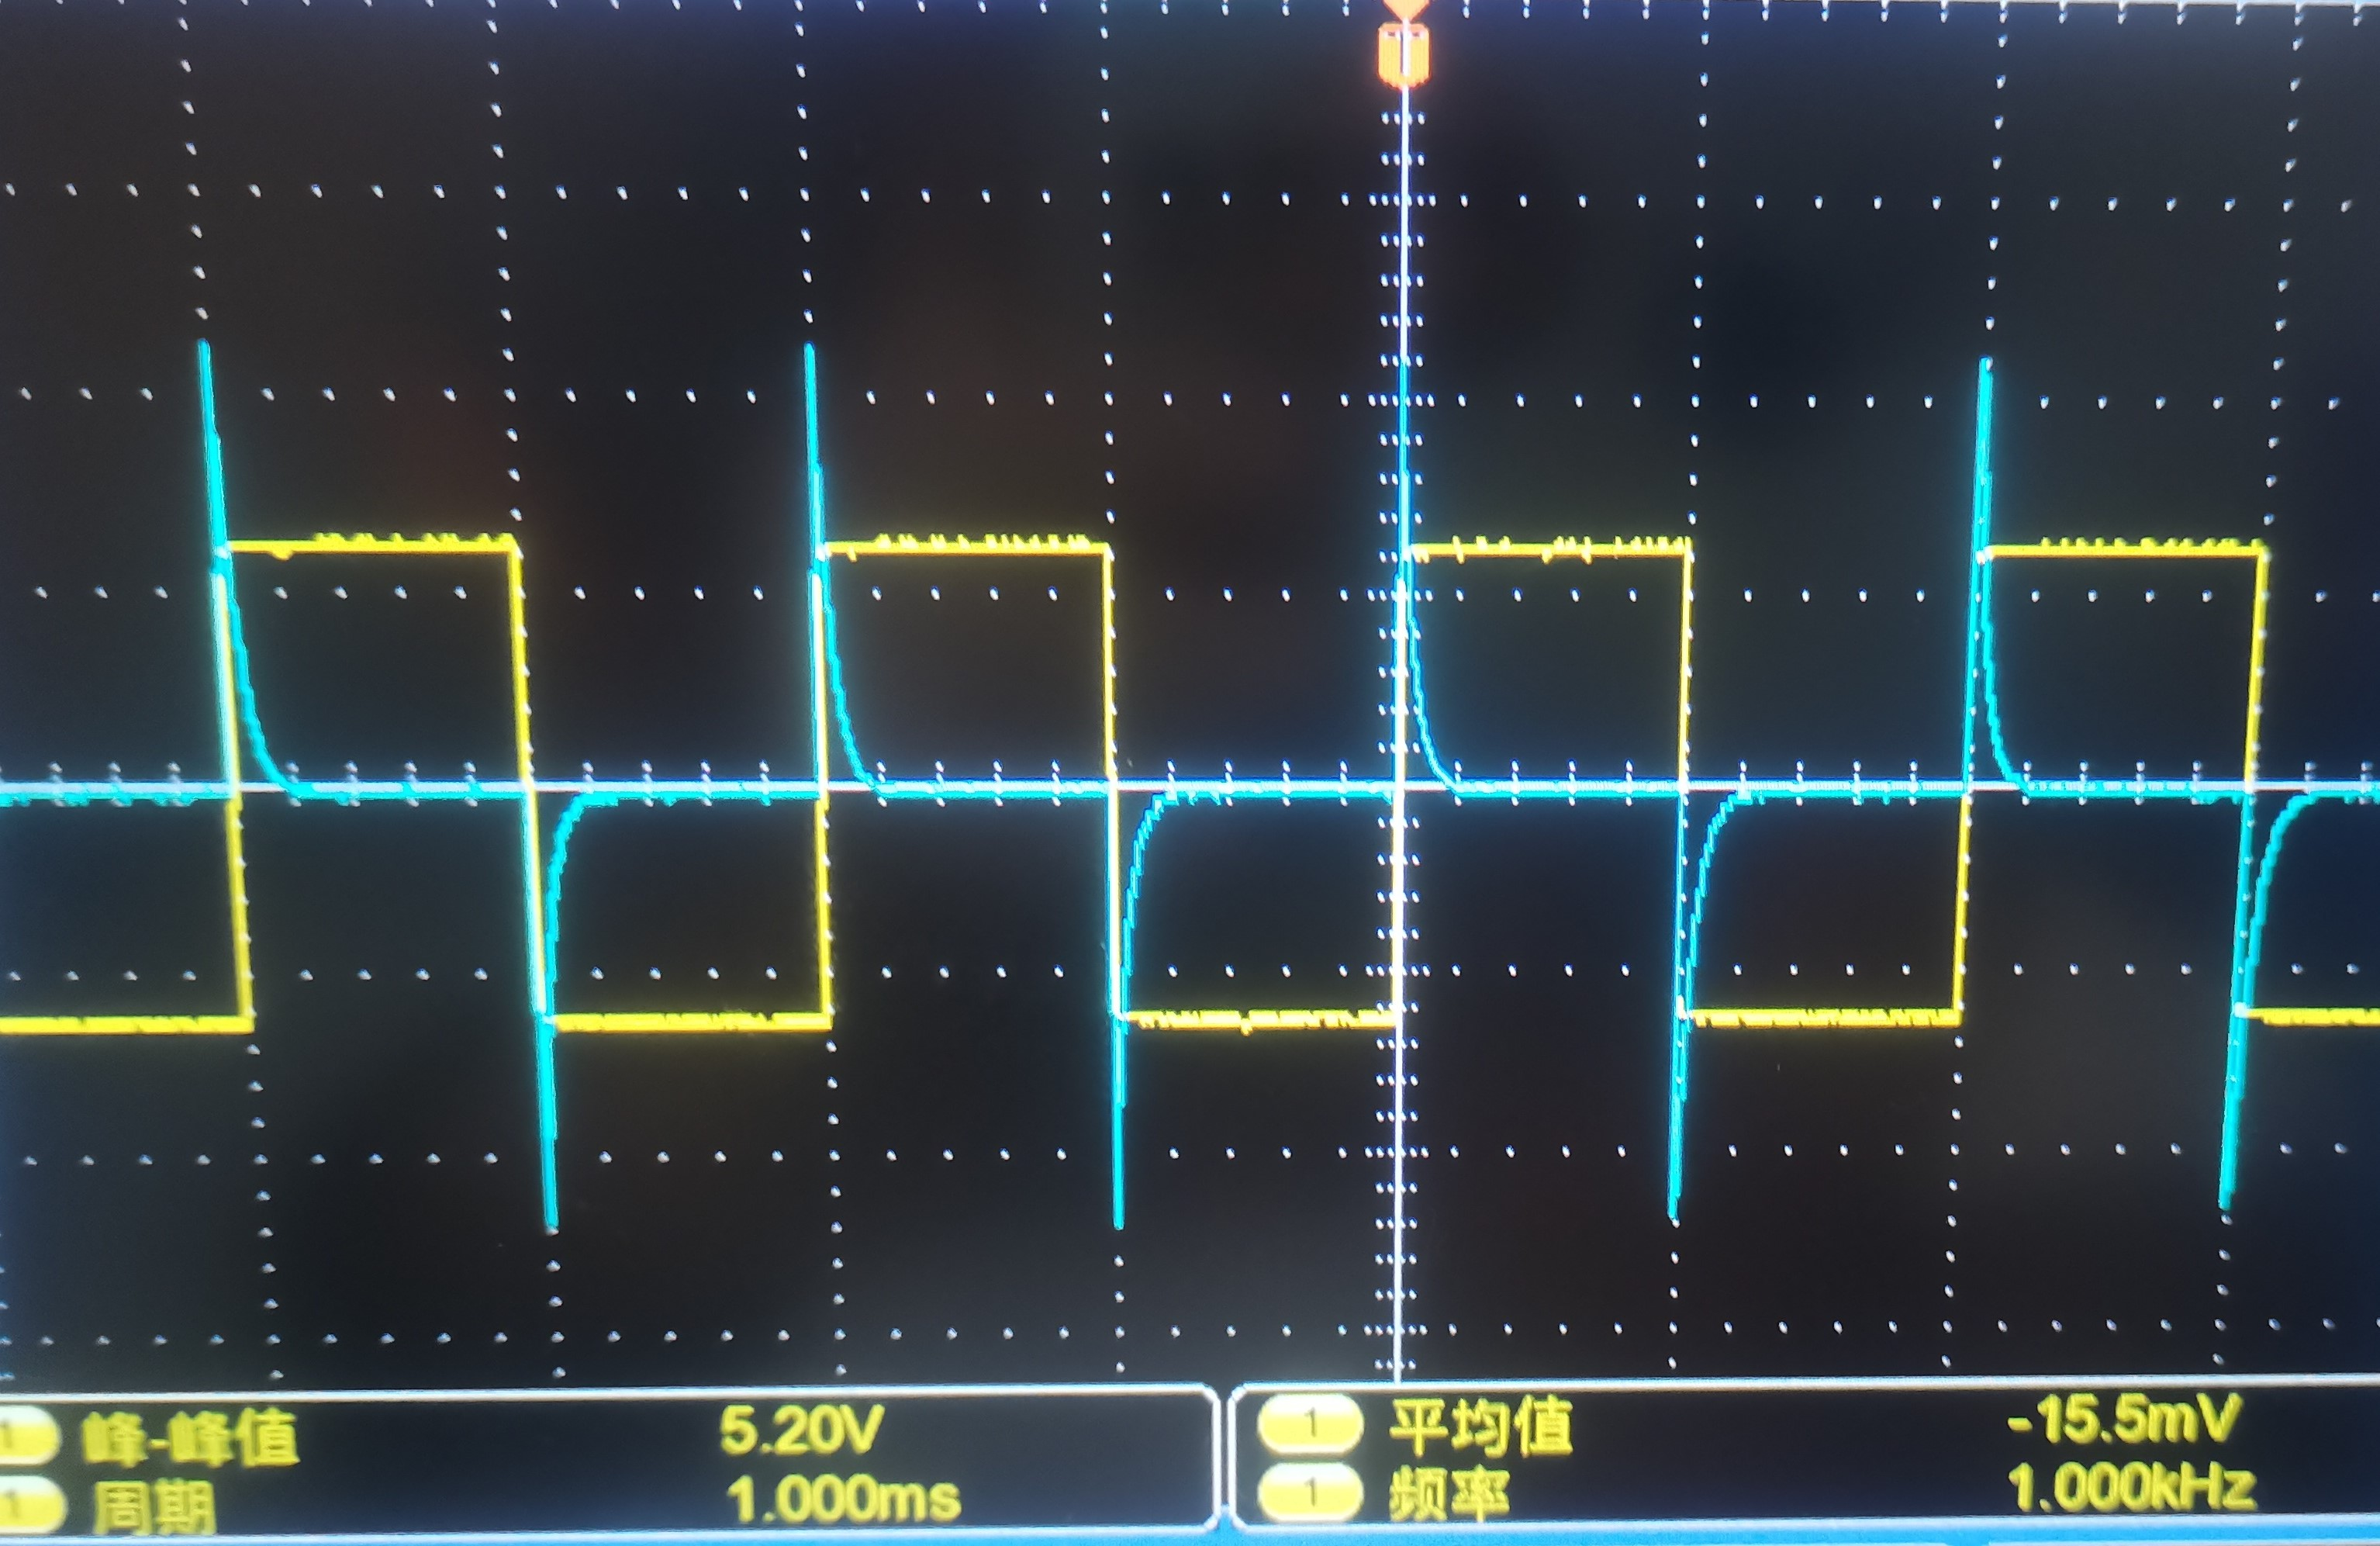
\includegraphics[width=1.8in]{2kO.jpg}
    }
    \quad   
    \subfigure[$f=4kHz$]{
    	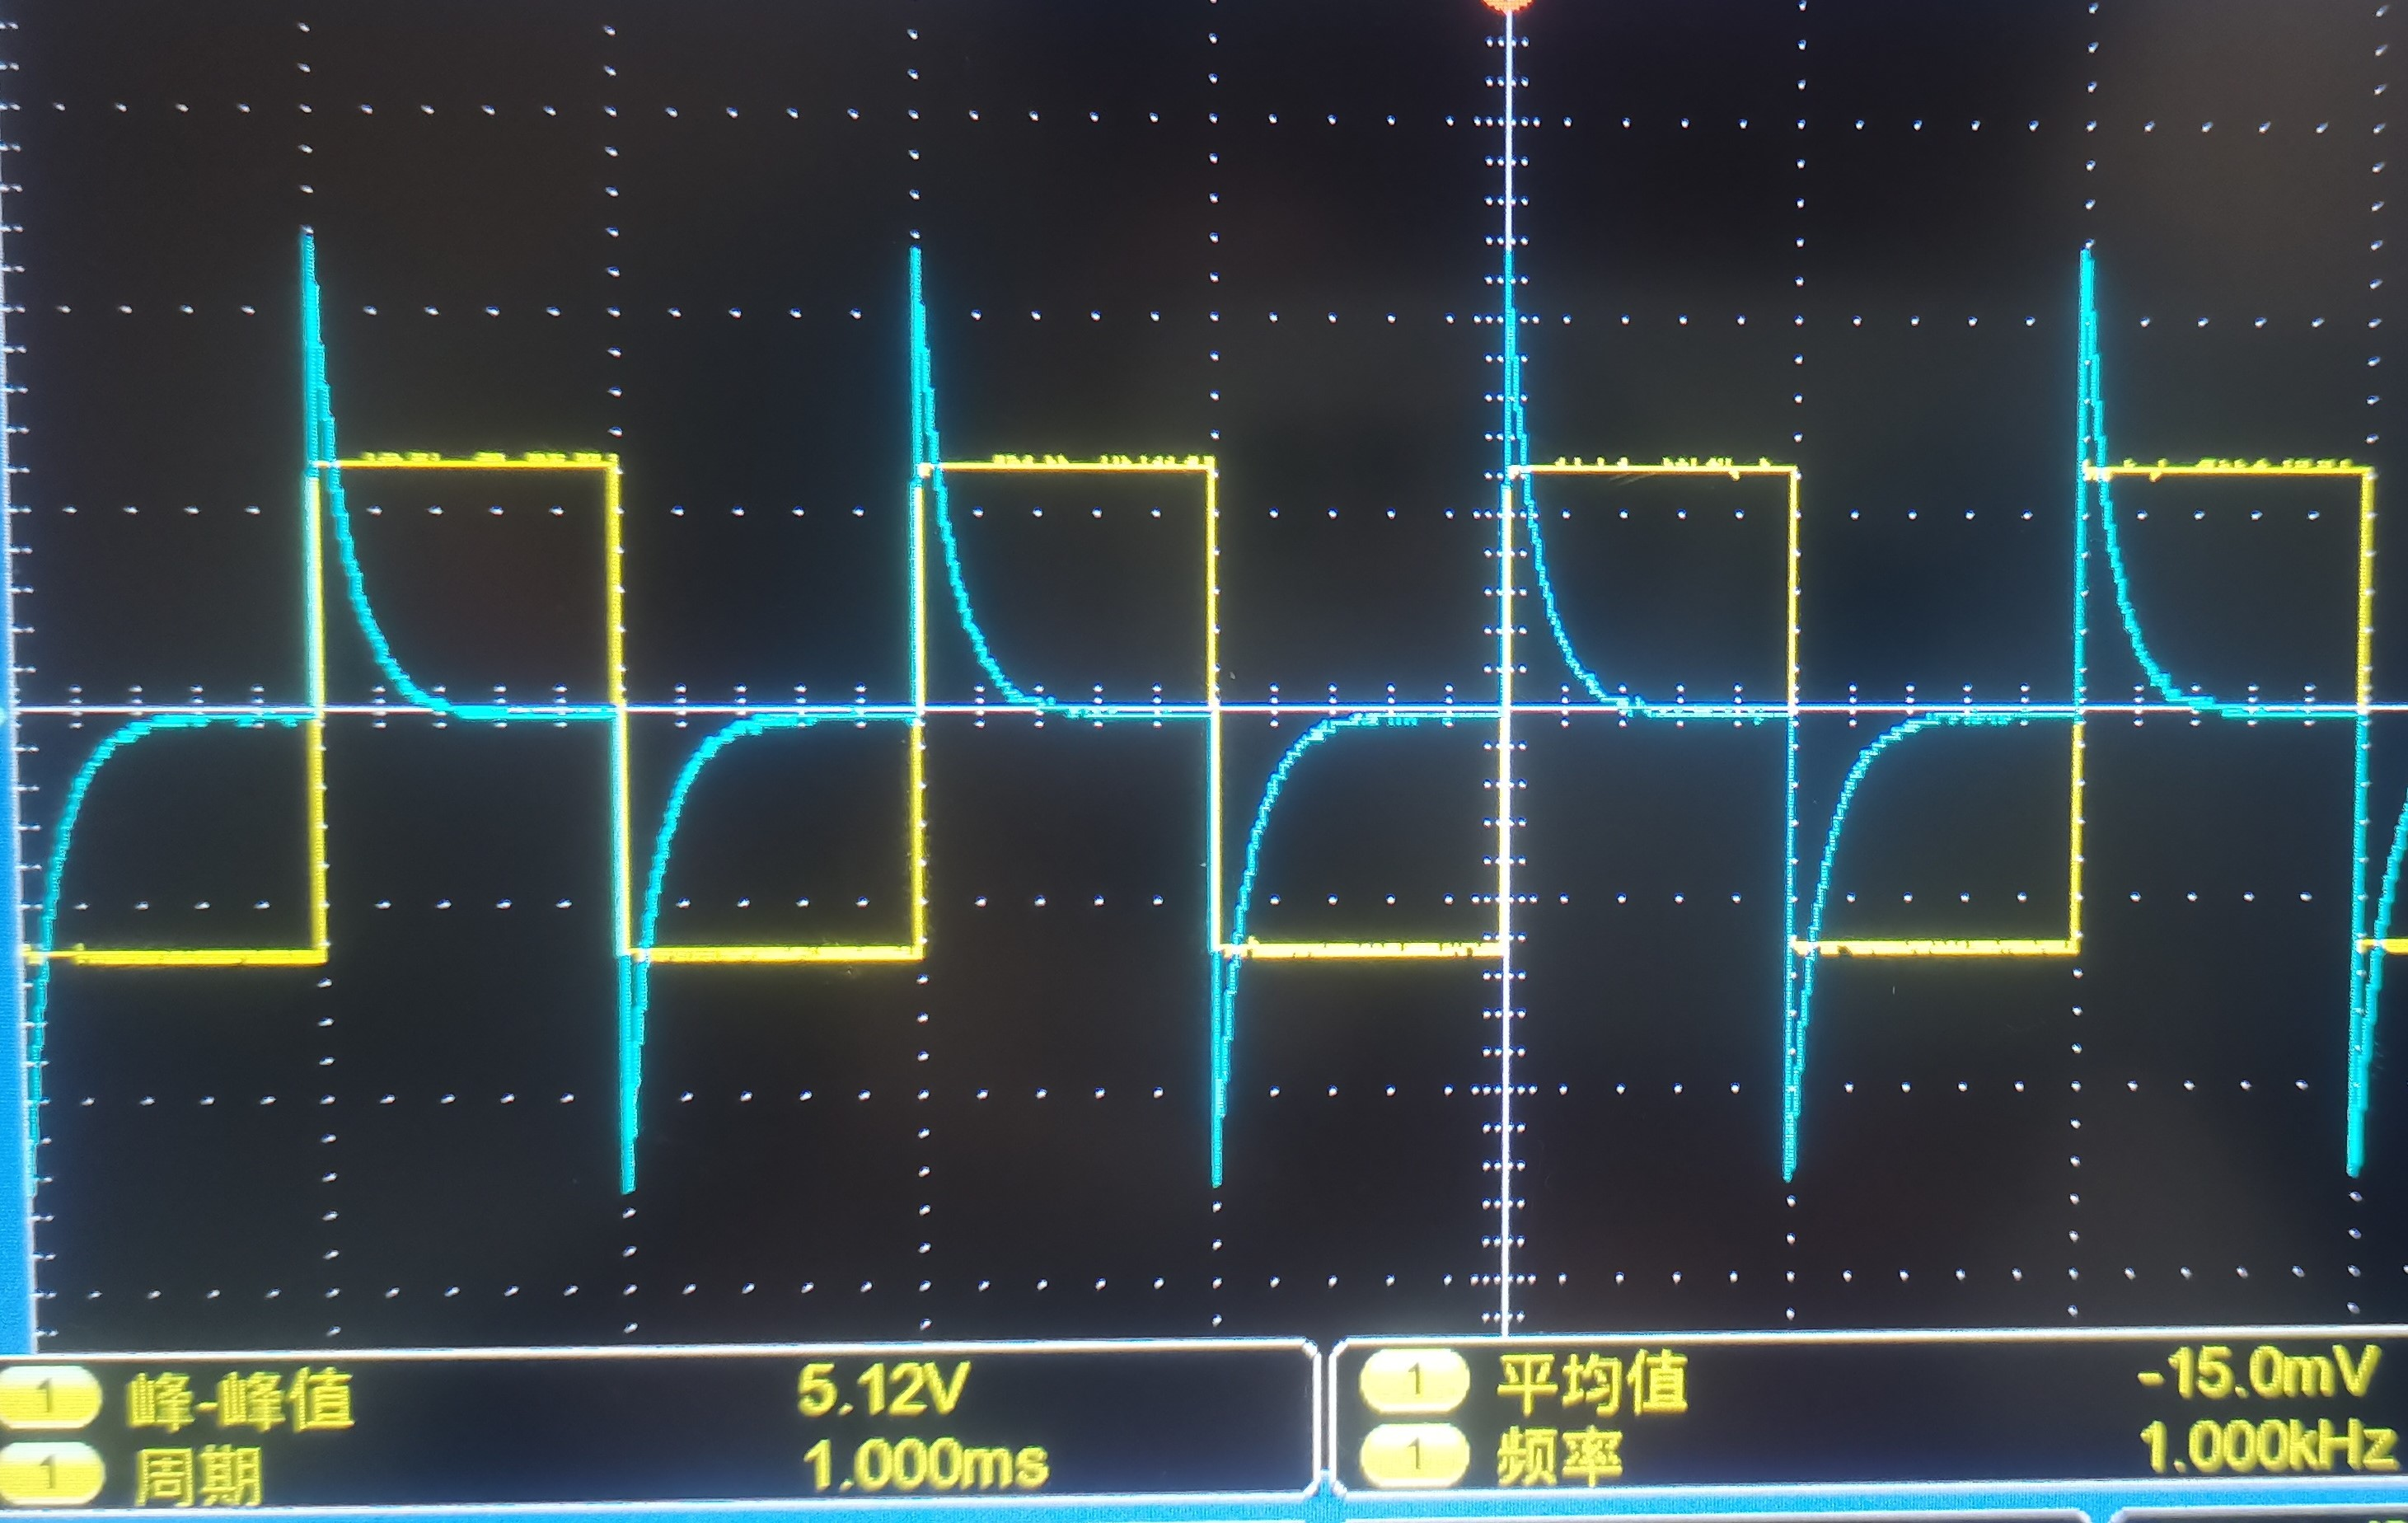
\includegraphics[width=1.8in]{5kO.jpg}
    }
    \caption{$f=1kHz$ , 逐渐增大R}
    \label{fig.1}
\end{figure}

\begin{figure}[htbp]
    \centering
    \subfigure[$f=2kHz$]{
        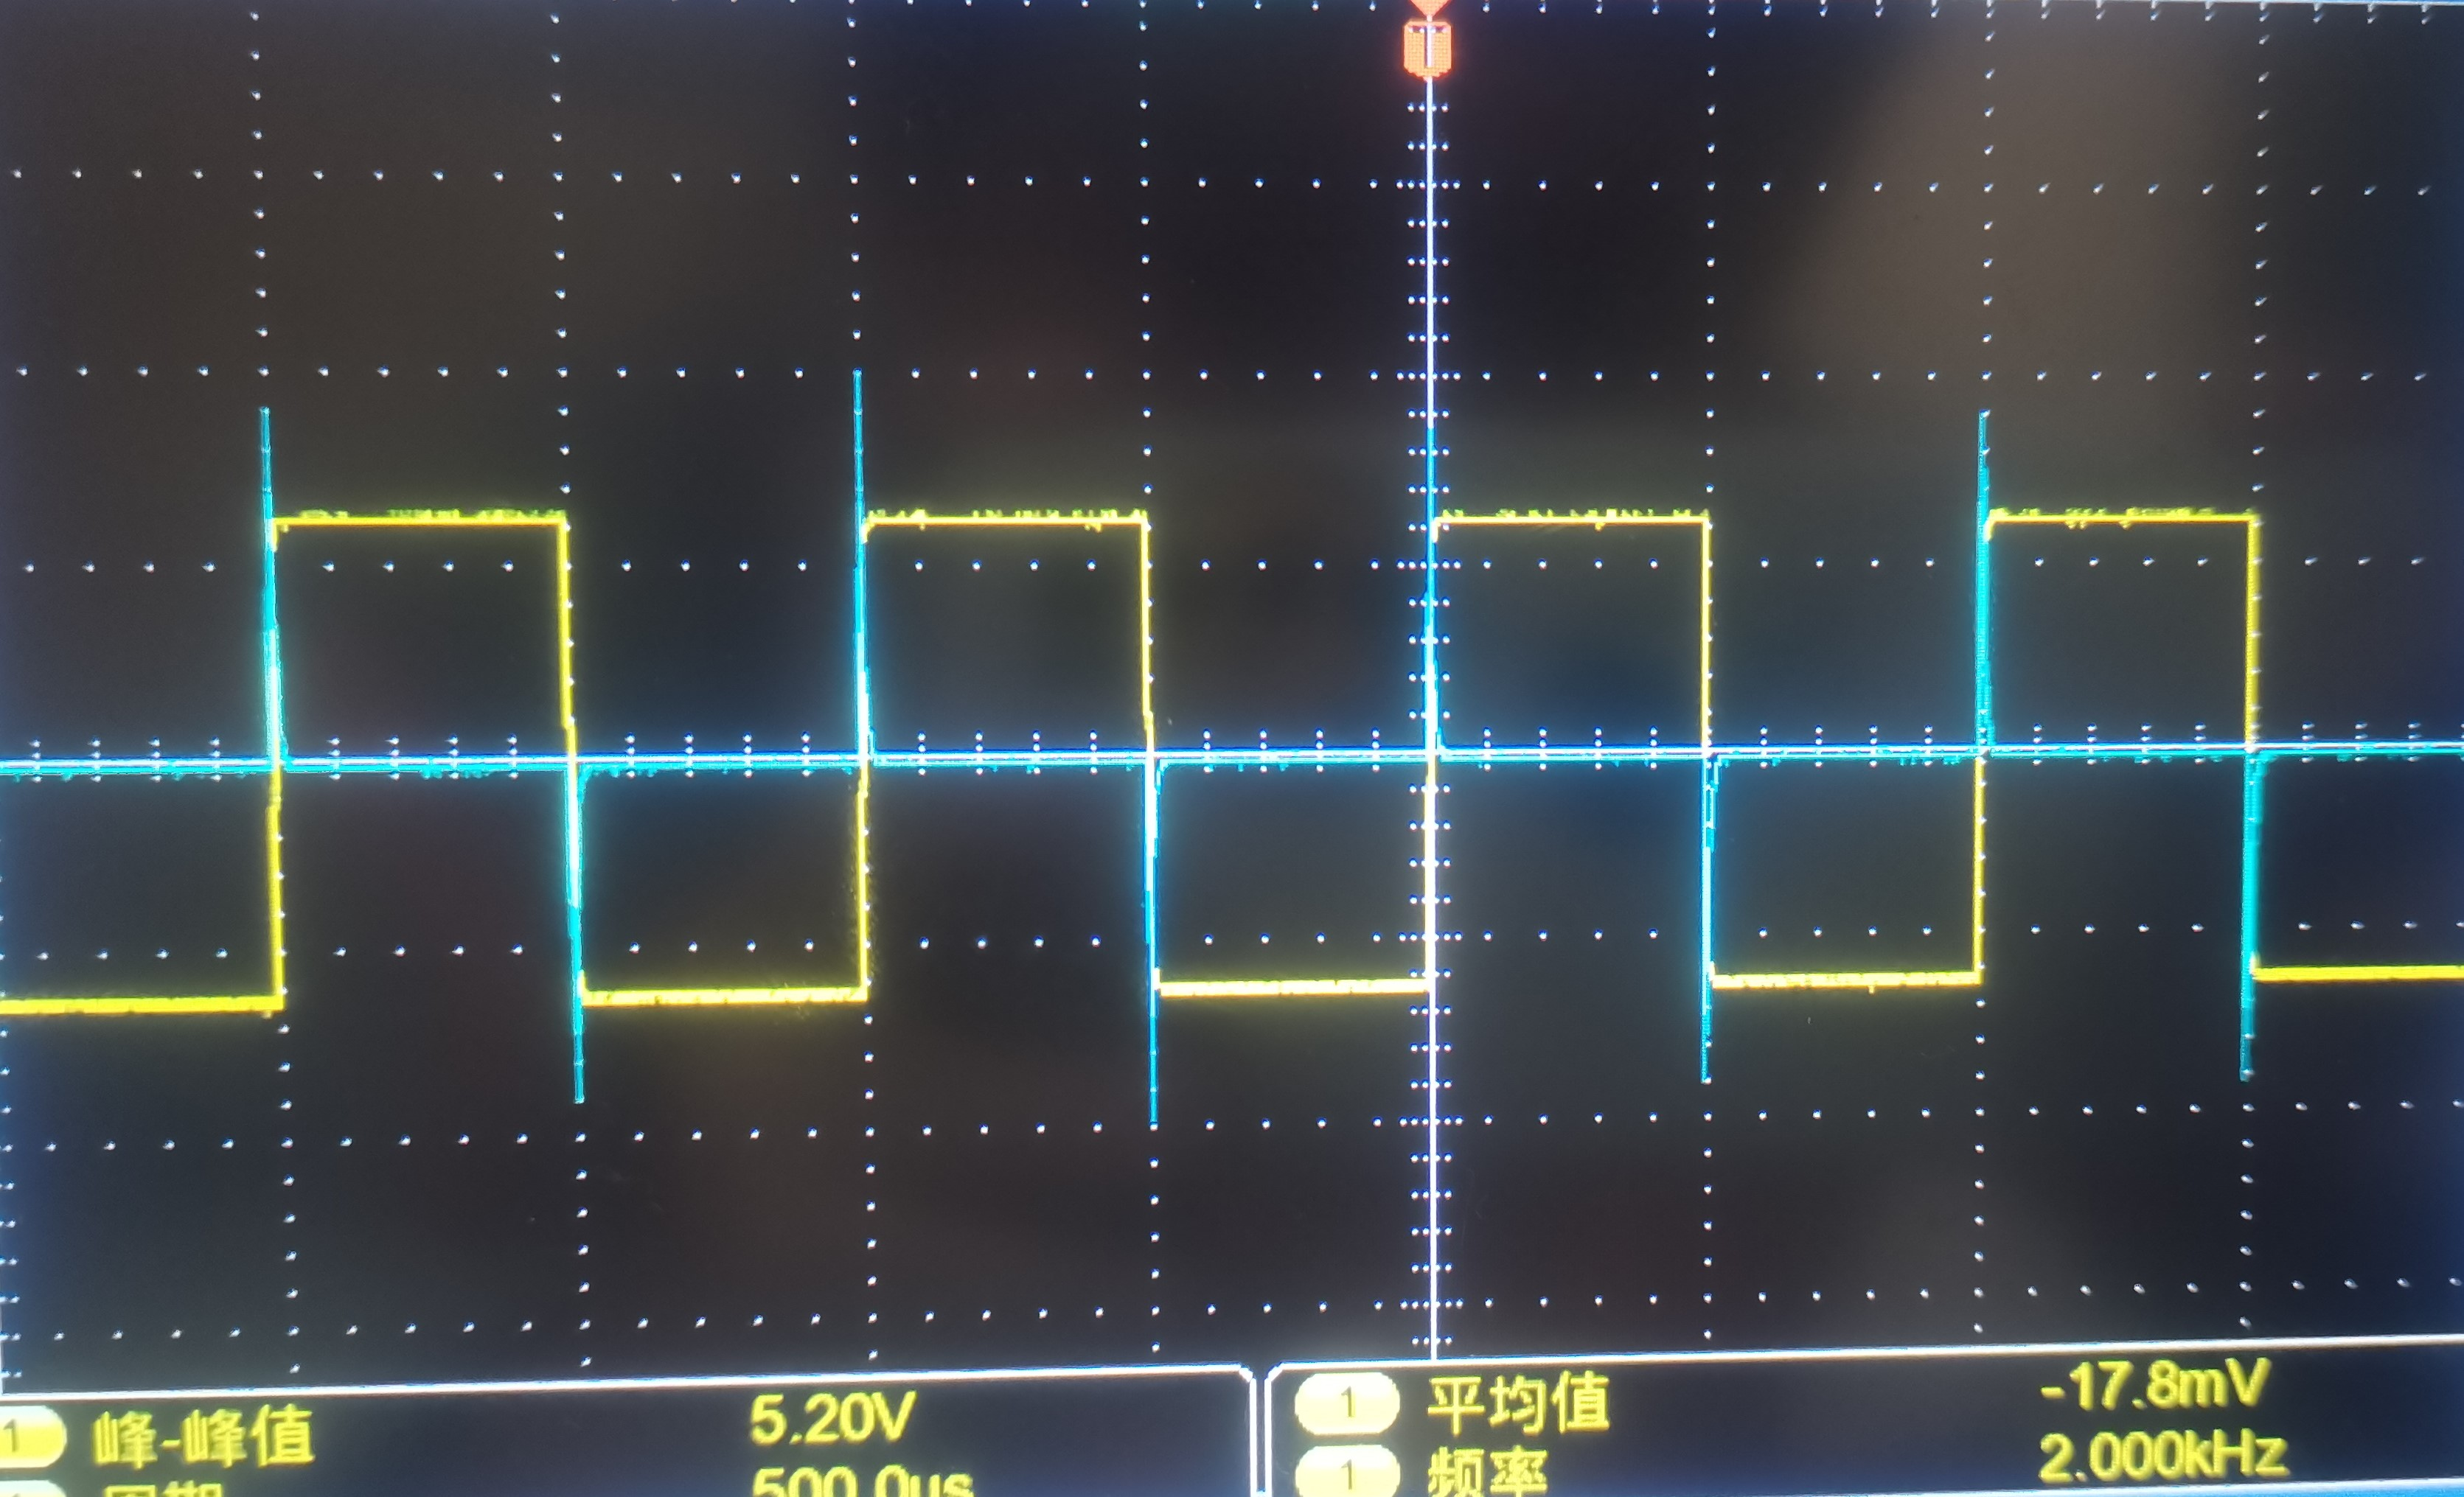
\includegraphics[width=2in]{尖脉冲2k.jpg}
    }
    \subfigure[$f=4kHz$]{
	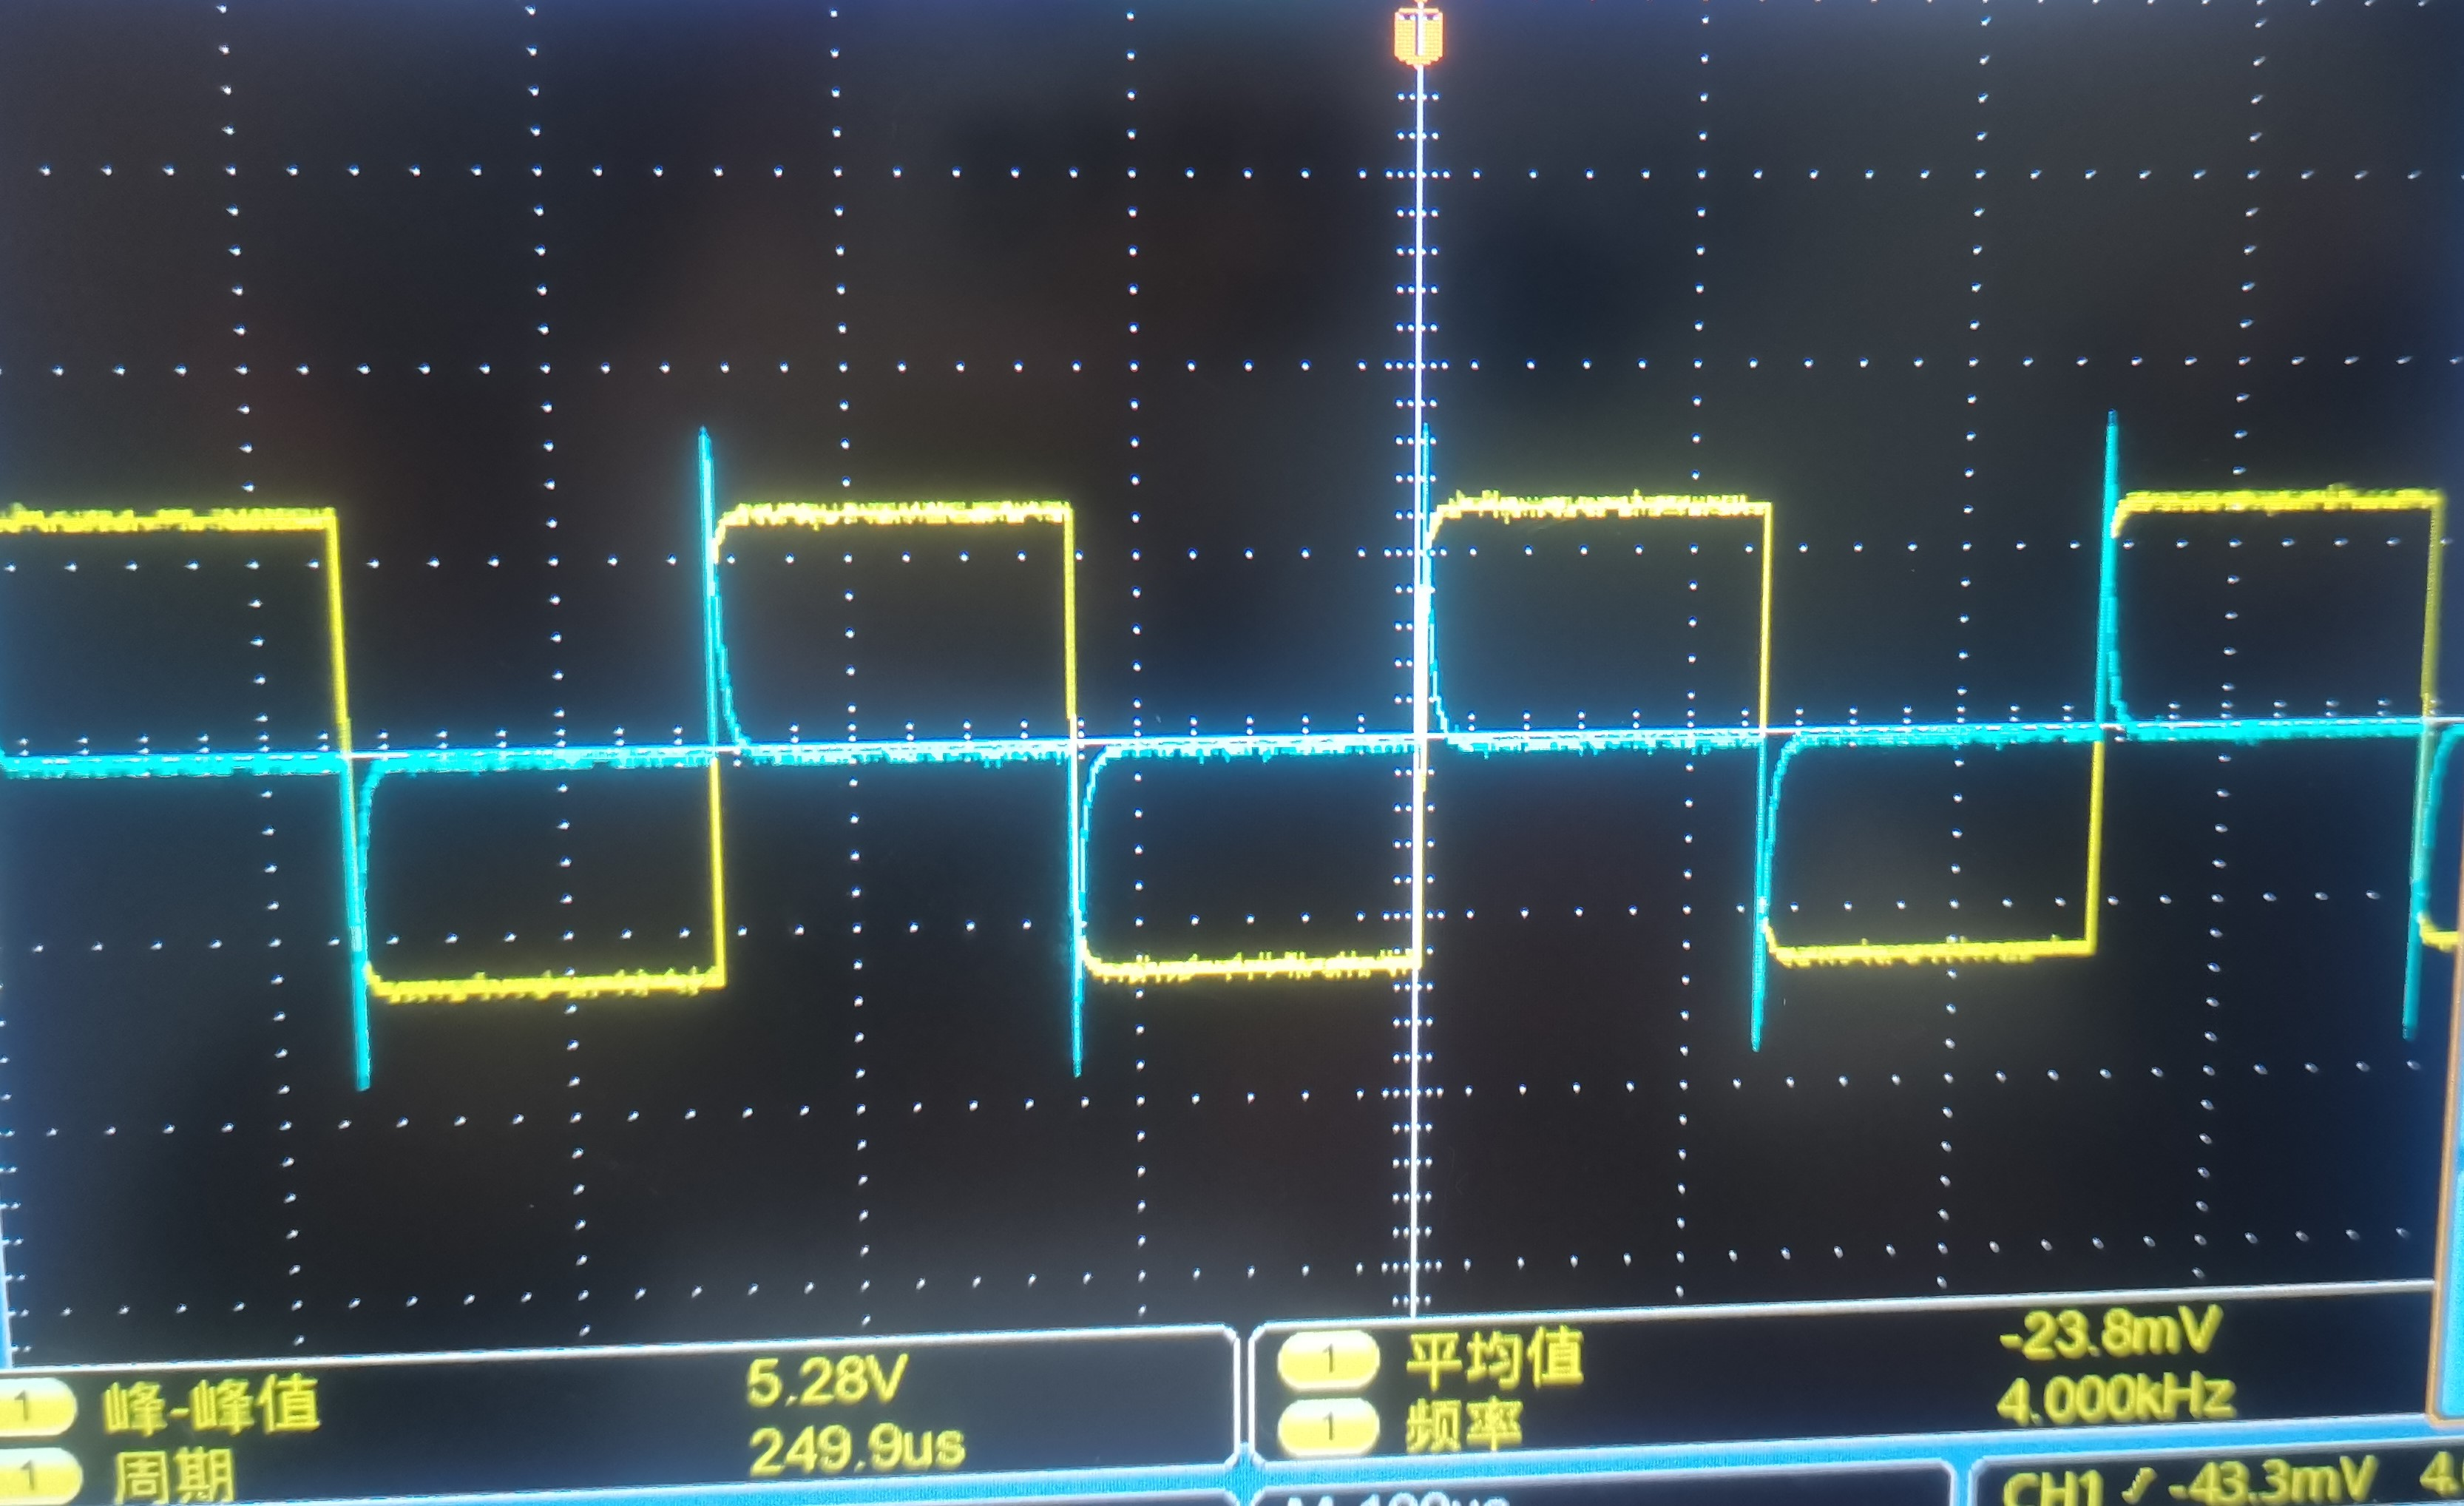
\includegraphics[width=1.9in]{尖脉冲4k.jpg}
    }
    \quad   
    \subfigure[$f=8kHz$]{
    	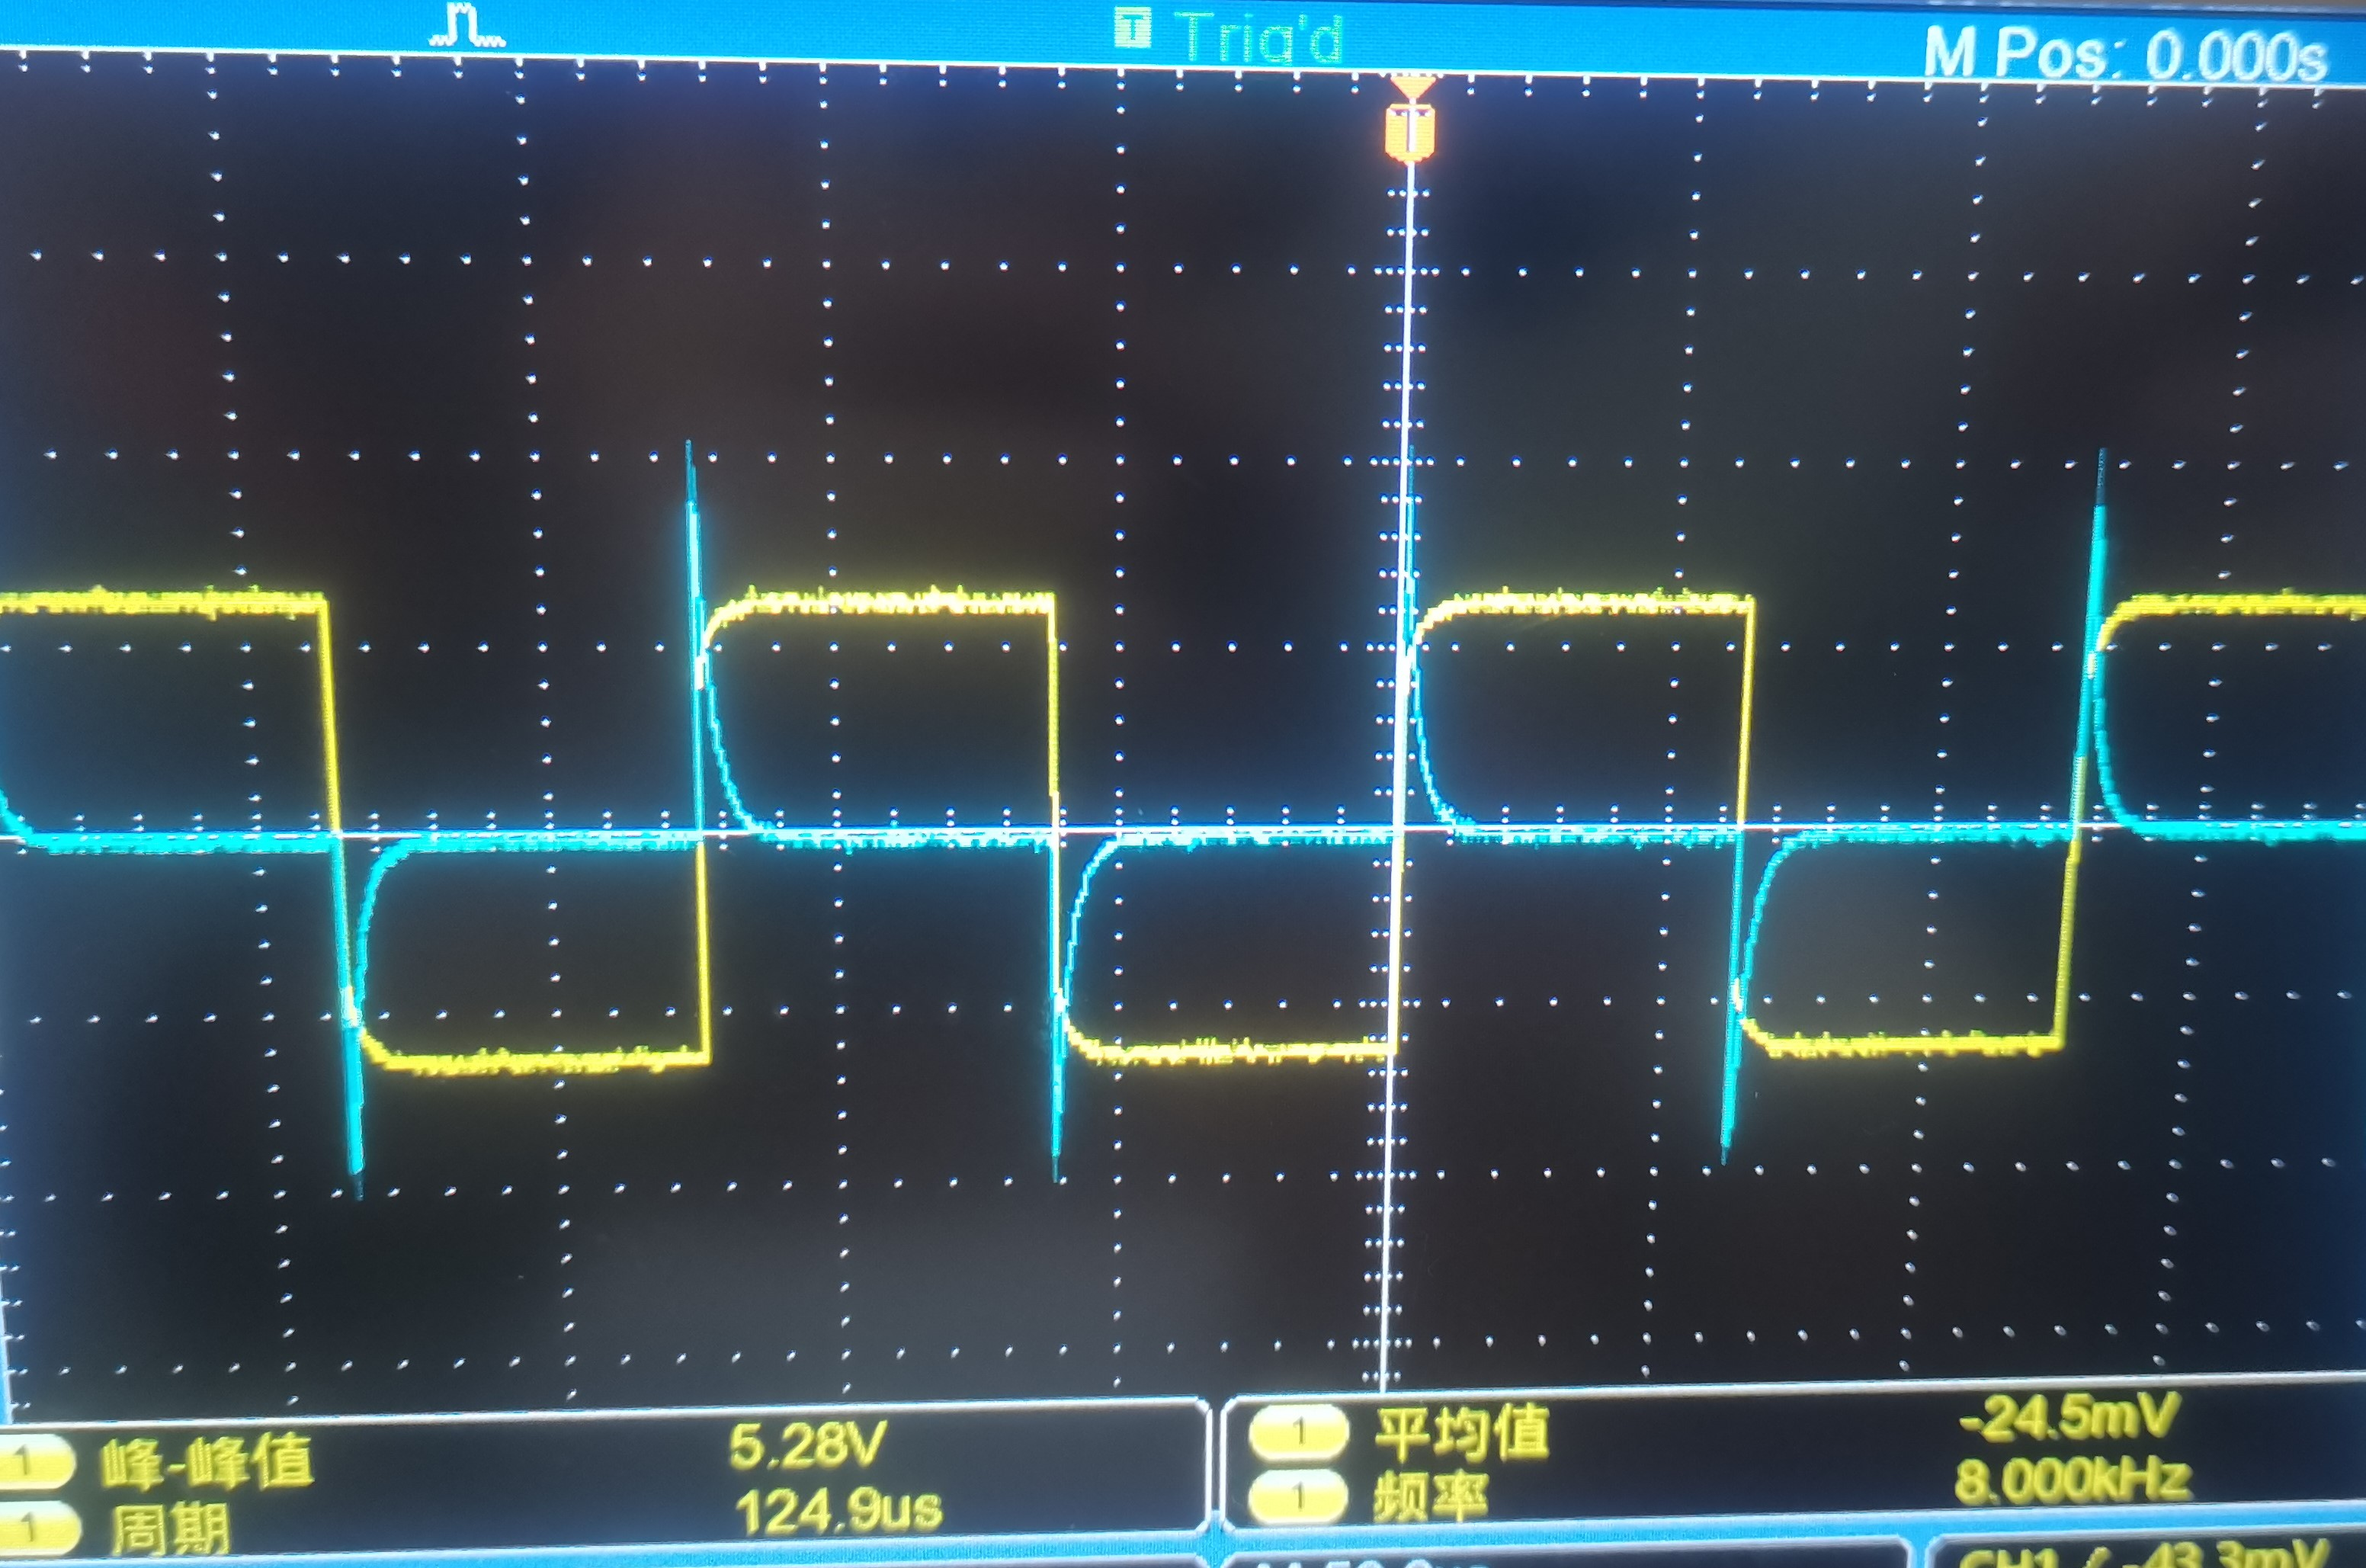
\includegraphics[width=1.9in]{尖脉冲8k.jpg}
    }
    \subfigure[$f=16kHz$]{
    	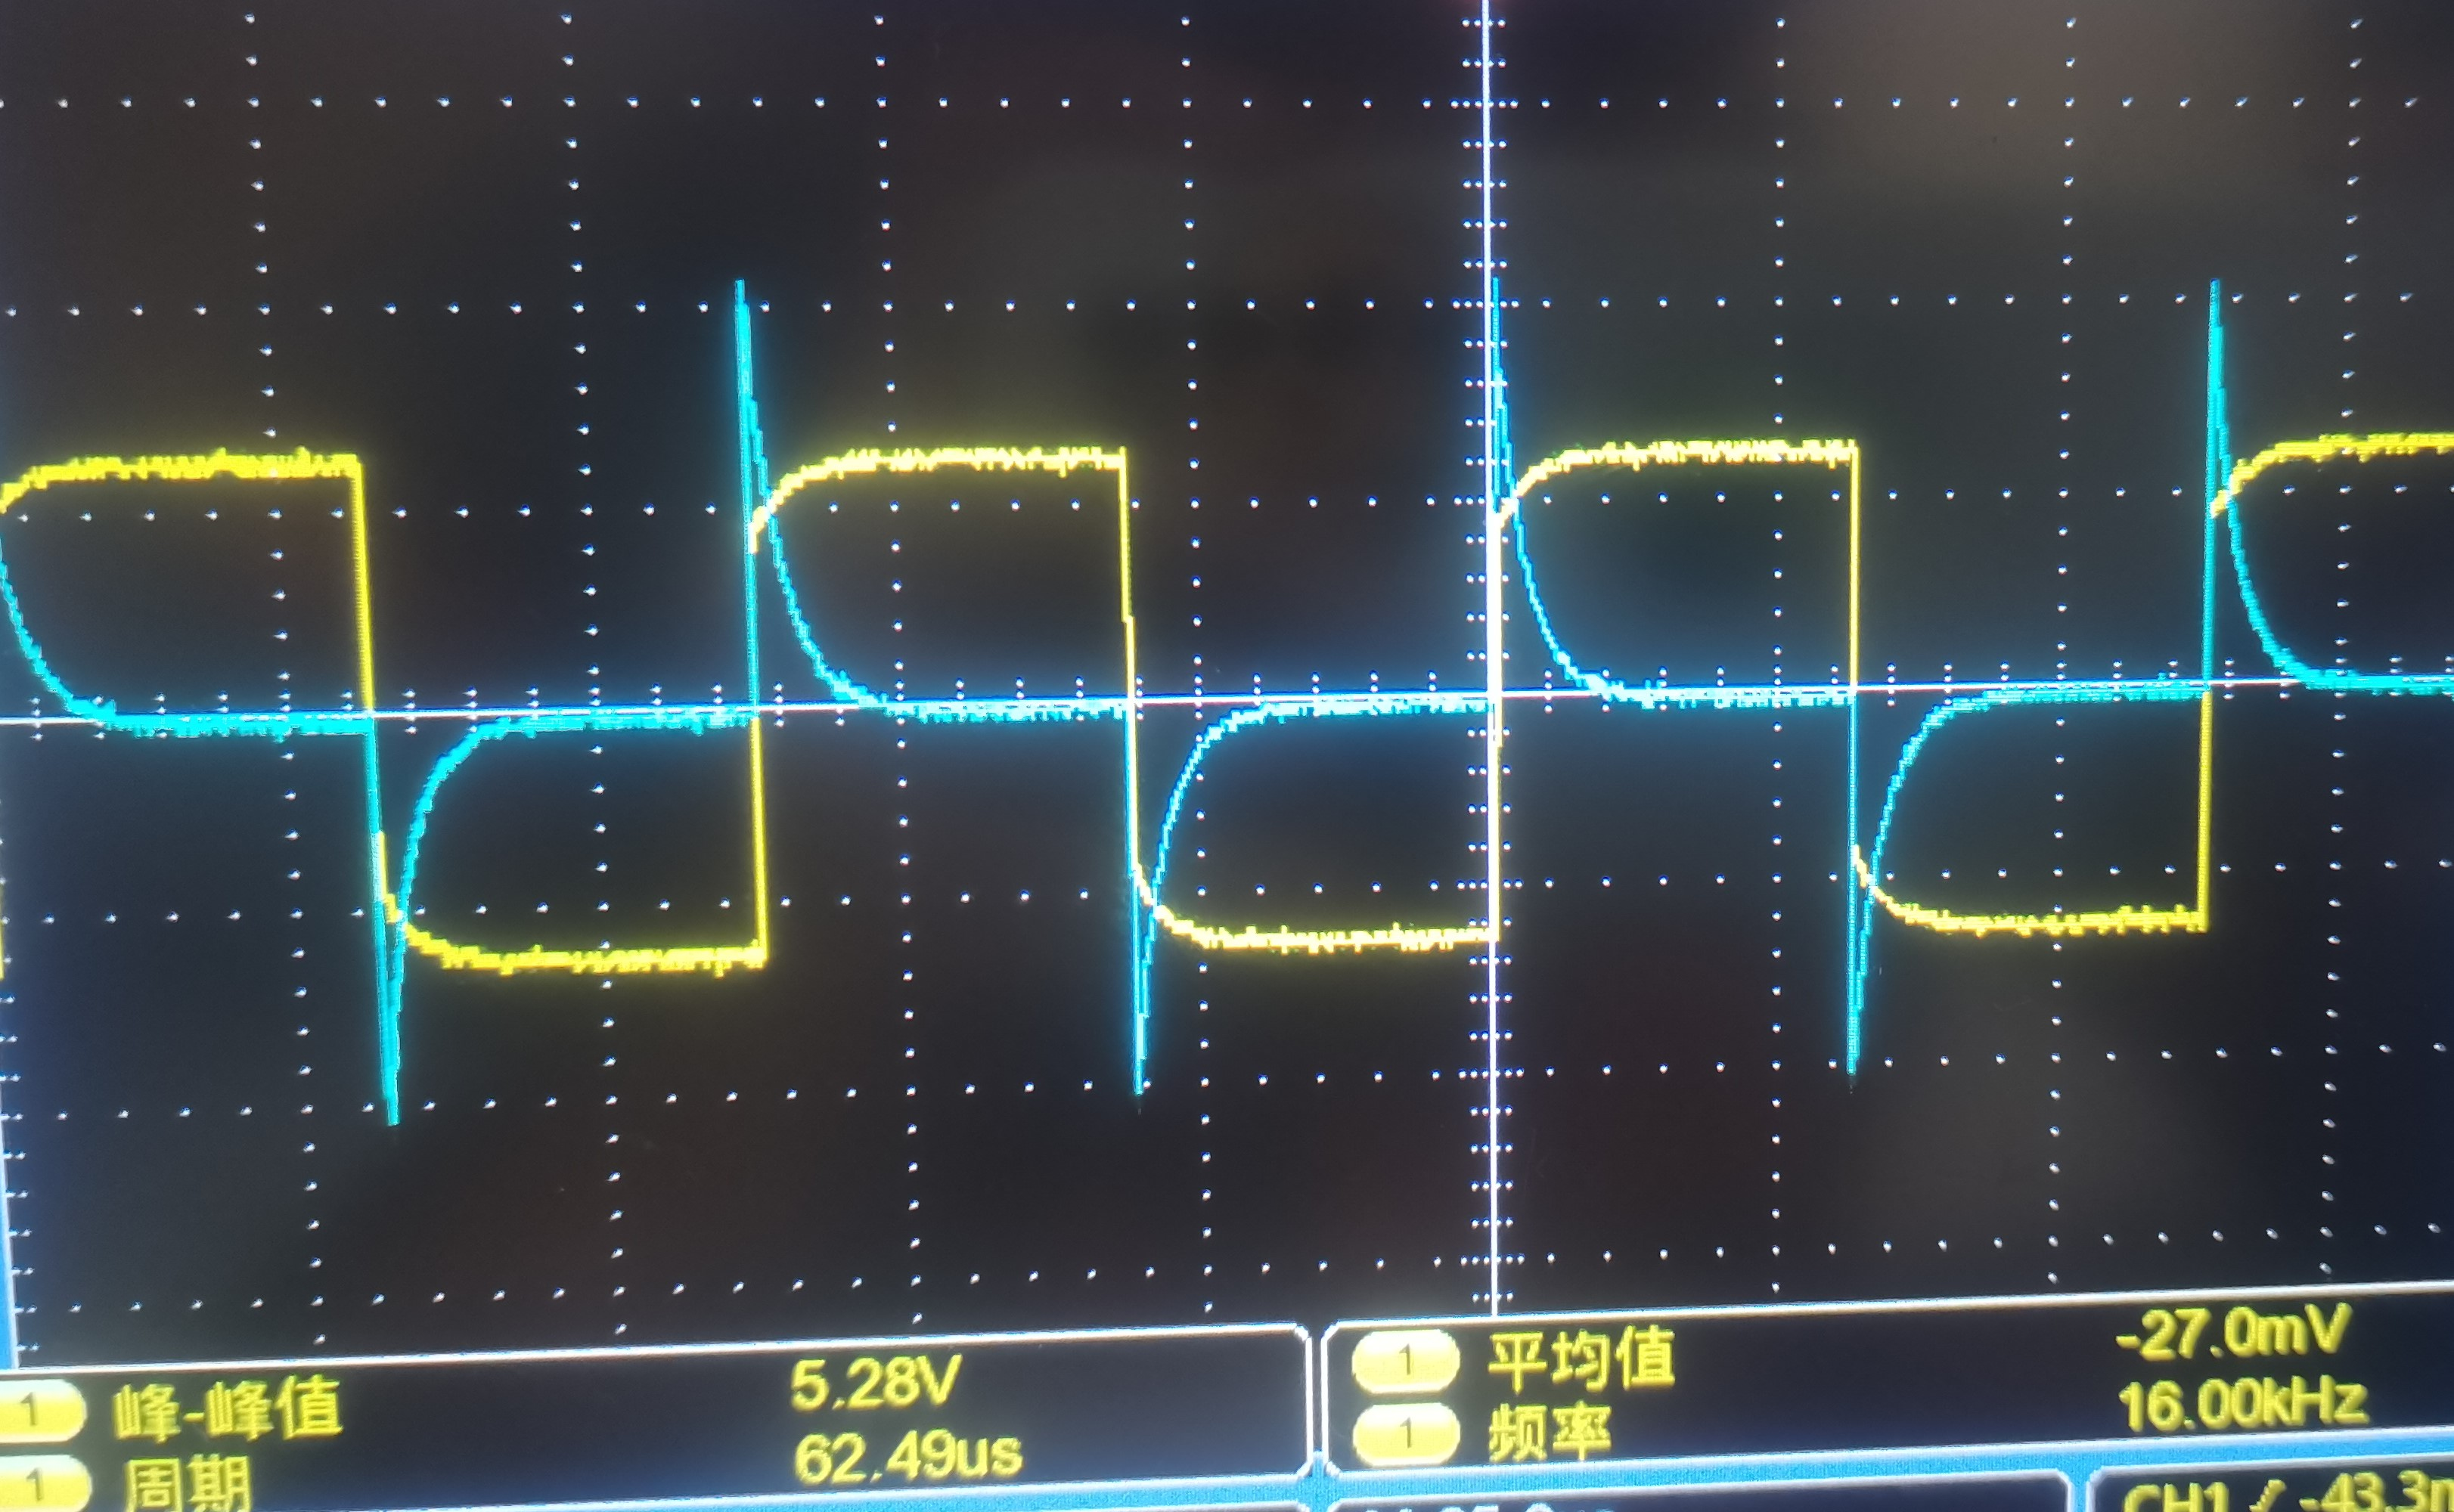
\includegraphics[width=1.9in]{尖脉冲16k.jpg}
    }
    \caption{$R=200 \Omega$ , 逐渐增大f}
    \label{fig.1}
\end{figure}

由上述波形图可以看出, 输入方波信号频率一定时, 随着电阻的增大 ,或者 当电阻一定时,随着方波频率的增大,输出尖脉冲变缓质量变差。

理论分析可知,  $u=u_{C}+u_{R}=\frac{1}{C} \int i d t+i R $,
当电阻较小的时候, 压降 $ u_{R}<<u_{C}$ , 所以有 
$u \approx \frac{1}{C} \int i d t$, 
两边对时间求导得 $i=C \frac{d u}{d t}$  。
对方波信号来说, 当信号位于高电平或者低电平的时候, 对时间的导数都是 0 , 
当方波信号发生变化的时候, 时间无限趋于 0, 所以 $ \frac{d u}{d t} \rightarrow \infty $, 
使输出信号呈现为脉冲波。同上面对积分电路的分析, 为了保证波形的完整性, 该微分电路要产生尖脉冲,
还需要使方波信号的  $\frac{T}{2} $ 远大于电路的传输延迟时间  $\tau=R C$ , 
所以增大方波频率或者增大电阻都会使输出脉冲信号质量下降。

\subsubsection{相位变化的观测(选做)}

测量条件为:$f=5kHz,C=10.435nF$

测量结果为:
\begin{center}
    \begin{tabular}{|c|c|}
        \hline  ~~~~~$R/k\Omega$~~~~~&~~~~~~$\Phi$~~~~~~\\
        \hline  0&$179^\circ$\\
        \hline $\infty$&$1.44^\circ$\\
        \hline 3.110&$90^\circ$\\     
        \hline
    \end{tabular}
\end{center}

理论计算:

当  $R=0$  时,  $\phi=180^{\circ} $

当  $R=\infty$  时,  $\phi=0 $

当$u_i$和$u_0$相位差为$90^\circ$时,
$R=X_{C}=\frac{1}{2 \pi f C}=3050\Omega$

误差分析:

$R=0 $ 时, $ \phi  $的相对误差:  $\frac{|179-180|}{180} \times 100 \%=0.56 \% $;

$R=0$  时, $ \phi $ 的绝对误差: $1.44^\circ$

当  $\phi=90^{\circ}$  时, $ R  $的相对误差: $ \frac{\mid 3110-3050\mid}{3050} \times 100 \%=1.97 \% $,

由此可以看出, 实际测量值都在合理偏差范围内。




\subsubsection{共振电路测电感、电容(选做)}

实验中,分别采用大小为 $L_1 = 10\mu H$ 与 $L_2 = 5.6mH$ 的电感、大小为 $C = 10.435nF$ 的电容进行测
量,在电路中串联一个小电阻,用小电阻两端电压的相位代替回路中电流的相位,
记录频率 $f_0$ 如下:

\begin{center}
    \begin{tabular}{|c|c|c|}
        \hline  ~~~测量频率$f_0/kHz$~~~&~~~~~实际电容$C/nF$~~~~~&~~~~~~实际电感$L$~~~~~~\\
        \hline  21.420&10.435&$5.6mH$\\
        \hline  497.60&10.435&$10\mu H$\\    
        \hline
    \end{tabular}
\end{center}

\noindent 根据共振电路的特性,有:
$$
f_{0}=\frac{1}{2 \pi \sqrt{L C}}
$$
所以实际电感为5.6mH时,电感的测量值为:
$$
L=\frac{1}{C}(\frac{1}{2\pi f_0})^2=5.29mH
$$
相对误差为:
$$
\frac{|5.6-5.29|}{5.6}\times 100\%=5.53\%
$$
实际电感为$10\mu H$时,电感的测量值为:
$$
L=\frac{1}{C}(\frac{1}{2\pi f_0})^2=9.80\mu H
$$
相对误差为:
$$
\frac{|9.80-10|}{10}\times 100\%=2.00\%
$$
相对误差较小,实际测量值都在合理偏差范围内。

\section{实验总结}

\noindent \textbf{思考题}

\noindent  \textbf{(1) 如果图形波形不稳定,总是向左或向右移动,该如何调节?}

当只有一路信号输入的时候,触发源选择被测信号所在通道;当有两路输入信号的时候,触发源选择频率较低信号所在的通道。
选好触发源后,旋转触发旋钮(Trigger)使触发电平在被测信号范围内改变,直至信号稳定。

\noindent  \textbf{(2) 获得稳定利萨如图形的必要条件是什么?}

当两个正弦信号的频率成简单的整数比,且两个正弦信号的相位差保持稳定,就能合成一个稳定、封闭的利萨如图形。

\noindent  \textbf{(3) 如果 Y 轴信号频率$ f_y $比 X 轴信号频率 $f_x $大很多,示波器上看到什么情形?相反情况呢?}

当 $f_y$ 比 $f_x$ 大很多时,示波器上显示 Y 信号图形被拉长而显示近似柱状的密集曲线;当$ f_x$ 比 $f_y$ 大很多
时,示波器上图像近似于直线。

\noindent  \textbf{(4) 若被测信号幅度太大(在不引起仪器损坏的前提下),屏幕上看到什么波形?}

只能够看到信号在屏幕范围内的波形,超出屏幕的部分无法显示,呈现为一条水平线。

\noindent  \textbf{(5) 观察利萨如图形时,如果图形不稳定,而且是一个形状不断变化的椭圆,那么图形变化的快慢与
两个信号频率之差有什么关系?}

两个信号的频率差值越大,变化越快;频率差值越小,变化越慢。

\noindent  \textbf{(6) 用逐差法处理数据的优点是什么?还有没有什么别的合适的数据处理方法,能用它通过测量得到
$\lambda$值?}

逐差法的优点在于利用所测的每一个数据,减小测量误差。

此外,利用作图法或最小二乘法拟合直线获得斜率$\lambda$,也可充分利用数据并精确处理数据。

\noindent  \textbf{(7) 式(6)中  $\Delta_{0} $ 前有一系数 $ \sqrt{2}$ , 这是为什么?}

由于实验中  $10 \lambda$  的公式为:
$10 \lambda=x_{i+10}-x_i$

其中包括两个仪器测量的量, 
故仪器导致的总误差应为  $\Delta=\sqrt{{\Delta_{0}}^2+{\Delta_{0}}^2} =\sqrt{2} \Delta_{0} $ 。

\noindent  \textbf{总结:}

在利用示波器进行波形观测时,可以利用示波器提供的自动测量模式进行测量,准确性和效率都得到了提升。

观测利萨如图形时,需要在信号发生器上对信号 1 与信号 2 进行相位对齐,否则无法得到对应相位差下的
利萨如图形。

测量声速时,需要现在40kHz附近微调频率,可以观察到,接收端幅度发生变化,
这是因为达到共振是振幅最大,选取最大振幅有利于我们的实验准确性的提高。随着
接收端与发射端距离的增大时,利萨如图形y方向幅值减小,这是由于传输距离加大后
信号的衰减增加。可以通过调节垂直定标来增大图像y方向长度以便于观察。

共振电路测电感、电容实验中,由于实验条件限制,无法直接测量电流 i 的相位。
可以在电路中串联一个大约 10Ω 的小电阻,并通过示波器测量电阻两端的电压以
实现对电流相位的测量。

共振电路测电感、电容实验中,由于输入输出的波形在很多范围内均较为相似,多次尝试后仍然
较难确定频率 $f_0$ 的值,故相对误差较大。可以先计算出理论频率值,再在其附近调节,也
许可以获得更加小的误差。

本次实验使我对利萨如图形、示波器使用、RC电路有了更深刻的认识。提高了我使用逐差法、最小二乘法处理数据的能力。
最后,感谢助教老师在本次实验中的悉心指导!


\section{附原始数据记录和预习思考题}

\begin{figure}[h]
    \centering
    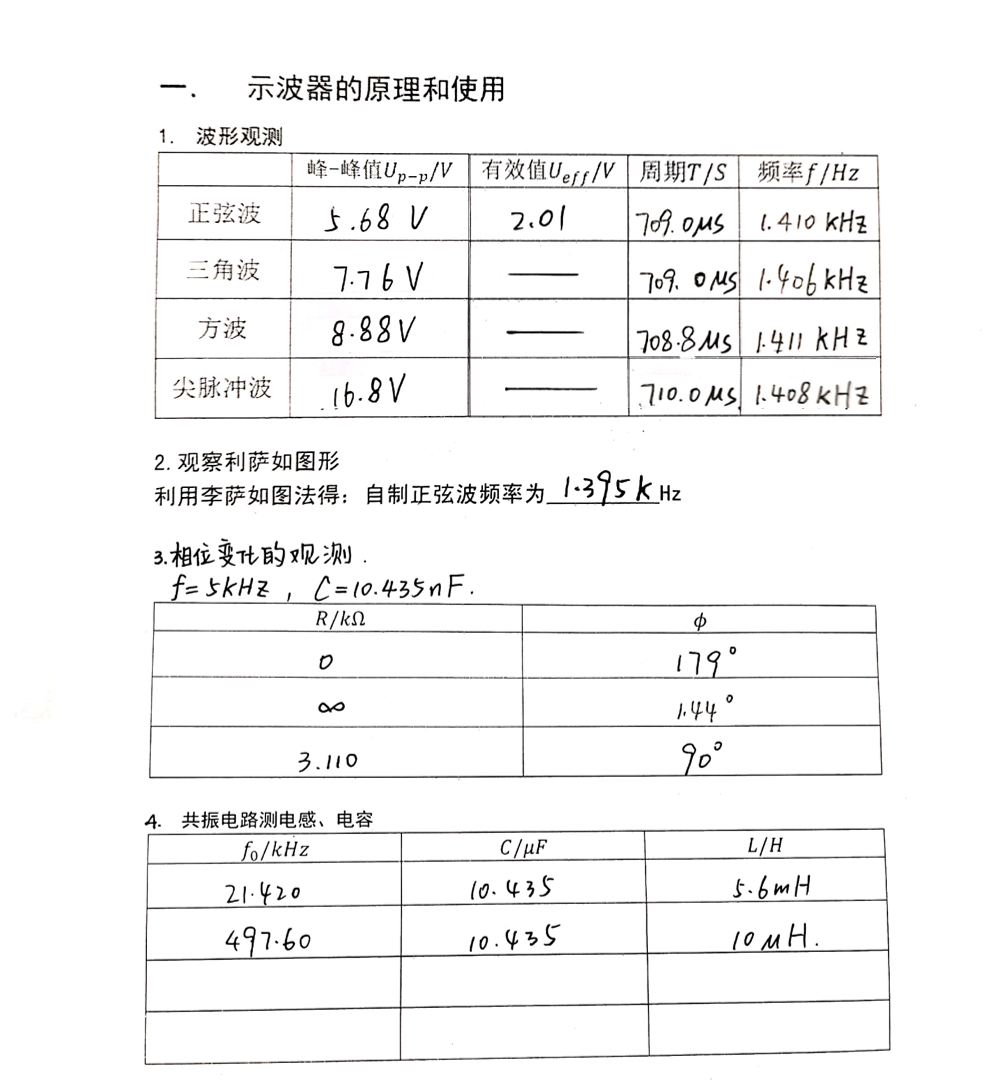
\includegraphics[scale=0.9]{记录1.png}
\end{figure}
\begin{figure}[h]
    \centering
    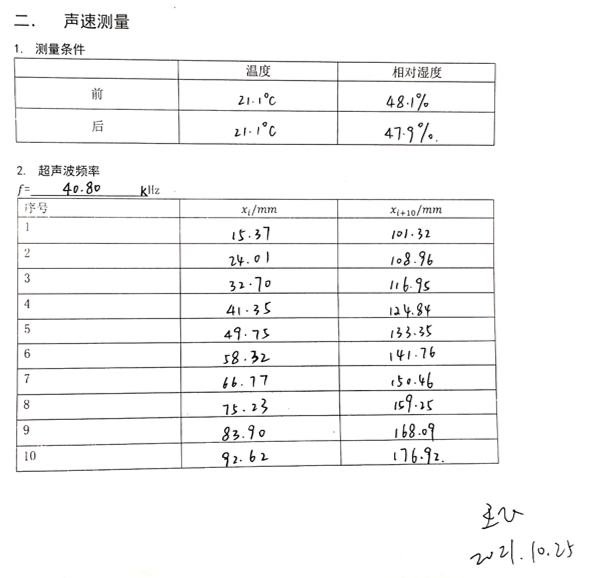
\includegraphics[scale=1]{记录2.png}
\end{figure}
\begin{figure}[h]
    \centering
    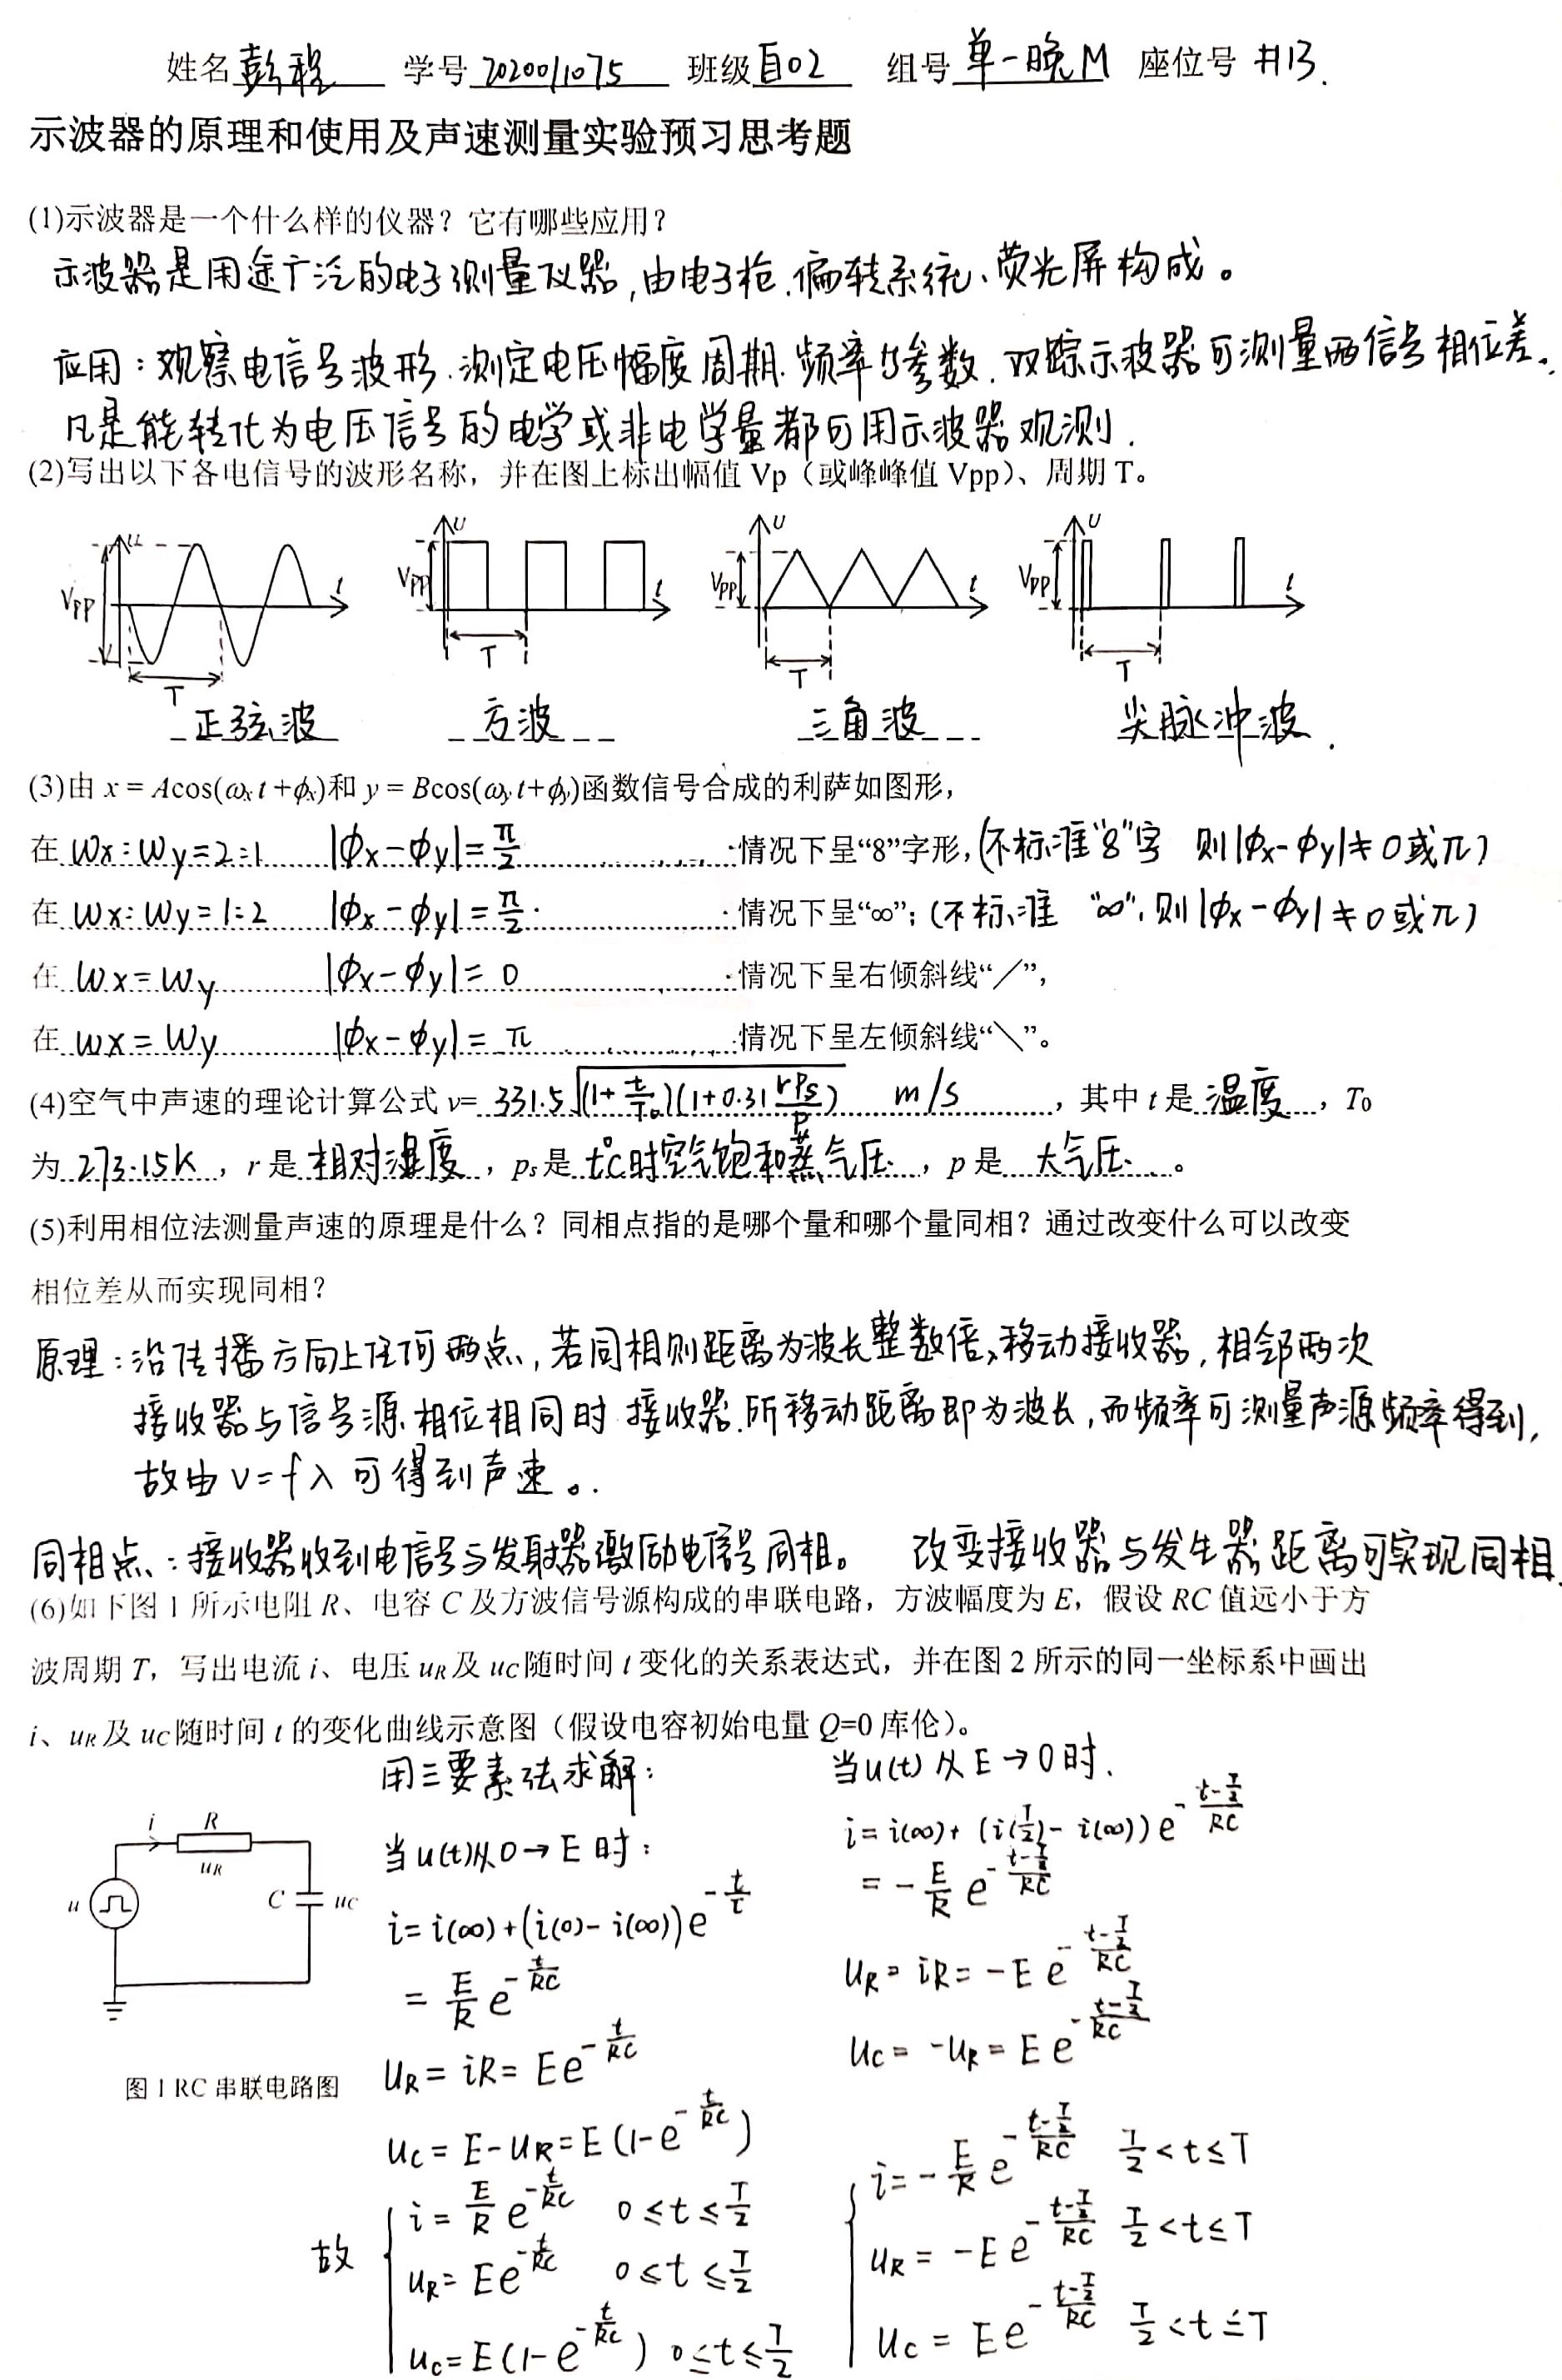
\includegraphics[scale=0.3]{预习1.jpg}
\end{figure}
\begin{figure}[t]
    \centering
    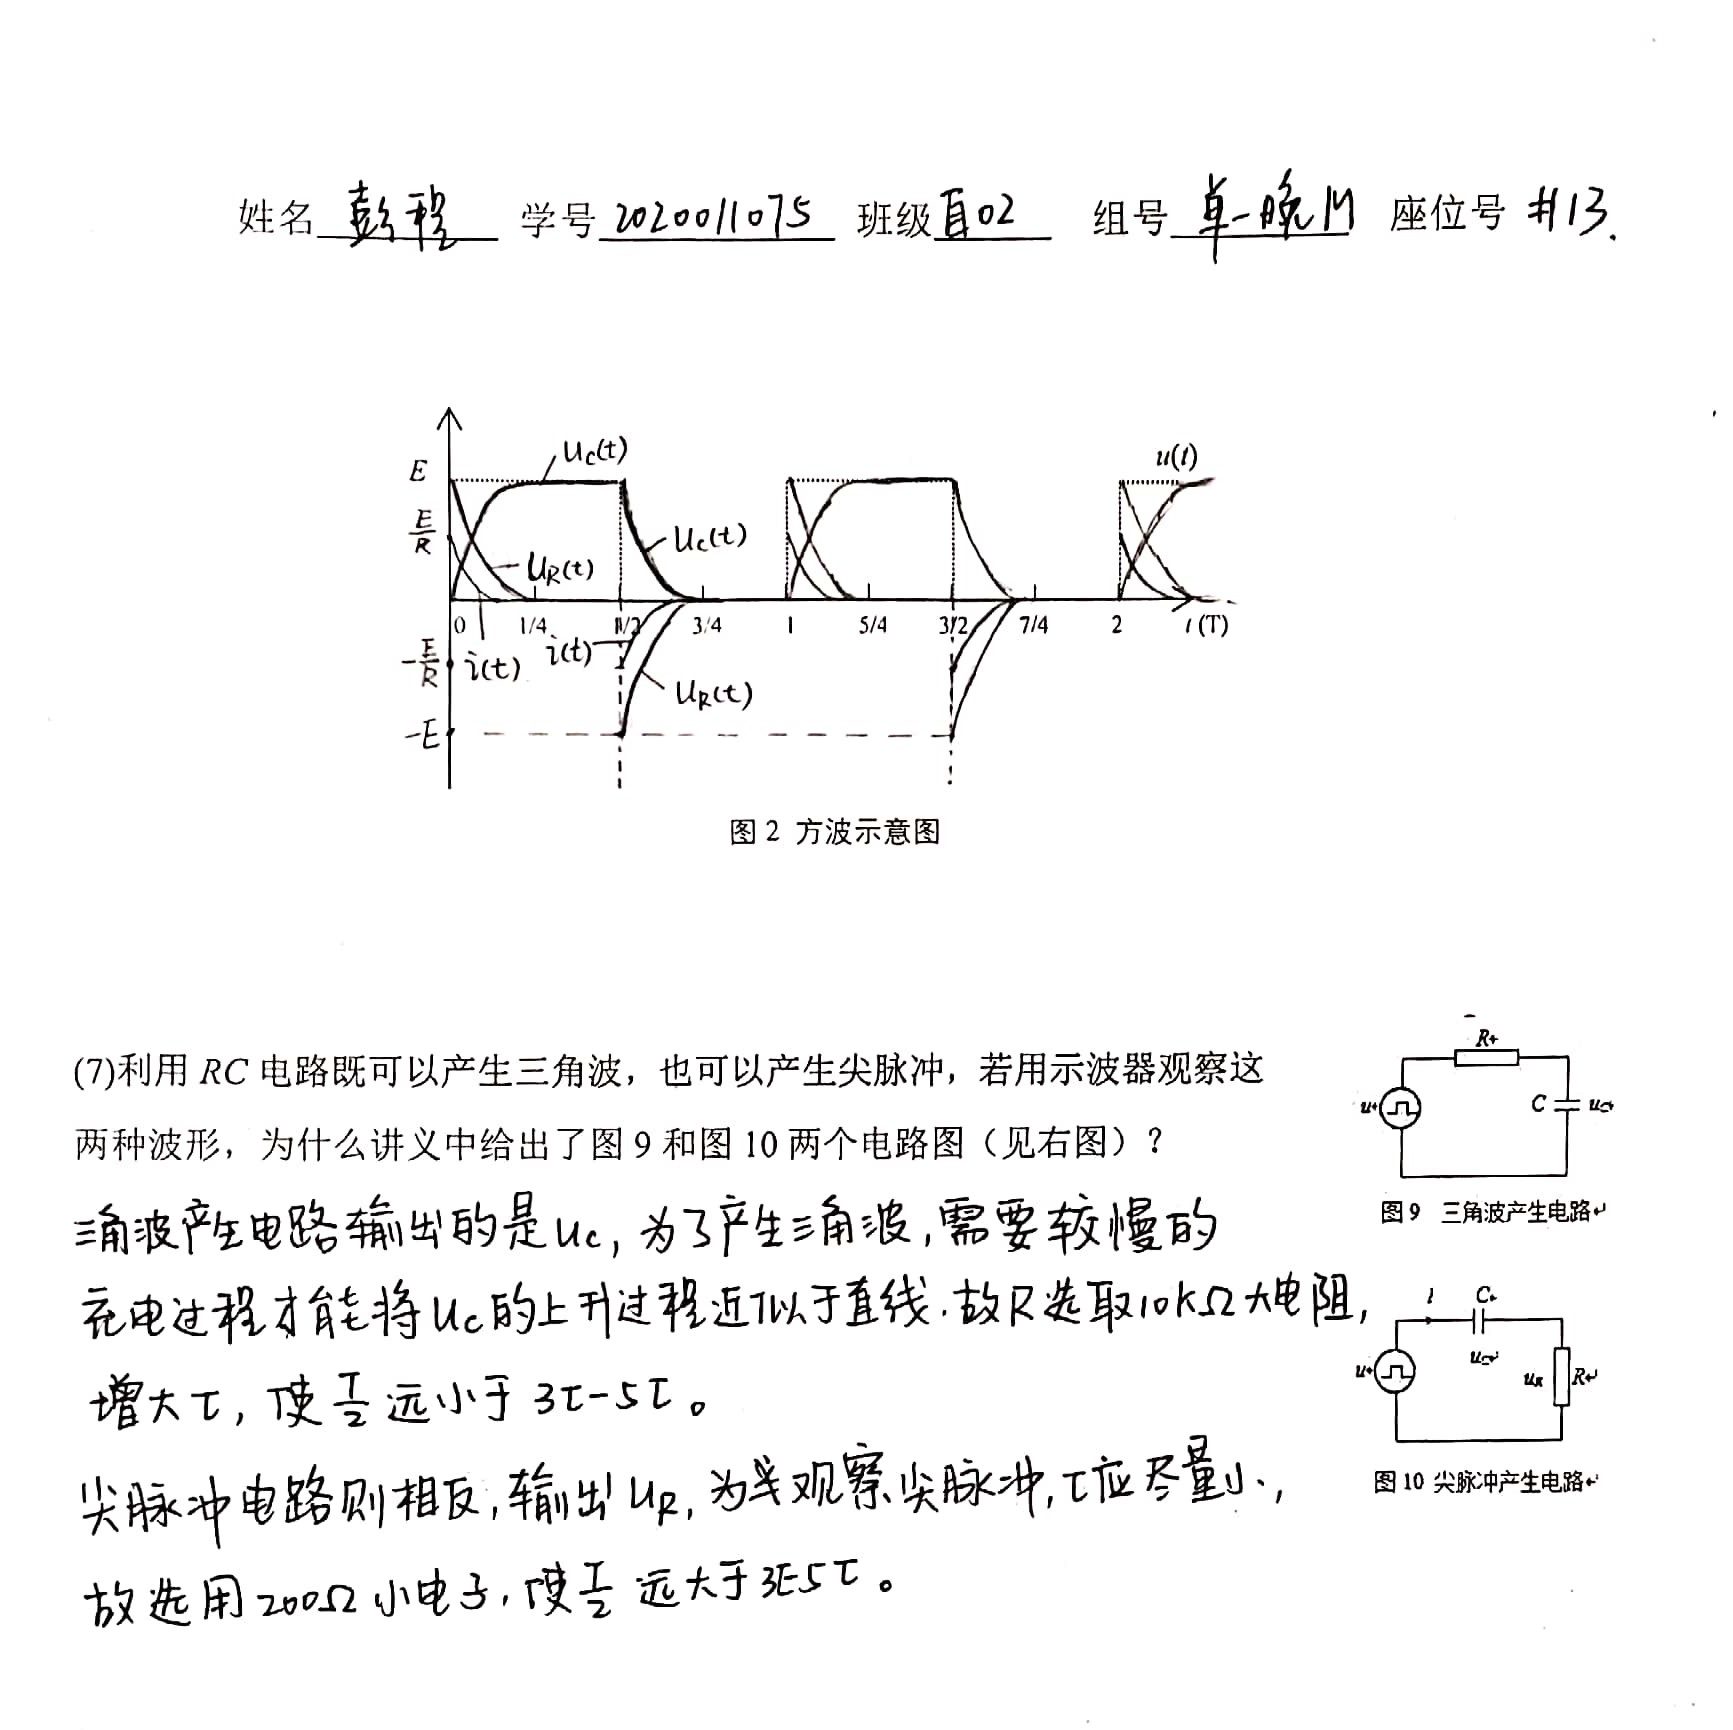
\includegraphics[scale=0.3]{预习2.jpg}
\end{figure}
\end{document}